%--------------------------------------------------------------

\chapter{Úvod}
\label{ch:uvod} % 1

%--------------------------------------------------------------

Cílem této bakalářské práce je vytvořit knihovnu pro procedurální generování struktur typu dungeon, které budou odpovídat požadavkům a parametrům vývojářů.
Knihovna by tedy měla být navržena tak, aby podchytila co možná nejvíce možných scénářů, pro které si vývojář může přát vygenerovat herní úroveň.
Funkčnost knihovny bude demonstrována na jednoduché webové aplikaci, která umožní uživatelům zadat vstupní konfiguraci a vygenerovanou strukturu poté vizualizovat.
\par
Se stále se zvyšující oblíbeností sandboxových her a s~rostoucími náklady na tvorbu herního obsahu roste také poptávka po technikách, jak tento obsah automaticky generovat.
K~tomuto účelu se využívají některé techniky procedurálního generování obsahu, díky kterým mohou vývojářská studia snížit objem práce výtvarníků a kreativních pracovníků a nabídnout hráčům variabilnější herní zážitek.
Protože tyto techniky často využívají náhodnosti nebo neurčitosti, která je činí nepředvídatelnými, může být obtížné je zakomponovat do celkové koncepce hry tak, aby vytvořený obsah přesně odpovídal požadavkům vývojářů.
Herní studia se proto snaží dosáhnout ideální rovnováhy mezi složitostí těchto algoritmů a přesností výsledků jimi navrácených.
\par
Významným herním prvkem, na kterém se tyto techniky dají uplatnit, jsou herní úrovně, ve kterých se hra odehrává.
Jejich vytváření je obvykle značně zdlouhavý a nákladný proces, který vyžaduje práci výtvarníků z~mnoha oborů a musí být realizován tak, aby výsledné úrovně odpovídaly požadovanému tempu herního postupu hráče, měly správně rozmístěné vizuální a herní prvky, byly rozmanité a případně aby se dokázaly hráčovu postupu přizpůsobovat a měnit svůj charakter.
Specifickým typem herních úrovní jsou tzv. dungeony (z~angl. podzemní žalář nebo kobka).
Dungeony se obvykle používají v~dobrodružných hrách a hrách na hrdiny (RPG~--~Role-Playing Game) a jedná se o~labyrinty, které se většinou skládají ze vzájemně propojených částí s~vysoce strukturovaným herním obsahem. Jsou tedy vhodným kandidátem pro techniky procedurálního generování.
Hráči se mohou sami rozhodnout, jakým způsobem budou dungeon prozkoumávat, jejich herní postup je však pozvolný a má gradující charakter, některé části jsou obtížnější, jiné se mohou například odemknout až po dokončení těch předchozích.
Právě tímto strukturovaným postupem se dungeony odlišují například od otevřených sandboxových světů.
Knihovna umožňující jejich automatické generování by tak mohla posloužit jako základ, na kterém by se tyto úrovně daly vytvářet efektivněji a s~menším úsilím.
\par
Text práce je rozčleněn na kapitoly.
V~první části kapitoly \ref{ch:procgen} je definováno procedurální generování obecně, druhá část obsahuje popis herní úrovně typu dungeon a v~poslední části jsou představeny techniky procedurálního generování herního obsahu, zejména herních úrovní.
Kapitola \ref{ch:soucasnost} výše představené techniky pak prezentuje v~souvislostí s~již existujícími hrami.
V~další části kapitoly jsou prozkoumány existující knihovny pro procedurální generování dungeonů.
Vlastní knihovna je navržena v~kapitole \ref{ch:navrh}.
Důraz je kladen zejména na zadávání potřebných vstupů, které umožní výslednou strukturu přizpůsobit požadavkům vývojáře.
V~další části kapitoly je navržena výstupní struktura, která bude sloužit jako prostředek pro uložení vygenerovaných dat, na jejímž základě může vývojář herní úroveň vybudovat a dále ji modifikovat.
Na závěr kapitoly je navržen způsob, jakým bude na základě těchto požadavků vytvořena výsledná struktura ve výstupním formátu s~využitím procedurálního generování.
Kapitola \ref{ch:implementace} popisuje pak samotnou implementaci knihovny.
Knihovna je realizována v~jazyce Java a nabízí uživateli objektově orientované rozhraní pro její intuitivní využití.
Kapitola \ref{ch:web} se věnuje návrhu a tvorbě webové aplikace, která knihovnu využívá a vizualizuje její výstup.
V~kapitole \ref{ch:testovani} je prověřena základní funkčnost knihovny a vlastnosti, které vykazuje.
Knihovna je zde také porovnána s již existujícími řešeními.
V~poslední kapitole \ref{ch:zaver} je práce shrnuta, jsou zhodnoceny dosažené výsledky a navrženo pokračování a rozšíření knihovny o~další funkce.

%--------------------------------------------------------------

\chapter{Procedurální generování herního obsahu}
\label{ch:procgen} % 2

%--------------------------------------------------------------

Tato kapitola pojednává o~technikách procedurálního generování.
Začátek kapitoly se věnuje procedurálnímu generování obecně a v~kontextu herních úrovní typu dungeon.
Následně je definována herní úroveň typu dungeon.
Největší část kapitoly zaujímají nejvyužívanější techniky procedurálního generování pro herní obsah, zejména pro herní úrovně, ale i jiné techniky, které mohou být v~tomto kontextu užitečné nebo zajímavé.

%--------------------------------------------------------------

\section{Definice a historie procedurálního generování}

%--------------------------------------------------------------

Tato část obsahuje úvod do procedurálního generování, je vysvětlen samotný pojem a ten je poté zasazen do kontextu generování herních úrovní typu dungeon.

%--------------------------------------------------------------

\subsection{Procedurální generování jako pojem}

%--------------------------------------------------------------

V~kontextu výpočetní techniky představuje procedurální generování tvorbu dat pomocí algoritmů (a nikoliv ručně).
Obecně se tedy jedná o~procedurální generování obsahu (zkráceně PCG -- Procedural Content Generation).
Obsah v~kontextu počítačových her pak může znamenat úrovně, textury, úkoly, nepřátelé apod.
Slovo \uv{procedurální} v~tomto případě znamená, že je obsah vytvářen pomocí počítačových procedur (nebo též funkcí, metod, rutin)\cite{lit:pcg_definition}.
Procedurální generátor může mít ve hrách mnoho podob a využití:
\begin{itemize}
    \item Metoda, která na základě vstupních parametrů (např. číslo úrovně a požadovaná velikost) vytvoří náhodné bludiště určité obtížnosti
    \item Dohledový systém, který analyzuje oblíbené a často používané zbraně hráče a vygeneruje mu vylepšené verze těchto zbraní, které bude moci během hraní získat
    \item Funkce, která generuje náhodnou hádanku typu \uv{puzzle} na určitém místě ve statickém a předem navrženém aztéckém chrámu
    \item Mechanismus, který pro rozsáhlý kontinent automaticky vygeneruje vegetaci podle podnebí
    \item Grafický systém, který náhodně generuje 3D modely obydlí domorodých kmenů
\end{itemize}
Procedurální tvorba obsahu může být pro vývojáře časově i finančně výhodná, protože stačí \textit{jednou} vytvořit generátor, který následně vyprodukuje \textit{neomezené množství} variací na herní obsah podle zadaných parametrů (viz obrázek \ref{img:pcg_workflow}).
Největší výzvou při tvorbě takového generátoru je, aby jím vytvářený obsah splňoval požadavky na kvalitu, věrnost a variabilitu.
Protože je však možnost přeměnit konečné úsilí v~potenciálně nekonečný obsah velmi lákavá, procedurální generování je předmětem neustálého zkoumání.\begin{figure}[hbt]
    \centering
    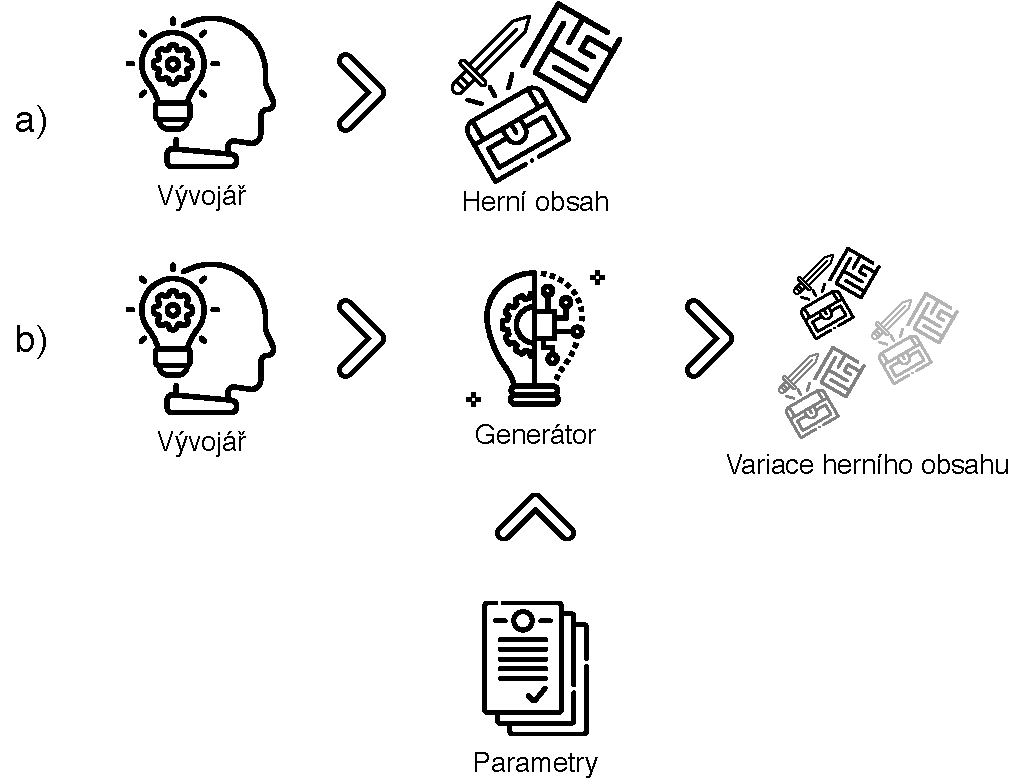
\includegraphics[width=0.8\textwidth]{obrazky/pcg_workflow.pdf}
    \caption{Porovnání způsobů tvorby herního obsahu, a) herní obsah musí tvořit vývojář ručně, b) vývojář vytvoří generátor, který generuje neomezené množství variací herního obsahu podle zadaných parametrů, pro obrázek byly použity materiály ze stránky \url{https://www.flaticon.com/}, autoři: Freepik, Kiranshastry, fps web agency, geotatah.}
    \label{img:pcg_workflow}
\end{figure}

%--------------------------------------------------------------

\subsection{Procedurální generování dungeonů}

%--------------------------------------------------------------

Velmi významnou částí procedurálního generování je generování herních úrovní typu dungeon.
Dungeony jsou prostory skládající se z~různě tvarovaných místností a chodeb, ve kterých hráč bojuje proti různým nepřátelům, řeší (nejčastěji logické) hádanky a nachází poklady.
Svým tvarem a uspořádáním často připomínají labyrint.
Herní úroveň typu dungeon je přesněji a podrobněji definována v~části \ref{sec:definice_dungeonu}.
Dungeony je možné generovat mnoha způsoby: pomocí celulárních automatů, generativních gramatik, na základě specifikovaných omezení a pravidel, pomocí genetických algoritmů atd.
Mnoho z~těchto metod vychází z~výzkumů, které se však do praxe promítají velmi zřídka.
Tyto výzkumy přesto nesou nezanedbatelný potenciál~--~umožňují generovat dungeony abstraktně jako topologickou síť bez geometrie, přizpůsobovat generátor dynamicky hráčovu postupu či chování, vytvářet úrovně \uv{na míru} pro definovanou sadu herních úkonů nebo dokonce generovat dungeony pouze zadáním požadovaných parametrů zábavy, obtížnosti a velikosti.

%--------------------------------------------------------------

\subsection{Historie dungeonů v~počítačových hrách a žánr Roguelike}
\label{ssec:historie_dungeonu_a_roguelike}

%--------------------------------------------------------------

Před definováním herní úrovně typu Dungeon je vhodné podívat se alespoň stručně na historii žánru, který stál za jejich vznikem.
Tradice her, ve kterých hráč prochází temné úrovně a bojuje v~nich proti nepřátelům sahá až do roku 1974, kdy Gary Gygax a Dave Arneson vydali velmi úspěšnou stolní hru \textit{Dungeons and Dragons}.
Tato hra obsahující prvky náhody měla velký vliv na následný vývoj počítačových her.
\par
Historicky první dochovanou hrou na hrdiny, ve které hráč procházel dungeony, bojoval s~příšerami a vylepšoval svou postavu, je hra nazvaná jednoduše \textit{The Dungeon} z~roku 1975.
Tato hra byla vytvořena pro výukový počítač PLATO provozovaný na Univerzitě Illinois v~Urbana Champaign pod názvem \textit{pedit5} a studenti si ji mohli zahrát na kterémkoliv ze 150 terminálů (i přes nevoli univerzitního systémového správce, který ji údajně často odstraňoval).
Ačkoliv byly herní úrovně v~této hře fixní, obsahovaly náhodně generované nepřátele.
\par
Velikým milníkem v~kontextu náhodně generovaných dungeonů byla hra \textit{Beneath Apple Manor}.
Tato hra z~roku 1978 byla původně vytvořena pro sériově vyráběný počítač Apple~II, takže si ji mohla zahrát širší veřejnost.
V~letech 1982 a 1983 se pak dočkala přepracování pro MS-DOS a Atari.
Cílem hráče bylo projít procedurálně generované dungeony a najít v~nich zlaté jablko.
Po cestě sbíral různé předměty a bojoval s~nepřáteli.
Grafika hry byla velmi jednoduchá především kvůli omezeným možnostem systému Apple~II.
\begin{figure}[hbt]
    \centering
    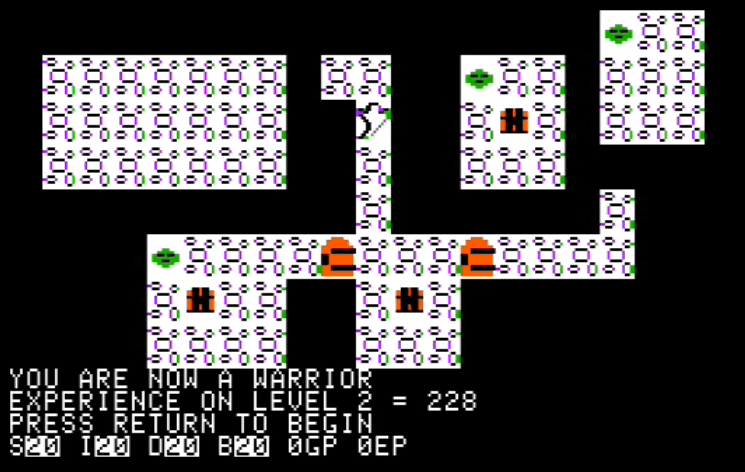
\includegraphics[width=0.6\textwidth]{obrazky/beneath_apple_manor.png}
    \caption{Ukázka ze hry \textit{Beneath Apple Manor}, která obsahovala první náhodně generované dungeony.}
    \label{img:beneath_apple_manor}
\end{figure}
\par
Koncem 70. let byla pro Unixové systémy vydána knihovna \textit{curses}, která umožňovala vývoj textových uživatelských rozhraní.
Důležitou funkcí byla možnost vkládat znaky na libovolné místo na obrazovce (podle souřadnic).
Tato knihovna byla snadno použitelná a dala vzniknout prvním počítačovým hrám s~ASCII grafikou.
V~roce 1980 vznikla hra \textit{Rogue}, která odstartovala žánr počítačových her nazvaný Roguelike (v~překladu \uv{podobné hře Rogue}).
Vznikalo mnoho her, které se více či méně podobaly původní hře \textit{Rogue}.
Spousta her přebírala pouze některé aspekty Roguelike her a proto vznikaly další dílčí žánry, které však nemají přesně vymezené hranice (např. Roguelite nebo Roguelike-like)\cite{lit:pcg_history}.
V~roce 2008 byla v~Berlíně uspořádána konference, jejímž výsledkem byl pokus o~definování žánru Roguelike.
Vznikla tzv. Berlínská interpretace\footnote{Berlínská interpretace~--~\href{http://roguebasin.roguelikedevelopment.org/index.php?title=Berlin_Interpretation}{http://roguebasin.roguelikedevelopment.org/\dots}}, která obsahuje základní charakteristiky tohoto žánru a přiřazuje jim různou důležitost.
\par \noindent
Původní koncepce žánru Roguelike z~80. a 90. let se vyznačovala těmito prvky:
\begin{itemize}
    \item Náhodně generované úrovně~--~místnosti, předměty, příšery a další prvky v~náhodně generovaných úrovních zvyšujících její opakovanou hratelnost.
    \item Tahová hra~--~každý příkaz představuje jeden pohyb nebo akci.
    Na času nezávisí, hráč si může další tah v~klidu promyslet.
    \item Jeden život~--~hráč v~Roguelike hře má pouhý jeden život.
    Musí proto postupovat opatrně.
    Pokud umře, musí začít od první úrovně, jeho herní zážitek se však bude díky procedurálnímu generování lišit.
    \item ASCII grafika~--~hry z~té doby byly reprezentovány jednoduchou ASCII grafikou, např. postavu hráče často reprezentoval znak zavináče (\texttt{'@'}).
\end{itemize}
Dnešní počítačové hry mohou být do tohoto žánru zařazeny, ačkoliv splňují pouze některá z~pravidel.
Vznikly různé variace a mutace na žánr Roguelike, jádro her však zůstává podobné~--~zkoumání (většinou) podzemních prostorů, boj proti nepřátelům, vylepšování postavy a stále jedinečný herní zážitek díky procedurálnímu generování.

%--------------------------------------------------------------

\section{Definice herní úrovně typu dungeon}
\label{sec:definice_dungeonu}

%--------------------------------------------------------------

Dungeony jsou velmi častým a populárním prvkem mnoha her na hrdiny (RPG -- Role Playing Game) a především Roguelike her.
Z~angličtiny se dungeon do češtiny překládá jako žalář, katakomba, kobka nebo hladomorna.
Jedná se tedy o~temný, uzavřený prostor složený z~místností a chodeb.
Svou strukturou a rozložením mohou dungeony připomínat labyrint.
Chodby mohou být různě široké, mohou zatáčet, vytvářet smyčky atd.
Důležité je, aby propojovaly všechny místnosti dungeonu a umožňovaly tak jeho průchodnost.
Místnosti mohou být různých tvarů i velikostí a mohou obsahovat další místnosti či chodby.
Za dungeony jsou často považovány i jeskynní komplexy, které se vyznačují méně strukturovaným tvarem a širšími chodbami, které mohou být zároveň místnostmi.
\par
\begin{figure}[ht]
    \centering
    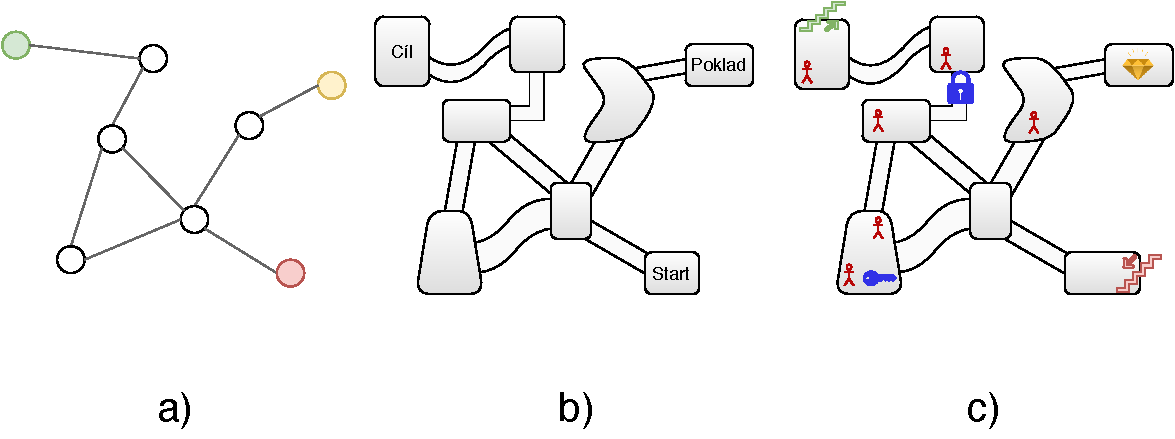
\includegraphics[width=0.8\textwidth]{obrazky/dung_topo_geom.pdf}
    \caption{Postup při konstrukci dungeonu, a) topologická struktura obsahující graf s~uzly (místnostmi), některé se speciálním významem, b) přiřazení geometrické podoby (rozměrů) chodbám a místnostem, c) rozmístění herních prvků dále upravujících postup hráče.}
    \label{img:dung_topo_geom}
\end{figure}
Dungeony v~počítačových hrách často obsahují začátek a jeden nebo více konců, které mohou vést do dalších úrovní, a v~chodbách a místnostech mohou číhat nepřátelé nebo poklady, případně různé hádanky, spínače, dveře, pasti a další prvky.
Dungeony jsou vysoce strukturované a uspořádání prvků v~nich obsažených často podléhá různým pravidlům, které souvisí především s~hratelností~--~například chodba plná nepřátel s~pokladem na konci nebo místnost s~cílem a silným protivníkem, která je v~největší vzdálenosti od začátku dungeonu.
Ačkoliv se hráč může po dungeonu volně pohybovat, jeho dosah může být omezen silnými nepřáteli nebo například zamčenými dveřmi.
Procedurální generování dungeonů tedy znamená, že je nutné vytvořit topologickou strukturu, přidělit jí geometrickou podobu a rozmístit prvky týkající se postupu (viz obrázek \ref{img:dung_topo_geom})\cite{lit:pcg_constructive_methods}.
\par
\begin{figure}[hbt]
    \centering
    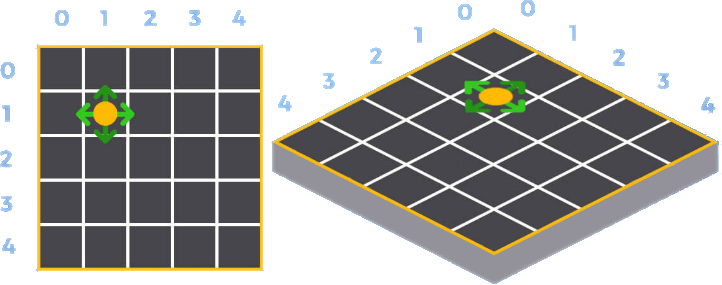
\includegraphics[width=0.9\textwidth]{obrazky/top-down_vs_isometric.png}
    \caption{Porovnání klasického zobrazení shora (vlevo) oproti isometrickému zobrazení (vpravo). Správná transformace a speciální sada grafických dlaždic tvoří iluzi třetího rozměru. Převzato z~\href{https://themindstudios.com/blog/how-to-make-game-like-brawl-stars/}{https://themindstudios.com/\dots}.}
    \label{img:top-down_vs_isometric}
\end{figure}
Dungeony mohou být dvou i trojrozměrné, mohou být předem vygenerované a omezené nebo mohou být generovány dynamicky \uv{za chodu} a mohou být tedy potenciálně nekonečné.
Dungeony mohou být vykresleny pohledem shora (z~ptačí perspektivy), ale častěji se používá některá forma axonometrie\footnote{\textbf{axonometrická projekce} je jednoduchý způsob promítání prostorových struktur do roviny}, nejčastěji isometrické zobrazení.
Pomocí správně transformovaných dlaždic a speciálně navržených grafických elementů tak mohou dungeony vypadat jako 3D, ačkoliv jsou pouze 2D (viz obrázek \ref{img:top-down_vs_isometric}).

%--------------------------------------------------------------

\section{Techniky generování herního obsahu}
\label{sec:techniky_generovani_herniho_obsahu}

%--------------------------------------------------------------

V~této části jsou probrány některé základní techniky generování herního obsahu, především dungeonů.
V~praxi se mohou využívat kombinace či modifikace různých technik.

%--------------------------------------------------------------

\subsection{Celulární automaty}

%--------------------------------------------------------------
Celulární automat je diskrétní matematický model, který znázorňuje chování nelineárního systému založeného na jednoduché sadě podmínek.
Motivací k~vytvoření prvních celulárních automatů v~polovině 20. století byla snaha John von Neumanna o~vytvoření sebe-replikujícího robota, který by dokázal sestavit druhého robota jako svou identickou kopii.
Jeho kolega, Stanislaw Ulam, navrhl využít pro tvorbu takového modelu diskrétní přístup.
Ten se mu dříve osvědčil při studiích růstu krystalů, kde jako svůj model používal diskrétní prvky v~mřížce.
Následně společně podobný systém použili k~výpočtům pohybů tekutin.
Tato metoda spočívala v~tom, že se hmota kapaliny rozdělila do diskrétních jednotek, kde se pohyb každé z~nich počítal na základě jejich sousedů.
Tím vznikl první z~celulárních automatů.
V~současnosti se celulární automaty používají v~různých oborech, především v~již zmíněné fyzice, ale také v~biologii a chemii, často v~kombinaci s~jinými systémy.
Zajímavé je, že celulární automaty v~určité přenesené formě nacházejí využití také v~informatice a umění.
Ve světě počítačů se používají jako základ pro simulace různých systému reálného světa (např. doprava), a v~některých specifických případech také při procedurálním generování.
Ve světě umění se pak používají k~tvorbě abstraktních tvarů a vzorů.
\par
Problematika celulárních automatů je dnes velice rozsáhlá a jejich typy lze dělit z~hlediska různých kritérií (dimenzí, stavů, pravidel atd).
V~této práci se spokojíme s~tím, že celulární automat lze definovat jako mřížku buněk, které jsou uspořádány v~n-rozměrném prostoru (tzv. \textit{celulární prostor}), přičemž všechny buňky mají stejný tvar (např. čtverec nebo šestiúhelník). 
Každá buňka v~určitém diskrétním, časovém bodě nabývá jednoho z~množiny možných stavů.
Velmi důležitou součástí definice celulárního automatu je počáteční stav buněk v~nulovém čase ($t = 0$).
Stav buněk v~následujícím časovém bodě ($t + 1$) (též nazývaném další \uv{generace} buněk) lze vypočítat použitím příslušného pravidla na aktuální stav každé z~nich.
Souhrnu možných pravidel se říká \textit{přechodová funkce}.
Vstupem přechodové funkce je stav vyhodnocované buňky a stavy sousedních buněk a výstupem je konkrétní výsledný stav (deterministická funkce) nebo množina možných stavů (nedeterministická funkce).
Pokud je funkce nedeterministická, obvykle bývají vrácené stavy doplněny o~rozdělení pravděpodobnosti.
U~každého celulárního automatu je nutné určit typ použitého sousedství, tedy které sousední buňky se mají brát při vyhodnocování stavu v~úvahu\cite{lit:cellular_def}.
\begin{figure}[hbt]
    \centering
    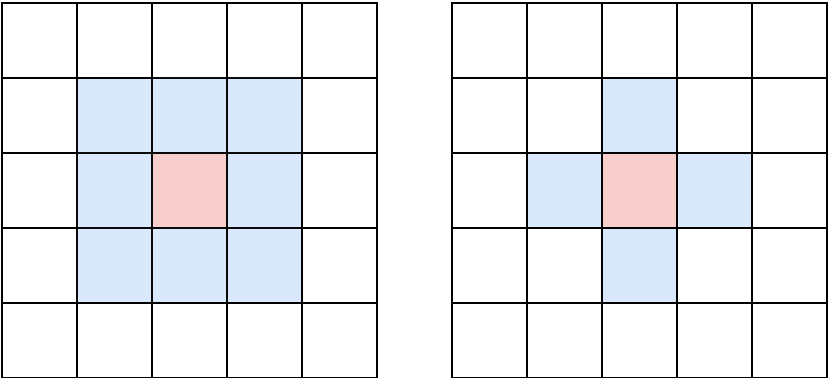
\includegraphics[width=0.5\textwidth]{obrazky/cellular_sousedstvi.pdf}
    \caption{Dvě nejčastěji používaná sousedství u~celulárních automatů~--~vlevo Moorovo a vpravo von Neumannovo. Modře znázorněné buňky se zohledňují při vyhodnocování následného stavu buňky uprostřed.}
    \label{img:cellular_sousedstvi}
\end{figure}
\par
Po několika generacích lze pozorovat, že v~závislosti na použitých pravidlech, stavech, sousedství a dalších parametrech vykazují buňky v~mřížce (systém) určité rysy chování.
Pro celulární automaty je typická jejich nelinearita a nepředvídatelnost.
Často se vyhledávají automaty, které po spuštění vykazují chování, které je užitečné pro daný specifický účel.
\par
V~kontextu procedurálního generování obsahu do počítačových her se celulární automaty používají v~některých komerčních titulech například k~simulování šíření ohně nebo proudění kapalin.
Použití celulárních automatů může být v~tomto případě výhodné, protože taková simulace je mnohem méně náročná na výpočetní čas než analytická řešení, přičemž je pro herní účely dostatečně přesná.
\par
Zajímavé řešení simulace toku kapaliny publikoval ve svém článku\cite{lit:2d_liquid_cellular} Jon Gallant, který jej využil v~systému Unity\footnote{Unity je multiplatformní systém pro vývoj 2D a 3D aplikací. \url{https://unity.com}}.
Toto řešení dělí herní plochu na čtvercovou mřížku, kde každá buňka mřížky může být v~jednom ze tří stavů~--~prázdná (nulový objem), kapalná (nenulový objem) a stěna.
Během iterace se buňky s~nenulovým objemem vyhodnocují a podle objemu a stavu sousedních buněk se objem kapaliny mezi buňkami přesouvá (v~tomto případě bylo použito von Neumannovo sousedství, které minimalizuje \uv{rozšiřování} kapalin ve spádu, např. u~vodopádů).
Toto chování je ilustrováno na obrázku \ref{img:cellular_2d_liquid}.
\begin{figure}[hbt]
    \centering
    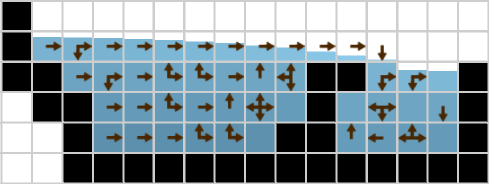
\includegraphics[width=0.8\textwidth]{obrazky/cellular_2d_liquid.png}
    \caption{Simulace kapaliny pomocí celulárního automatu. Šipky graficky znázorňují pravidlo použité pro danou buňku. Převzato z~\cite{lit:2d_liquid_cellular}.}
    \label{img:cellular_2d_liquid}
\end{figure}
Kapalina přirozeně proudí směrem dolů (simuluje vliv gravitace), případně se rozlévá do stran.
Aby vypadala simulace kapaliny přirozeně, musí simulovat také hydrostatický tlak.
Protože je účelem simulace její použití ve hrách, je důležitá především rychlost výpočtu.
Z~tohoto důvodu zavádí toto řešení zajímavý aspekt, kdy může buňka obsahovat o~trochu více kapaliny, než je běžné maximum.
Takto \uv{stlačená} kapalina poté vyhodnocuje i pravidlo, které interaguje s~buňkou o~jednu pozici výše, a snaží se kapalinu směrem vzhůru předat.
\par
Toto řešení pro simulace kapalin má výhodu v~tom, že jej lze parametrizovat podle požadovaných fyzikálních vlastností.
Vhodným nastavením počtu iterací v~herní smyčce lze dosáhnout požadovaného poměru mezi použitým výpočetním výkonem a rychlostí simulace.
Nevýhodou je nutnost procházení všech buněk mřížky a fakt, že toto řešení kapalinu rozděluje na diskrétní jednotky.
Pro dosažení vyšší přesnosti musí dojít ke zmenšení velikosti buněk, ale zároveň ke kvadratickému zvýšení jejich počtu a tím i složitosti algoritmu.
\par
Některé výzkumné práce navrhují použití celulárních automatů ke generování terénu.
Ty jsou však velice nepředvídatelné, nelze je dobře parametrizovat a proto se v~praxi nepoužívají.
\par
Dobře známy jsou celulární automaty, které vytvářejí struktury podobající se jeskynním komplexům.
V~roce 2010 proběhla v~Kalifornii konference o~procedurálním generování obsahu do počítačových her, kde byla představena metoda generování nekonečných jeskynních 2D komplexů pomocí celulárního automatu\cite{lit:cellular_cave}.
Herní prostor se v~této metodě generuje po jednotlivých mřížkách, z~nichž každá má 50x50 buněk.
Díky tomu je možné mapu generovat postupně, jak se hráč pohybuje.
Každá buňka může být v~jednom ze tří stavů: skála (neprůchozí), podlaha (průchozí) nebo stěna (na rozhraní skály a podlahy).
Na začátku algoritmu se všechny buňky nacházejí ve stavu podlahy a určité procento z~nich je náhodně změněno do stavu skály.
Při iteracích se u~každé z~buněk vyhodnocuje její okolí tak, že se sečte počet buněk v~Moorově sousedství, které jsou ve stavu skály.
Pokud součet překročí určitou hodnotu, v~další iteraci se buňka změní na skálu, v~opačném případě se změní na podlahu.
Po provedení požadovaného počtu iterací se buňky na rozhraní skály a podlahy změní na stěny.
Tato metoda je zajímavá tím, že nabízí sadu jednoduchých parametrů, pomocí kterých lze chování automatu modifikovat a získat tak jiné výsledky.
\begin{itemize}
\item \textit{r}~--~procento buněk, které jsou na začátku ve stavu skály
\item \textit{n}~--~počet prováděných iterací, více iterací má za následek širší jeskyně
\item \textit{T}~--~počet sousedních buněk, které musí být ve stavu skály, aby byla buňka vyhodnocena také jako skála
\item \textit{M}~--~maximální vzdálenost buněk Moorova sousedství (obvykle 1)
\end{itemize}
Vliv těchto parametrů na výsledné struktury však nelze jednoznačně předpovědět.
Pokud se však použití stejné parametry a stejné náhodného semínko\footnote{Náhodné semínko (random seed) je číslo, které garantuje, že s~použitím jiného semínka pseudonáhodný generátor vytvoří jinou sekvenci náhodných čísel.}, je možné vygenerovat stejně vypadající jeskyni.
Toho se využívá v~případě, kdy se hráč vrátí zpět do dřívější části jeskyně.
\par
Stejným způsobem, jakým byla vygenerována první mřížka, se vygenerují také další čtyři sousední mřížky~--~pouze se použijí jiná náhodná semínka.
Po vygenerování je potřeba zkontrolovat průchodnost jeskyní mezi první a každou ze sousedních mřížek.
Uzavřené shluky buněk ve stavu podlahy jsou propojeny tunely o~definované šířce tak, že se vyberou dvě buňky ve stavu podlahy nejblíže k~hranicím mřížky.
Na výsledných 5 mřížek se následně použije dalších \textit{n} iterací celulárního automatu, které tunely vyhladí.
\par
Autoři ve své práci zkoumali i výpočetní náročnost algoritmu.
Vytvoření jeskyně skládající se z~9 mřížek na obrázku \ref{img:cellular_cave} jim na počítači se systémem Windows 7, procesorem Intel Pentium M 1.73 GHz a 1.50 GB RAM trvalo 349 milisekund, proto algoritmus vyhodnotili jako vhodný pro generování v~reálném čase.
\begin{figure}[hbt]
    \centering
    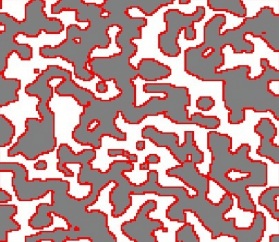
\includegraphics[width=0.5\textwidth]{obrazky/cellular_cave.png}
    \caption{Jeskyně složená z~9 mřížek o~velikosti 50x50 buněk a vygenerovaná pomocí celulárního automatu. Šedě znázorněné jsou skály, bíle podlahy a červeně stěny. Použité parametry: $r=50\,\%$, $n=4$, $T=13$, $M=2$. Převzato z~\cite{lit:cellular_cave}.}
    \label{img:cellular_cave}
\end{figure}
\par
Celulární automaty mají potenciál pro využití v~počítačových hrách.
Reálně se používají pro jednoduché simulace fyzikálních jevů a ačkoliv nejsou kvůli nedostatečným možnostem jejich ovládání příliš vhodné pro procedurální generování, lze je použít v~kombinaci s~dalšími metodami.

%--------------------------------------------------------------

\subsection{Generativní gramatiky}

%--------------------------------------------------------------

Generativní gramatika je formální systém generující určitou množinu řetězců nad určitou abecedou.
Pojem generativní gramatika v~50. letech 20. století poprvé definoval \uv{otec moderní lingvistiky}, Američan Noam Chomsky, a sice jako gramatiku s~pravidly, která umožňují vytvářet kombinace slov, ze kterých vznikají gramaticky správné věty v~daném jazyce.
Formálně je generativní gramatika čtveřice $G=(V, V_{T}, P, S)$, kde $V$ je konečná množina neterminálních symbolů, $V_{T}$ je konečná množina terminálních symbolů, $S$ je tzv. výchozí symbol (platí, že $S \in V-V_{T}$) a $P$ je konečná množina dvojic (nazývaných přepisovací pravidla) tvaru $(u, v)$ kde $u \in (V-V_{T})^*, v \in V^*$, přičemž $u$ je neprázdný řetězec.
Tato pravidla se zapisují v~podobě $u \rightarrow v$ a čtou jako \uv{přepiš $u$ na $v$}.
Postupnou aplikací přepisovacích pravidel na počáteční symbol $S$ a z~něj vzniklé řetězce se vytvářejí derivace (též posloupnosti řetězců nebo slovní formy), až dokud v~řetězci nezůstanou pouze terminální symboly.
Jazyk definovaný gramatikou $G=(V, V_{T}, P, S)$ je pak množina $L(G) = \{w: w \in V^*_T, S \Rightarrow^*w\}$\cite{lit:mat_popis_jazyku}.
Na základě generativních gramatik vznikly další druhy gramatik, například gramatiky grafů nebo tvarů, které se liší svou lingvistickou definicí, kdy např. jako terminální symboly používají uzly nebo tvary.
\par
\begin{figure}[hbt]
    \centering
    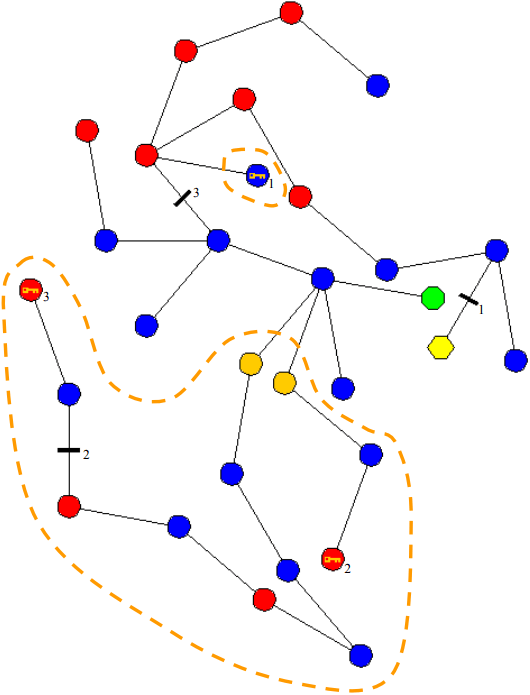
\includegraphics[width=0.4\textwidth]{obrazky/graph_adams.png}
    \caption{Graf herní úrovně vygenerovaný pomocí generativní gramatiky a parametrů pro velikost, obtížnost a zábavu. Převzato z~\cite{lit:graph_adams}.}
    \label{img:graph_adams}
\end{figure}
David Adams ve své práci\cite{lit:graph_adams} představil systém, který generuje topologické celky ve formě grafů na základě číselných parametrů definujících hratelnost.
Výsledné grafy jsou tvořeny uzly představujícími místnosti a hranami, které reprezentují propojující chodby (viz obrázek \ref{img:graph_adams}).
Grafy jsou doplněny tzv. aktivátory (oblasti, kterými musí hráč projít, např. přepínač nebo klíč), dveřmi, které se pomocí aktivátorů otevírají, nepřáteli a odměnami.
Generování grafu probíhá tak, že hledací algoritmus analyzuje výsledky přepisovacích pravidel a vybírá v~danou chvíli to nejvhodnější.
Toto chování (tzv. strategie) je pevně zakódované a neměnné.
Pro tvorbu jiných typů úrovní by bylo nutné vytvořit novou sadu pravidel.
Systém přijímá tři parametry, které souvisí s~hratelností:
\begin{itemize}
\item velikost~--~průměrná vzdálenost od začátku do konce a počet objektů v~grafu
\item obtížnost~--~počet a koncentrace nepřátel, počet aktivátorů a dveří, rozsáhlost a rozvětvenost grafu
\item zábava~--~variabilita úrovní, poměr velikosti úrovní a počtu objektů
\end{itemize}
Práce však nenabízí žádné řešení pro převod grafu do geometrické podoby.
Autor v~závěru přiznává, že převod grafu do podoby fyzické herní úrovně by byl velmi obtížný.
\par
Zajímavý princip generování dungeonů na základě úkolů ve hře představil ve své práci Joris Dormans\cite{lit:graph_dormans}.
V~této práci jsou použity grafové gramatiky, kde postupnou aplikací přepisovacích pravidel vzniká orientovaný graf mise, což je posloupnost úkolů, které musí hráč vykonat.
Vygenerovaná kostra grafu je poté asociována s~pravidly tvarové gramatiky.
Rekurzivní aplikací těchto pravidel a úpravou velikostí tvarů pak vzniká herní úroveň, která je vhodná pro vygenerovaný graf mise.
Výhodou je, že grafovou a tvarovou gramatiku lze používat nezávisle na sobě, to znamená, že pro graf mise lze vytvořit neomezené množství geometrických úrovní, a vygenerovanou geometrickou úroveň lze použít pro různé mise.
Nevýhodou je, že vytvořené gramatiky jsou velmi specifické, jejich tvorba je složitá a neflexibilní.
Autor do své práce nezahrnul žádné parametry, veškeré chování definoval přepisovacími pravidly.
\par
Odpovědí na tento problém může být práce\cite{lit:graph_der_linden} představená v~roce 2013 na konferenci Artificial Intelligence and Interactive Digital Entertainment.
V~ní vývojář na začátku určuje tzv. herní slovník akcí, který se skládá z~dvojic \textbf{sloveso~--~obsah}, například \textbf{získat} (sloveso) \textbf{klíč} (obsah).
Tyto akce jsou složené a skládají se z~posloupnosti podakcí.
Jednotlivé posloupnosti jsou v~disjunktním vztahu~--~splněním kterékoliv posloupnosti se splní i akce samotná.
Posloupnosti tedy představují předpisy, jakými lze akce splnit.
Například akci získání klíče lze provést takto: otevřít truhlici $\rightarrow$ sebrat klíč \textit{NEBO} porazit nepřítele $\rightarrow$ prohledat jeho tělo.
Na základě vývojářem definovaného herního slovníku pak popisovaný algoritmus vytváří grafové gramatiky, které generují grafy akcí hráče podobné grafům v~práci Jorise Dormanse \cite{lit:graph_dormans}.
Generování herního prostoru na základě vygenerovaných grafů je pak na vývojáři samotném.
Autoři demonstrovali způsob, jak takový generátor vytvořit, na skutečné hře (Dwarf Quest), viz. obrázek \ref{img:graph_der_linden}.
\begin{figure}[hbt]
    \centering
    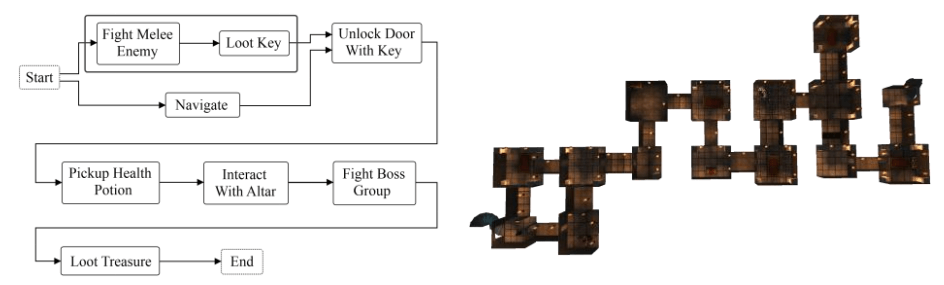
\includegraphics[width=0.75\textwidth]{obrazky/graph_der_linden.png}
    \caption{Ukázka vygenerované herní úrovně (vpravo)
    na základě grafu herních úkonů (vlevo). Převzato z~\cite{lit:graph_der_linden}.}
    \label{img:graph_der_linden}
\end{figure}
\par
Moderní výzkum generativních gramatik v~kontextu procedurálního generování se převážně týká generování struktur herních úrovní odpovídajících požadovaným parametrům hratelnosti.
Tento přístup je jedinečný v~tom, že vývojář nemusí řešit \textit{způsob}, jakým bude herní úroveň vygenerována.
Stačí mu charakterizovat herní prvky, jako jednotlivé lokace nebo akce, a generátor vytvoří odpovídající graf herní úrovně.
Nevýhodou je složitá tvorba takových generátorů.
Jakákoliv změna v~herních prvcích může přepisovací pravidla dramaticky ovlivnit.
Výzkumné práce zabývající se použitím generativních gramatik ke generování herních úrovní navíc jejich fungování často demonstrují na velmi jednoduchých příkladech.
Jimi uváděné parametry nebo pravidla jsou pro použití ve skutečných počítačových hrách často nedostačující.
Jejich potenciál pro komerční využití je tudíž předmětem dalšího zkoumání.
Použití grafových struktur jako obecné reprezentace místností se však ukazuje jako velmi užitečné a ve skutečnosti se také široce využívá.
Vývojáři ale stále musí řešit problém, jak podle této abstraktní grafové reprezentace vytvořit geometrickou podobu herních úrovní.

%--------------------------------------------------------------

\subsection{Prohledávací metody}

%--------------------------------------------------------------

Prohledávací metody se pomocí evolučního nebo jiného stochastického vyhledávacího či optimalizačního algoritmu snaží najít řešení s~požadovanými vlastnostmi.
Předpokladem pro jejich využití je, že ve stavovém prostoru takové řešení skutečně existuje.
Algoritmus iterativně prohledává stavový prostor tak, že postupně upravuje aktuální řešení.
Pokud se nové řešení vlastnostmi přibližuje hledanému řešení, je zachováno, v~opačném případě je zahozeno.
Prohledávací metoda se neobejde bez základních komponent:
\begin{itemize}
    \item Vyhledávací/optimalizační algoritmus -- jádro prohledávací metody. Představuje způsob, jakým se metoda postupně přibližuje k~výsledku.
    \item Reprezentace obsahu -- jakým způsobem lze jednotlivá řešení popsat. To zahrnuje množinu všech vlastností, které jsou pro algoritmus důležité a \uv{uchopitelné}. Může se jednat například o~pole hodnot nebo graf.
    \item Jedna nebo více vyhodnocovacích funkcí -- tato funkce dokáže převést určitou vlastnost obsahu na číselnou podobu, aby bylo možné jednoznačně určit, která je při posuzování výsledků lepší nebo horší.
\end{itemize}
Jedním z~dobře známých vyhledávacích algoritmů je stochastický \textbf{evoluční algoritmus}.
Tento algoritmus je inspirován principem Charlese Darwina o~přirozeném výběru.
V~tomto algoritmu jsou vlastnosti a chování jedinců popsány pomocí \textit{chromozomů}, což jsou nejčastěji řetězce nul a jedniček popisujících pozici jedince v~prostoru možných řešení.
Chromozom je složen z~\textit{genů}, což jsou nejmenší, dále nedělitelné jednotky.
\textit{Populace} je určitá konečná množina jedinců v~dané generaci.
\textit{Fitness hodnota} představuje číselné hodnocení kvality jedince a je výstupem vyhodnocovací funkce.
V~každé generaci dojde k~\textit{selekci} jednotlivců (též nazývaných kandidáti) a zůstanou zachováni ti, kteří mají nejlepší hodnocení.
Nejlépe hodnocení jedinci se mohou reprodukovat, nejhůře hodnocení jedinci jsou z~populace vyřazeni.
Pro selekci se běžně používá metoda, která lépe hodnoceným jedincům přiřadí větší pravděpodobnost, že budou vybráni k~reprodukci pro další generaci.
Samotná reprodukce, nebo též \textit{křížení}, pak představuje výměnu částí chromozomů mezi dvěma vybranými jedinci (rodiči).
Potomky se pak mohou stát oba dva nebo jeden z~nich.
Poslední fází je \textit{mutace}.
U~potomků se projde celý chromozom a s~velmi malou pravděpodobností dojde ke změně genu.
K~tomu dochází proto, aby byly do nové generace zaneseny vlastnosti, kterými nemuseli disponovat žádní jedinci z~předchozí generace\cite{lit:pcg_search_based_methods}.
\par
Zmíněný evoluční algoritmus dokáže vyhledávat ideální řešení bez nutnosti prohledávat celý stavový prostor.
Nejčastějším problémem je však výběr vhodné reprezentace chromozomů a nalezení vyhodnocovací funkce, která dokáže správně zachytit požadované vlastnosti.
Jednotlivé kvalitativní vlastnosti je však často obtížné reprezentovat jednoduchými číselnými hodnotami, proto se v~praxi používají pokročilé algoritmy, které dokážou využít více vyhodnocovacích funkcí současně (například elitistický nedominovaný třídící genetický algoritmus NSGA-II).
\par
Daleko jednodušší metodou lokálního prohledávání je metoda Hill-climbing (metoda lezení do kopce).
Tato metoda využívá taktéž funkci pro ohodnocení kvality a jako další řešení vybírá nejlépe ohodnocenou možnost.
Pokud je však ohodnocení kvality následného řešení horší než u~aktuálního řešení, algoritmus končí a výsledkem je aktuální řešení (viz obrázek \ref{img:hill_climbing1}).
\begin{figure}[hbt]
    \centering
    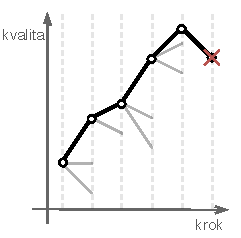
\includegraphics[width=0.4\textwidth]{obrazky/hill_climbing1.pdf}
    \caption{Znázornění algoritmu Hill-climbing. V~jednotlivých krocích může být více možných následných řešení s~různým ohodnocením kvality. Vybráno je vždy to nejkvalitnější. Pokud nelze v~dalším kroku dosáhnout kvalitnějšího řešení, než je řešení aktuální, algoritmus končí.}
    \label{img:hill_climbing1}
\end{figure}
\par
Další využívanou stochastickou metodou lokálního prohledávání je \textbf{simulované žíhání}.
Tato metoda vznikla za účelem, aby vyřešila problémy s~lokálními extrémy, které vedly k~častým neúspěchům metody Hill Climbing (viz obrázek \ref{img:hill_climbing2}).
\begin{figure}[hbt]
    \centering
    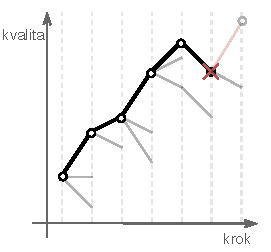
\includegraphics[width=0.4\textwidth]{obrazky/hill_climbing2.pdf}
    \caption{Znázornění algoritmu Hill-climbing, který byl ukončen předčasně z~důvodu lokálního extrému, a tudíž se mu nepodařilo nalézt řešení s~nejlepším ohodnocením.}
    \label{img:hill_climbing2}
\end{figure}
Jak již název napovídá, metoda vychází z~metody tepelného opracování kovů, kdy se kovy nejdříve zahřejí (čímž se atomy uvolní ze svých lokálních minim a začnou kmitat) a poté velmi pomalu ochlazují (čímž se atomy ustálí).
Výsledkem je krystalická struktura s~lepšími požadovanými vlastnostmi (vysoká integrita a minimum defektů).
Simulované žíhání se snaží vyhledat globálně nejlepší řešení a vymanit se z~případných lokálních extrémů.
Na začátku algoritmu je stanovena hodnota teploty $T$, která se postupně snižuje (např. podle funkce nebo tabulky).
Při výběru dalšího řešení se opět porovnává jeho kvalita s~kvalitou současného řešení (rozdíl mezi těmito hodnotami se označuje rozdíl energií $\Delta E$.
Pokud platí, že $\Delta E > 0$, nové řešení se stane aktuálním podobně jako u~metody Hill-climbing, jinak se nové (horší) řešení stane aktuálním s~pravděpodobností $e^{\Delta E/T}$\cite{lit:simul_anneal}.
\par
Simulované žíhání bylo například využito jako základ pro algoritmus hledající vyhovující umístění místností reprezentovaných podgrafy s~uzly maximálně druhého stupně.
Tyto podgrafy (nazývané řetězce) jsou po vyřešení následně propojeny v~celkový dungeon.
Simulované žíhání umožňuje s~určitou pravděpodobností provést úpravu řešení již vyřešených podgrafů pro případ, kdy by lokální extrém neumožňoval jejich propojení ve výsledný graf.
Vyhodnocovací funkce pak silně penalizuje případné průniky místností a chybějící propojení a naopak zvyšuje kvalitativní ohodnocení v~případech, kdy k~průniku nedojde a dojde k~propojení místností či podgrafů\cite{lit:dung_simul_anneal}.
\begin{figure}[hbt]
    \centering
    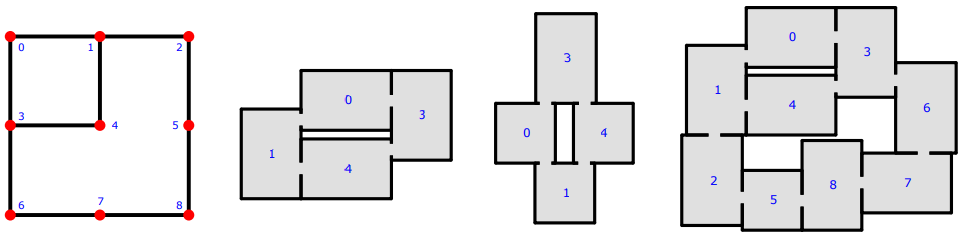
\includegraphics[width=0.9\textwidth]{obrazky/dung_simul_anneal.png}
    \caption{Ukázka generování dungeonu s~přímo propojenými místnostmi. Při generování byla využita metoda simulovaného žíhání. Nalevo je vstupní graf, uprostřed pak dvě možné varianty, jak vygenerovat geometrii menší smyčky v~grafu (řetězce), a vpravo je pak výsledný dungeon po propojení obou řetězců (smyček). Převzato z~\cite{lit:dung_simul_anneal}.}
    \label{img:dung_simul_anneal}
\end{figure}

%--------------------------------------------------------------

\subsection{Dělicí algoritmy}

%--------------------------------------------------------------

Dělicí algoritmy rozdělují 2D nebo 3D prostor na menší části, přičemž každý bod v~prostoru lze jednoznačně zařadit do jedné z~těchto menších částí (též nazývaných \textit{buňky}).
Dělicí algoritmy často pracují hierarchicky a jsou volány rekurzivně i na již vytvořené celky.
Výsledkem je stromová struktura částí, která je užitečná pro zpětné sestavování celku a také pro rychlé vyhledávání prvků.
Tyto vlastnosti se využívají zejména v~počítačové grafice.
\par
Nejznámějším dělicím algoritmem je metoda \textbf{binárního rozdělování prostoru} (BSP -- Binary Space Partitioning), která prostor rekurzivně dělí vždy na 2 části (ne nutně poloviny).
Vzniká tím tzv. binární strom nebo též BSP strom, kdy každý uzel má přesně dva potomky (viz obrázek \ref{img:bsp_first}).
\begin{figure}[hbt]
    \centering
    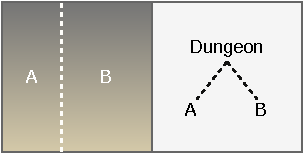
\includegraphics[width=0.6\textwidth]{obrazky/bsp_first.pdf}
    \caption{Ukázka první iterace binárního rozdělení prostoru (zde svisle), každá z~části A~a B je reprezentována jak v~prostoru, tak ve stromu.}
    \label{img:bsp_first}
\end{figure}
Tento algoritmus nachází využití také při generování dungeonů.
Protože prostor rozděluje na dvě části a žádná z~částí ve stromu se nikdy nepřekrývá, opakovaným rozdělováním lze vytvářet místnosti a ty zpětným vyhledáváním v~BSP stromu spojovat pomocí chodeb.
Tento přístup zajišťuje, že se místnosti nebudou překrývat, že budou všechny spojené a že bude celý dungeon průchodný.
Ve výsledných strukturách lze však vypozorovat jistá uspořádanost a některé společné vlastnosti, především fakt, že nikdy nedochází ke smyčkám.
\par
Na začátku algoritmu existuje pouze kořenový uzel, který představuje celou herní oblast.
Rekurzivním dělením herní oblasti poté vznikají podřazené uzly až po dosažení ukončovací podmínky (např. počet uzlů nebo minimální plocha části).
Nejčastěji tento algoritmus probíhá tak, že se daný prostor rozdělí nadrovinou\footnote{\textbf{Nadrovina} v~rozměru $n$ představuje podprostor v~rozměru $n-1$, například ve 3D je nadrovinou rovina, zatímco ve 2D je nadrovinou přímka.} rovnoběžnou s~jednou ze základních os.
Například pokud je vstupem čtverec, pak se rozdělí na dvě části pomocí jedné vodorovné nebo svislé čáry.
Algoritmus postupně dělí jednotlivé části, přičemž u~vzniklých částí rekurzivně volá dělicí funkci také.
Před rozdělením se vždy kontroluje, zda je vstup větší než minimální určená velikost.
Pokud není, funkce končí.
Jakmile rekurzivní volání dělicí funkce skončí, projdou se všechny uzly bez podřazených uzlů (listy) a v~oblasti, kterou reprezentují, se vyberou dva náhodné body (rohy místnosti).
U~těchto rohů se zkontroluje, zda jimi tvořená místnost splňuje požadavky na minimální velikost, případně se vyberou body nové nebo se stávající posunou směrem od středu.
Jakmile všechny části obsahují místnosti, dojde k~jejich propojování pomocí chodeb.
K~tomu je využit BSP strom.
Algoritmus projde všechny uzly stromu od nejnižších úrovní až po kořen, vybere vždy dva uzly se společným nadřazeným uzlem a mezi jejich místnostmi vytvoří chodbu.
Tímto postupným spojováním dojde k~propojení všech místností a celého dungeonu (viz obrázek \ref{img:bsp_second})\cite{lit:pcg_constructive_methods}.
\par
\begin{figure}[hbt]
    \centering
    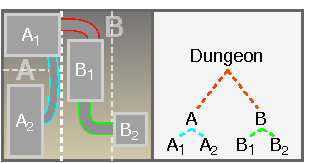
\includegraphics[width=0.8\textwidth]{obrazky/bsp_second.pdf}
    \caption{Jednoduchý dungeon vygenerovaný metodou BSP (vlevo). Dungeon se nejdříve rozdělí na dvě a poté na čtyři plochy, v~těch se vytvoří místností zaujímající určitou část plochy a poté se spojí místnosti reprezentované uzly v~BSP stromu (vpravo) tak, že se nejdříve propojí uzly $A_1$ a $A_2$, poté uzly $B_1$ a $B_2$ a poté se propojí jejich rodičovské uzly $A$ a $B$.} 
    \label{img:bsp_second}
\end{figure}
Metoda BSP je jednoduchý způsob, jak vytvářet hratelné dungeony.
Problémem je, že takto vzniklé dungeony nejsou příliš přizpůsobitelné a jsou poněkud omezené v~možnostech.
Dalším problémem je jejich poměrně velká uspořádanost a jednotvárnost, kterou lze z~části rozbít vytvářením menších místností v~určených částech (tím se však sníží jejich \uv{hustota}), případně upravit část algoritmu generujících místností tak, aby umožňovala místnosti různých tvarů nebo úplné vyplnění dostupného prostoru.

%--------------------------------------------------------------

\subsection{Generování pomocí agentů}

%--------------------------------------------------------------

Při procedurálním generování je důležitým požadavkem náhodnost, která zajistí jedinečný (ne repetitivní) obsah při každém spuštění generátoru -- tato náhodnost však nesmí způsobit ztrátu požadované míry uspořádanosti a spolehlivosti, nesmí docházet k~chybám a obsah musí dávat v~daném kontextu smysl.
Aby vygenerovaný obsah nevybočoval z~požadovaných hranic a nedocházelo k~nečekaným \uv{nehodám}, je nutné do algoritmů generátoru zahrnout faktor, který těmto situacím zabrání.
Možným řešením může být \textbf{generování pomocí agentů}, přičemž slovem agent se myslí autonomní prostředník s~určitou mírou naprogramované inteligence nebo též vzorců chování.
Agent dokáže snímat okolní prostředí, analyzovat jej a reagovat na něj v~rámci naprogramovaného chování.
\par
Autoři článku\cite{lit:agent_terrain} publikovaného v~jednom z~časopisů institutu IEEE v~roce 2010 využili agentů k~procedurálnímu generování 3D terénu.
Snažili se přitom, aby se jejich generátor vyznačoval náhodností, rychlostí a aby jej bylo možné jednoduchým způsobem ovládat a modifikovat.
Výsledný terén byl tvořen jednoduchou mřížkou bodů (v~práci autoři použili rozměry 512x512 bodů), které určovaly výškový profil a byly od sebe vzdálené přibližně 1~metr, výsledný vygenerovaný terén tak pokrýval oblast cca 0,25~km\textsuperscript{2}.
Ke generování použili různé druhy agentů, kteří měli různé úlohy, které se prováděly jedna po druhé (fáze generování):
\begin{enumerate}
    \item Pevnina -- tvorba základního tvaru pevniny, čímž přirozeně vzniká pobřežní čára, které může být poté obklopeno vodou
    \item Vyhlazování -- náhodné průchody, které průměrují výšku bodů v~okolí
    \item Pláže -- zarovnávání oblastí na pobřežní čáře
    \item Hory -- tvorba kopců, hor a pohoří
    \item Řeky -- eroze terénu vytvářející řeky směrem od hor k~pobřeží
\end{enumerate}
\begin{figure}[hbt]
    \centering
    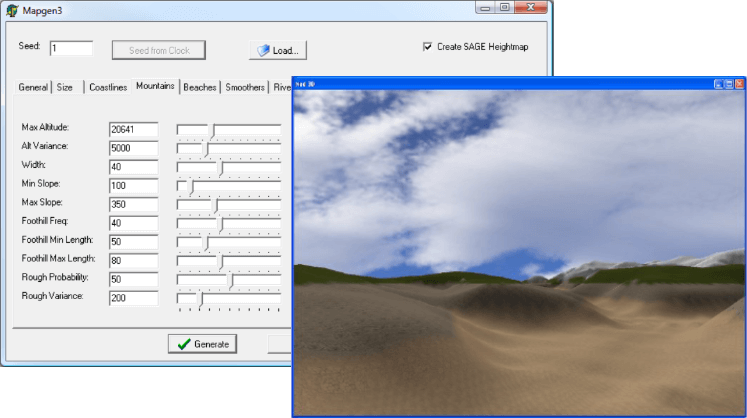
\includegraphics[width=0.85\textwidth]{obrazky/agent_terrain.png}
    \caption{Ukázka parametrů pro generování hor pomocí agentů (vlevo) a výsledný terén (vpravo), převzato z~\cite{lit:agent_terrain}.}
    \label{img:agent_terrain}
\end{figure}
\par
Všichni agenti mají společnou sadu vlastností: pracují asynchronně a souběžně, mají přehled o~výšce všech bodů na celé mapě a mohou je kdykoliv upravovat, protože jich však v~každé fázi pracuje více, podmínky kolem každého z~nich se mohou dynamicky měnit.
U~všech druhů agentů lze nastavit tzv. tokeny, které agenti spotřebovávají prováděním změn v~terénu.
Tokeny tedy určují jejich životnost a spolu s~počtem agentů jsou druhým parametrem, který má významný vliv na výsledek.
Agenti při své práci procházejí stanovenou částí terénu a upravují výškový profil podle požadovaných parametrů.
V~každé fázi je k~dispozici mnoho parametrů, které jsou zakomponovány jako proměnné do algoritmů.
\par
Agenty lze použít také pro generování dungeonů.
Pro takové případy se obvykle používá jediný agent, který prochází herní plochou, \uv{kope} tunely a vytváří místnosti.
Tím, že agent musí celý dungeon projít, je zajištěno, že jej bude moci projít i hráč.
Vzhled výsledného dungeonu pak závisí přímo na umělé inteligenci agenta a na informacích, které o~dungeonu má.
Problémem je, že je obtížné předpokládat, jaký vliv na výsledný vzhled dungeonu budou změny v~chování agenta mít.
Parametrem například může být, zda agent může protnout již existující chodby a místnosti.
Pokud ano, pak může být výsledná struktura chaotická a nevzhledná.
Pokud ne, pak se může agent zablokovat například v~rohu herní plochy a výsledný dungeon bude velmi malý.
\par
Nejjednodušším typem agenta je \uv{slepý} agent.
Tento agent začíná na libovolném místě v~dungeonu, odkud se pohybuje zcela náhodně bez ohledu na stav dungeonu, a při každém kroku mění dlaždici na jeho pozici na prostupnou (např. podlaha).
S~každým dalším krokem ve stejném směru se zvyšuje pravděpodobnost, že agent směr pohybu změní.
Po změně směru se pravděpodobnost změny směru nastaví na nulovou.
Obdobně funguje i vložení místnosti.
Při každém kroku se pravděpodobnost vložení místnosti zvýší a pokud dojde k~vložení místnosti (s~náhodnými rozměry a středem na pozici agenta), pravděpodobnost se nastaví na nulovou.
Tento přístup vede ke vzniku velmi chaotických dungeonů s~překrývajícími se místnostmi a slepými uličkami (viz obrázek \ref{img:agent_dungeon} vlevo).
\begin{figure}[hbt]
    \centering
    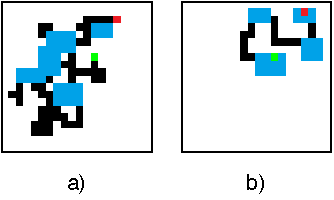
\includegraphics[width=0.5\textwidth]{obrazky/agent_dungeon.pdf}
    \caption{Ukázka dungeonů vytvořených pomocí agentů. Zeleně je označen počátek, červeně je označen konec. Dungeon vlevo vznikl pomocí \uv{slepého} agenta a obsahuje překrývající se místnosti a slepé uličky. Dungeon vpravo vznikl pomocí \uv{informovaného} agenta a v~tomto případě skončil předčasně.}
    \label{img:agent_dungeon}
\end{figure}
\par
Dalším pokročilejším, ale přesto jednoduchým typem agenta je \uv{informovaný} agent.
Tento agent má informace o~místnostech a chodbách a snaží se je pokládat tak, aby nedocházelo k~jejich průniku.
To zajišťuje tím, že když má položit místnost nebo chodbu, hlídá, aby tím nevznikla kolize.
Pokud by ke kolizi došlo, zkusí místnost a chodbu s~jinými rozměry (v~rámci minimální a maximální definované velikosti).
Agent se do místnosti nebo na konec chodby přesune až po jejich úspěšném vytvoření.
Pokud ke kolizi dochází u~všech možných kombinací velikostí, algoritmus končí.
Tento agent vytváří dungeony, které jsou průchodné, nekříží se, ale jsou velmi lineární.
Navíc může snadno dojít k~tomu, že se agentovi nepodaří vložit žádnou místnost ani chodbu, a z~tohoto důvodu algoritmus skončí, ačkoliv velká část herní plochy může zůstat nevyužita (viz obrázek \ref{img:agent_dungeon} vpravo).
\par
Ani jeden ze zmiňovaných přístupu není připraven pro použití v~praxi.
První přístup vytváří příliš chaotickou strukturu s~překrývajícími se místnostmi, druhý přístup zase může způsobit předčasné ukončení algoritmu.
Přidávání dalších podmínek a \uv{inteligence} k~agentovi může tyto problémy vyřešit, faktem však zůstává, že tvorba dungeonů tímto způsobem vyžaduje značné množství úsilí, času a experimentování s~nepříliš jasnými výsledky.
Tato metoda je tedy vhodná především v~situacích, kdy je potřeba dosáhnout méně strukturované až chaotické podoby (např. jeskyně), nebo pokud je hlavní požadovanou vlastností nepředvídatelnost výsledného dungeonu\cite{lit:pcg_constructive_methods}.

%--------------------------------------------------------------

\chapter{Současná řešení generování dungeonů}
\label{ch:soucasnost} % 3

%--------------------------------------------------------------

Tato kapitola obsahuje náhled na existující, praktická řešení generování dungeonů.
V~první části jsou představeny existující hry, které pomocí některých z~výše uvedených technik vytvářejí skutečné a hratelné dungeony.
Druhá část se pak na již existující řešení dívá z~perspektivy vývojářské~--~jsou prezentovány knihovny, které vývojářům umožňují dungeony generovat.

%--------------------------------------------------------------

\section{Generování dungeonů v~existujících hrách}

%--------------------------------------------------------------

Tato část popisuje dungeony v~některých známých existujících hrách.
Ne vždy je jasné, jaké techniky vývojáři pro generování dungeonů použili.
Zejména v~komerčních hrách bez otevřeného zdrojového kódu lze pouze hádat, jak hra vnitřně funguje.
Nicméně i samotným pozorováním topologické a geometrické stavby těchto úrovní si lze udělat dobrý obrázek o~tom, jak generátory fungují.
Analýza těchto herních úrovní může navíc sloužit jako předloha pro požadavky na vytvářenou knihovnu.

%--------------------------------------------------------------

\subsection{Rogue (1980)}

%--------------------------------------------------------------

Rogue je počítačová hra, která dala vzniknout žánru tzv. Roguelike her.
Vyvinuli ji Michael Toy, Glenn Wichman a Ken Arnold pro Unixové systémy a vydali ji v~roce 1980.
Hra si rychle získala srdce spousty hráčů a programátorů, protože obsahovala tehdy revoluční (ale ne úplně první) procedurálně generované dungeony, ve kterých museli hráči bojovat proti příšerám, získávat lepší vybavení a vylepšovat svou postavu.
Hra disponovala jednoduchou ASCII grafikou (viz obrázek \ref{img:rogue_gameplay}).
Pro hru bylo nutné vytvořit efektivní algoritmus generování dungeonů.
Dungeony ve hře \textit{Rogue} jsou tvořeny jednoduchými obdélníkovými místnostmi, které jsou propojeny chodbami.
Dungeon bylo nutné vygenerovat ve velmi omezeném prostoru, protože herní plochu nebylo možné rolovat -- vždy se zobrazovala celá úroveň a ta byla omezena staticky daným množstvím možných ASCII znaků na výšku a na šířku.
\begin{figure}[hbt]
    \centering
    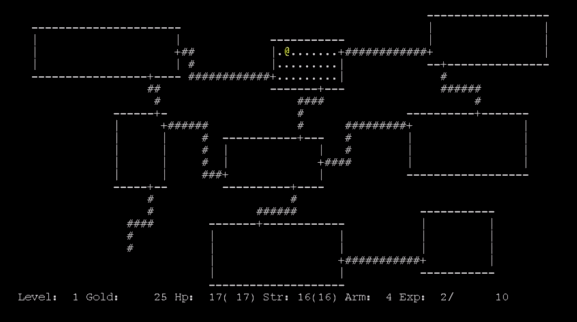
\includegraphics[width=0.7\textwidth]{obrazky/rogue_gameplay.png}
    \caption{Ukázka ze hry \textit{Rogue}, místnosti a chodby dungeonu jsou tvořeny ASCII grafikou.}
    \label{img:rogue_gameplay}
\end{figure}
\par
Algoritmus ve hře je poměrně jednoduchý.
Celá herní plocha se rozdělí na mřížku 3x3 buněk.
Každá buňka představuje jednu místnost, která může mít v~rámci prostoru buňky náhodnou velikost.
Místnosti obsahují informaci o~tom, zda jsou připojeny k~alespoň jedné jiné místnosti, a seznam místností, ke kterým jsou připojeny.
Algoritmus začíná náhodným výběrem jedné začáteční buňky, ve které se hráč na začátku úrovně objeví.
Následně se vybere sousední nepropojená místnost, vytvoří se mezi nimi chodba a začáteční místnost se označí jako propojená.
Algoritmus se poté opakuje u~této vybrané sousední místnosti, tedy místnost se propojí s~jinou sousední nepropojenou místností a označí se jako propojená.
Takto algoritmus v~cyklu pokračuje, až dokud nelze vybrat žádnou sousední místnost, protože jsou všechny sousední místnosti propojeny.
Následně algoritmus projde všechny zbylé nepropojené místnosti a propojí je s~některou ze sousedních propojených místností.
Nyní má každá místnost minimálně jedno propojení.
Do naposledy propojené místnosti se přidá schodiště vedoucí do další úrovně -- tato místnost je obvykle nejdále od začáteční místnosti.
Algoritmus nakonec může vytvořit další náhodná propojení mezi místnostmi.
V~některých úrovních může dojít k~tomu, že se v~buňce mřížky místnost nevytvoří a tato buňka se použije pouze jako prodloužená chodba.
Díky tomu nejsou výsledné dungeony tak jednotvárné\cite{lit:rogue}.
\par
Uvedený algoritmus je velmi jednoduchý, rychlý a je vždy úspěšný.
Takto vytvořený dungeon je zcela průchodný.
Nevýhodou je omezený počet místností, rozměry mřížky je sice možné zvětšit, ale dungeon zůstane stále velmi stereotypní a příliš uspořádaný.

%--------------------------------------------------------------

\subsection{Diablo 1 (1996)}

%--------------------------------------------------------------

Diablo 1 je hra vytvořená firmou Blizzard Entertainment a vydaná v~roce 1996.
Tato hra se stala velmi populární a dodnes je považována za důležitého předchůdce moderních her na hrdiny s~dungeony.
Hráč v~této hře začíná v~bezpečné statické úrovni, ve vesničce Tristram, odkud provádí výpravy do podzemních, náhodně generovaných úrovní (dungeonů).
Hra obsahuje těchto úrovní celkem 16 ve čtyřech různých prostředích, z~nichž každé je generováno jiným způsobem.
Jako většina komerčních titulů neměla hra otevřený zdrojový kód a proto se fanoušci mohli jen dohadovat, jakým způsobem hra úrovně generovala.
V~roce 2018 programátor, který vystupuje pod přezdívkou GalaXyHaXz, zpětným inženýrstvím ladicích informací a symbolických odkazů omylem ponechaných v~japonské verzi hry rekonstruoval přibližný původní zdrojový kód hry a spolu s~dalšími autory jej vydali pod názvem Devilution\footnote{Původní projekt Devilution~--~\url{https://github.com/diasurgical/devilution}}.
Poté vznikl projekt DevilutionX\footnote{Verze projektu Devilution pro moderní OS~--~\url{https://github.com/diasurgical/devilutionX}}, který si klade za cíl přizpůsobit hru moderním operačním systémům a poskytnout fanouškům prostředky pro další modifikace této kultovní hry.
Tyto verze ale stále slouží pouze jako nadstavby pro původní hru.
Bez vlastnictví původní hry a jejích zdrojů (grafika, zvuky, animace atd.) nelze tyto rekonstruované hry spustit.
\begin{figure}[t]
    \centering
    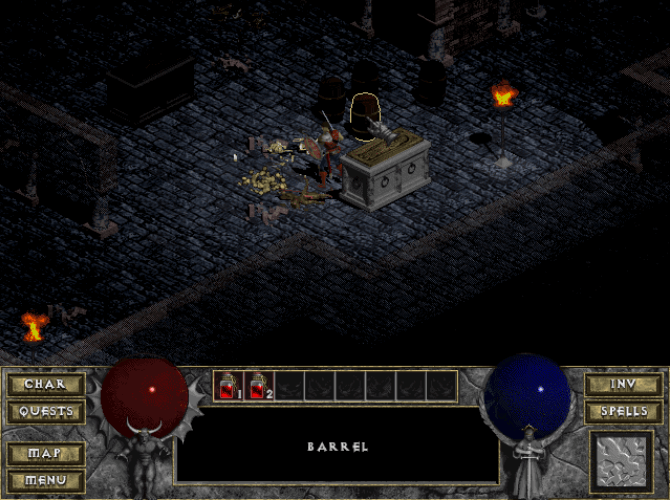
\includegraphics[width=0.8\textwidth]{obrazky/diablo_1_gameplay.png}
    \caption{Ukázka ze hry \textit{Diablo 1}.}
    \label{img:diablo_1_gameplay}
\end{figure}
\par
S~možností nahlédnout do zdrojového kódu už nic nebránilo tomu, aby fanoušci začali zjišťovat, jaké vnitřní mechanismy hra využívala.
V~červenci roku 2019 se na webovém blogu objevil článek\cite{lit:diablo_1}, který celkem podrobně analyzuje chování procedurálního generátoru úrovní v~Diablu 1.
\par
Jak již bylo zmíněno, úrovně Diabla 1 se dělí do čtyř prostředí a hráč se s~nimi setkává postupně s~tím, jak sestupuje do níže položených úrovní.
Jsou to: \textbf{kostel}, \textbf{katakomby}, \textbf{jeskyně} a \textbf{peklo}.
Ačkoliv každé prostředí má svá specifika, podle kterých byl generátor pro to či ono prostředí přizpůsoben, mají i mnoho společného.
Každá úroveň se skládá ze 40x40 dlaždic, přičemž každá dlaždice se poté ještě dělí na 4 části, které slouží pro jemnější grafické detaily a určení průchodnosti postavou hráče.
Generátor úrovní pracuje ve dvou fázích:
\begin{itemize}
    \item Předběžný dungeon~--~Na konci této fáze je vytvořena kostra dungeonu.
    Veškerý prostor je rozdělen do jednoho ze dvou stavů~--~průchozí (stěna) nebo neprůchozí (podlaha).
    Na konci této fáze dungeon navíc obsahuje dveře a další vysokoúrovňové prvky.
    \item Konečný dungeon~--~V~této fázi generátor řeší rozmístění grafických prvků, dodává do úrovně další stěny, sloupce, předem připravené části a další detaily.
\end{itemize}
Samotná tvorba místností a chodeb probíhá dvěma velmi odlišnými způsoby.
\par
\textbf{První metoda} se používá pro úrovně v~prostředí kostela, jeskyně a pekla (pouze s~mírnými variacemi, jejichž výsledkem je, že každé další prostředí je otevřenější než to předchozí).
Celý proces začíná vyplněním herní plochy neprůchozí stěnou a tvorbou místností na této ploše.
Místnost je čtvercová nebo mírně obdélníková konstrukce tvořena podlahou a stěnami na okrajích.
V~prostředí jeskyní pak má místnost nepravidelné okraje, generátor 50~\% stěn nahradí za podlahu.
V~prostředí kostela se vkládají dvě velké místnosti propojené širokou chodbou se sloupy, v~jeskyni a pekle pouze jedna místnost.
V~pekle je pak na okraji této hlavní místnosti vytvořena chodba táhnoucí se napříč a propojená se zbytkem místnosti.
\par
Generování dalších místností probíhá voláním rekurzivní funkce, která napojuje další menší místnosti na okraje stávajících místností (pokud je tam dostatek volného místa).
Průchodnost celého dungeonu je vždy zajištěna tím, že místnosti doléhají přímo na hranu, čímž dochází k~jejich přímému spojení a odstranění této hrany.
V~prostředí kostela se tato funkce volá na samotnou místnost, ve které vybere náhodně osu X nebo osu Y a na okrajích místností po vybrané ose vytvoří dvě místnosti.
Vytvořené místnosti se zarovnají se středy hran.
Následně je funkce rekurzivně volána i pro nově vzniklé místnosti, pouze se použije osa opačná.
Rekurzivní volání končí, jakmile není místo k~vytváření nových místností.
Stejný postup se používá i v~prostředí pekla, místnosti však mají fixní velikost a generuje se jich pouze omezený počet daný součtem podlahových dlaždic.
Tyto vygenerované místnosti se poté zrcadlově kopírují~--~svisle i vodorovně~--~díky čemuž jsou úrovně v~pekle velmi symetrické.
V~prostředí jeskyní se funkce pro generování místností volá pro každou hranu místnosti.
Místnosti vytvořené na hranách nejsou nijak zarovnávány, jejich umístění je náhodné, jsou však daleko menší, čímž je celá jeskynní úroveň členitější, ale ve výsledku otevřenější.
V~jeskynních úrovních mohou místnosti vytvářet také smyčky a napojovat se na již existující předchozí místnosti, což jen podporuje jejich otevřenost.
\par
Generátor v~prostředí kostela a v~prostředí jeskyní poté dodatečně vytváří stěny, které vycházejí z~jedné stěny a končí u~jiné.
V~kostele se stěny táhnou vždy od rohu podél stěny do volného prostoru až k~další stěně kde končí.
Díky tomu je prostředí kostela velmi strukturované.
Stěny jsou poté v~25\,\% případů nahrazeny průchodným sloupořadím, v~25\,\% případů mřížemi a jinak zůstávají stěnami.
Do těchto stěn a mříží jsou poté přidány dveře nebo oblouky, které zajišťují průchodnost po celém dungeonu.
V~prostředí jeskyní nemusí generované stěny vycházet přímo z~rohů, ale z~jakéhokoliv místa jiné stěny.
I~tyto stěny jsou poté zprůchodněny dveřmi.
\par
Jeskynní úroveň je dále specifická tím, že se úroveň \uv{začišťuje} algoritmem pro erozi.
Osamostatněné stěny uprostřed volného prostoru jsou odstraněny, u~dlouhých rovných stěn na okrajích se vytváří členitější struktura tím, že se 50\,\% stěn nahradí za podlahu.
Větší celky stěn obklopené ze všech stran podlahou jsou nahrazeny za lávu (fakticky se jedná o~stěnu jen s~jinou texturou) a z~těchto lávových jezer poté proudí řeky až ke stěnám.
Aby řeky nenarušily průchodnost úrovně, generátor přes ně vytváří na vhodných místech mosty.
\par
\textbf{Druhá metoda} se používá výhradně pro katakomby a je velmi speciální.
Generátor katakomb si ukládá veškeré dlaždice do ASCII mapy (vývojáři společnosti Blizzard byli inspirování žánrem Roguelike, viz část \ref{ssec:historie_dungeonu_a_roguelike}).
Toto řešení navíc nevyžaduje žádné pokročilé struktury pro uchování dat.
Prázdné políčko (\texttt{' '}) znamená neprůchozí dlaždici.
Na začátku algoritmu je zavolána rekurzivní funkce, které je předána jako vstup celá plocha úrovně bez okrajů.
Tato funkce má za úkol vygenerovat místnosti ve vstupní oblasti, přičemž si uchovává referenci na místnost, která ji zavolala (na začátku algoritmu null).
Nová místnost má náhodnou velikost (přizpůsobenou velikosti vstupní oblasti) a její pozice v~rámci vstupní oblasti je také náhodná.
Místnost se do ASCII mapy zakreslí následovně: okraje místnosti (stěny) se zapíší jako \texttt{'\#'}, dlaždice podlah se zapíší jako \texttt{'.'} a rohy místnosti se zapíší písmeny \texttt{'A', 'B', 'C', 'E'}.
Pokud není reference na volající místnost null, generátor na nejbližších stranách volající a nové místnosti vybere dvě náhodné rovnoběžné dlaždice stěn a uloží je do seznamu chodeb pro pozdější využití.
Zbytek vstupní oblasti se rozdělí na čtyři obdélníkové oblasti, jejichž velikost se zmenší o~2 (aby vznikla mezi místnostmi mezera) a poté se pro ně zavolá rekurzivní funkce pro tvorbu místností s~referencí na právě vygenerovanou místnost.
Po dokončení rekurzivních funkcí (které skončí, jakmile už nebude prostor pro nové místnosti) je nutné mezi vygenerovanými místnostmi vytvořit chodby.
Ty vzniknou přímým propojením dvojic stěn uložených dříve.
Chodbám se určí náhodná šířka 1 až 3 dlaždice a zarovnají se pomocí rohů propojovaných místností.
Pokud chodba protne stěnu (\texttt{'\#'}), znak se změní na \texttt{'D'} (door), pokud protne neprůchozí dlaždici (\texttt{' '}), znak se změní na \texttt{','}, což označuje chodbu samotnou.
Tento mezi-zápis umožňuje křížení chodeb.
Po zakreslení chodeb se rohy (\texttt{'A', 'B', 'C', 'E'}) změní na stěny (\texttt{'\#'}), neprůchozí dlaždice (\texttt{' '}) vedle chodeb (\texttt{','}) se změní také na stěny (\texttt{'\#'}) a samotné znaky chodeb (\texttt{','}) se nakonec nahradí podlahou (\texttt{'.'}).
Na závěr se spustí algoritmus, který vyhledá nevyužitý prostor na mapě a vyplní jej protáhnutím existujících místností, případně vytvořením nových místností.
\par
Generátor Diabla 1 kromě generování místností a chodeb provádí mnoho procedur, bez kterých by nebyly herní úrovně kompletní.
Následuje jejich stručný výčet.
\subsubsection{Předem připravené části}
Hra obsahuje několik předem připravených částí, které slouží především pro úkoly v~té dané úrovni.
Tyto předem připravené části generátor jednoduše vloží podle určitých parametrů (v~závislosti na prostředí dané úrovně).
Může se jednat například o~podstavec s~knihou a svíčkami okolo nebo o~místnost s~obtížným protivníkem a specifickým grafickým zpracováním.
\begin{figure}[hbt]
    \centering
    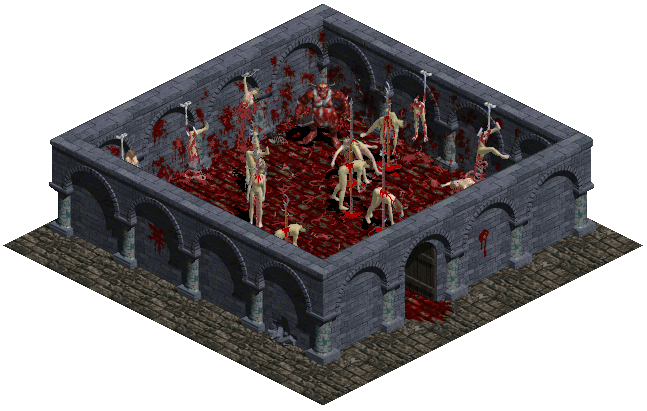
\includegraphics[width=0.7\textwidth]{obrazky/diablo_1_butcher.png}
    \caption{Typická předem připravená část ve hře \textit{Diablo 1}~--~řezníkovo doupě. Místnost je pokaždé naprosto stejná. Převzato z~\cite{lit:diablo_1}.}
    \label{img:diablo_1_butcher}
\end{figure}
\subsubsection{Mini-části}
Každá úroveň má připraveny desítky tzv. mini-částí, které generátor do úrovně vkládá na základě různých pravidel.
Tato pravidla mohou zahrnovat např. výskyt určitých prvků v~úrovni nebo vložení na základě pravděpodobnosti.
Mini-části slouží k~dekorování úrovní (např. výbušné sudy, světla, kaluže krve), k~opravám chyb vzniklých generováním (je jednodušší tyto chyby opravovat v~postprodukci než je opravovat v~hlavní fázi generování) nebo třeba ke vkládání schodišť propojujících úrovně.
\subsubsection{Speciální místnosti}
Ve hře se vyskytují místnosti, které mají určité speciální zaměření.
Tyto místnosti mají stanovené optimální rozměry a úrovně, ve kterých se mohou vygenerovat.
Může se jednat například o~knihovnu, ve které hráč nalezne vždy minimálně jeden svitek, nebo o~místnost plnou příšer.
V~prostředí kostela generátor tyto místnosti vytváří tak, že si vybere nějakou z~již existujících místností a tu přepracuje.
V~dalších prostředích je jednoduše vkládá do volného prostoru.
\subsubsection{Kontrolní mechanismy}
Generování úrovní se neobejde bez kontrolních mechanismů, které zjistí, zda vygenerovaná úroveň splňuje požadované parametry.
V~úrovních se kontroluje především průchodnost dungeonu napříč, zda se podařilo vložit předem připravenou část pro úkol dané úrovně a zda došlo k~vygenerování dostatečného počtu průchozích dlaždic.
Pokud některá z~těchto kontrol selže, generování probíhá celé od začátku.
\begin{figure}[hbt]
    \centering
    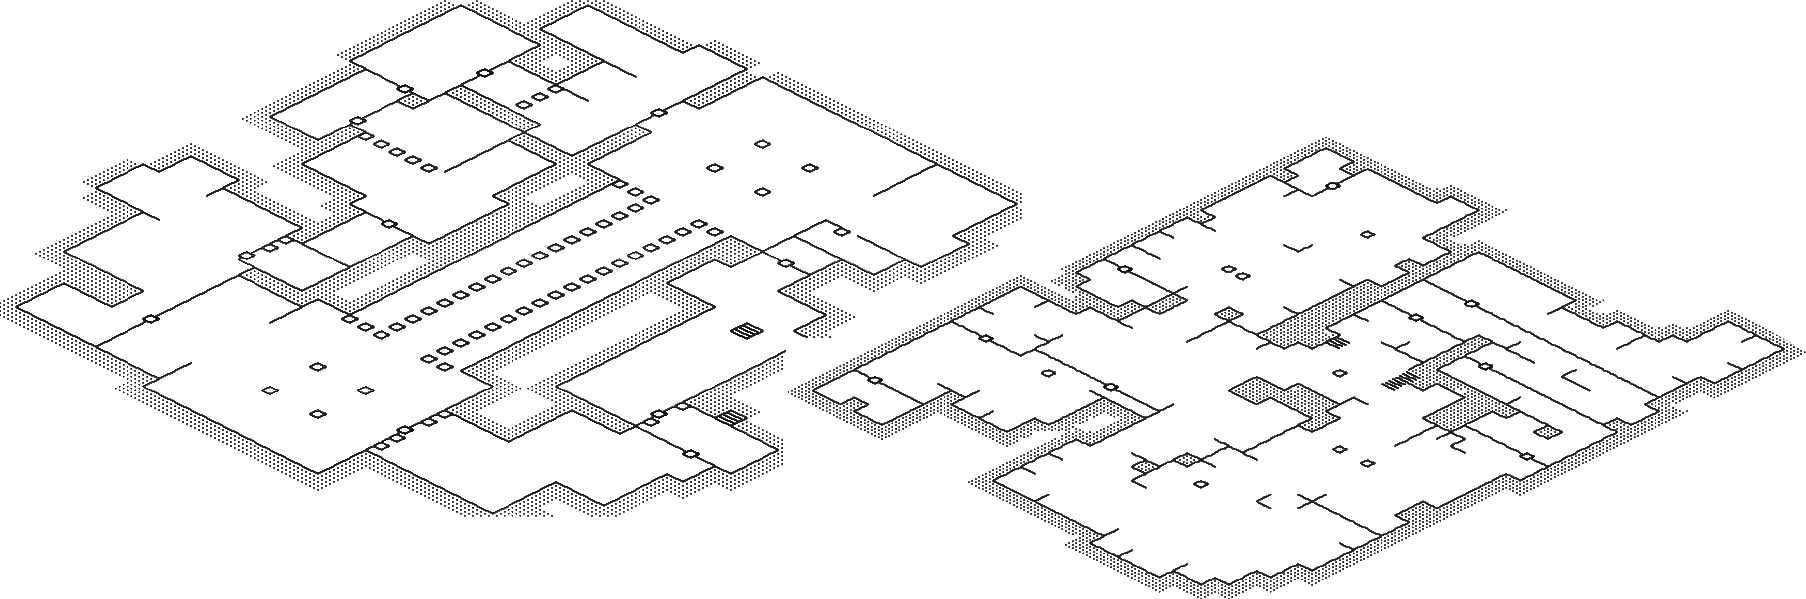
\includegraphics[width=1.0\textwidth]{obrazky/diablo_1_maps.png}
    \caption{Ukázka struktur vygenerovaných úrovní ve hře \textit{Diablo 1}, kostel (vlevo) je mnohem uspořádanější, zatímco jeskyně (vpravo) má více entropický charakter, převzato z~\cite{lit:diablo_1}.}
    \label{img:diablo_1_maps}
\end{figure}

%--------------------------------------------------------------

\subsection{Don't Starve (2013)}

%--------------------------------------------------------------

Don't Starve je počítačová hra vydaná v~roce 2013 kanadskou společností Klei Entertainment.
Jedná se o~hru žánru survival (boj o~přežití), ve které se hráč ujímá role protagonisty Wilsona, vědce, který se za podivných okolností objeví v~tajemném a neprobádaném světě.
Tento svět je náhodně generovaný a hráč v~něm má volné pole působnosti -- může vyrábět různé předměty, objevovat rozličná místa a musí se pokusit přežít (režim sandbox -- pískoviště).
V~tomto světě se nachází předmět, který hráče přemístí do režimu dobrodružství.
V~tomto režimu má hráč jediný cíl -- zjistit, co se mu stalo a proč a porazit antagonistu Maxwella.
V~režimu dobrodružství hráč postupně prochází pět náhodně generovaných světů, přičemž v~každém z~nich začíná téměř od nuly.
Smrt v~kterémkoliv světě znamená, že se hráč přesune do úplně prvního světa a ztratí veškerý postup.
Tento mechanismus \uv{trvalé smrti} se nápadně podobá žánru Roguelike.
\par
\begin{figure}[hbt]
    \centering
    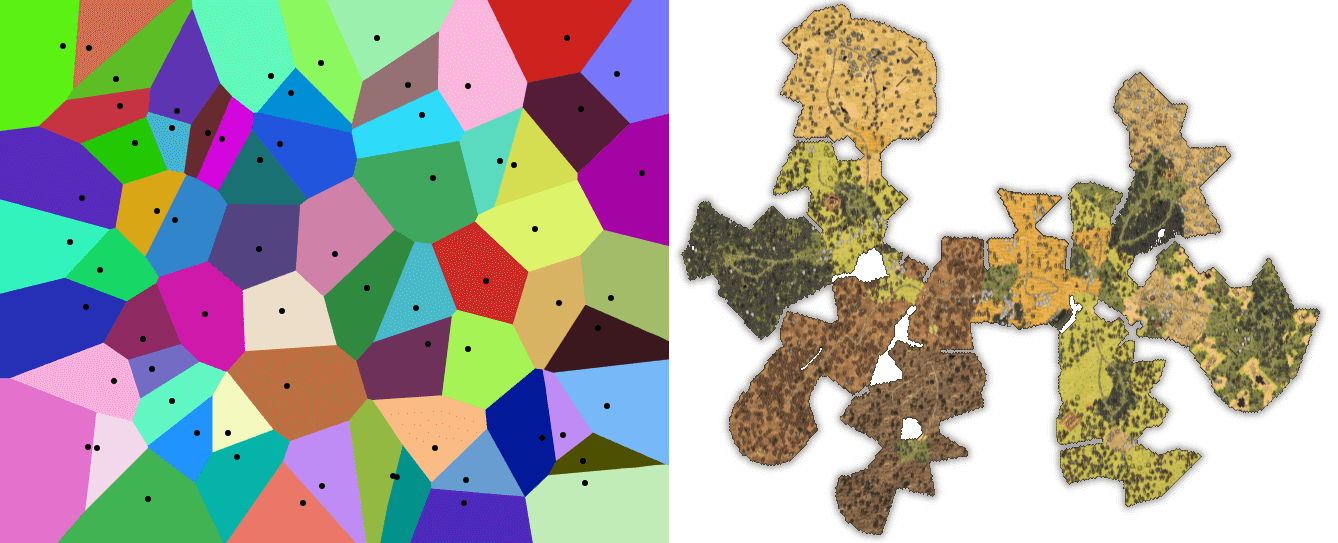
\includegraphics[width=1.0\textwidth]{obrazky/dont_starve_map.png}
    \caption{Náhodný Voroného diagram (vlevo) a ukázka mapy ze hry \textit{Don't Starve} vytvořené pomocí Voroného diagramu (vpravo). Herní plocha se rozdělí na menší části a těm se poté přiřadí specifický účel a vzhled. Části bez účelu budou zahozeny.}
    \label{img:dont_starve_map}
\end{figure}
Jak již bylo zmíněno, světy v~Don't Starve jsou procedurálně generované.
Ačkoliv je svět otevřený, lze jej interpretovat jako síť propojených místností a tedy i jako dungeon.
Jejich fyzická geometrická struktura je vytvořena na základě Voroného diagramu\footnote{\textbf{Voroného diagram} je kolekce oblastí vzniklých dělením roviny na základě vzdáleností k~dané diskrétní množině bodů.} (viz obrázek \ref{img:dont_starve_map}).
Světy občas mohou obsahovat vchody do dalších světů.
Každý svět má přiřazen motiv, který určuje, jak bude vypadat terén a jaké se ve světě vygenerují úlohy, předměty, nepřátelé a další prvky.
Místnosti světa jako takové se generují na základě úloh, které hráč musí vykonat.
Každá úloha obsahuje seznam tzv. zámků a klíčů, které abstraktně reprezentují posloupnost úkonů v~dané úloze.
Při generování se pro každou úlohu vytvářejí uzly místností (s~případnými klíči nebo zámky), které se zařazují podle určitých pravidel do grafu (který je ze začátku lineární, poté může utvářet i smyčky).
Úlohy se svými místnostmi se poté zařazují do stromové struktury podle toho, jaké klíče a zámky obsahují.
Kontroluje se přitom, aby nedošlo k~situaci, kdy by se hráč ocitl v~bezvýchodné situaci.
Graf může být na náhodných místech propojen, což usnadňuje průchod, a případně mohou být vloženy teleportační prvky, které fakticky graf spojují také.
Nakonec je pro takto utvořený graf vytvořena geometrická podoba úrovně a přiřazena grafika\cite{lit:dont_starve}.
\par
Generátor úrovní ve hře Don't Starve ukazuje, že při vytváření úrovně zohledňující hráčův postup může být výhodné nejdříve vygenerovat abstraktní graf, kterému lze poté pomocí některé metody (například Voroného diagramu) přiřadit geometrickou podobu.

%--------------------------------------------------------------

\section{Dostupné knihovny pro generování dungeonů}
\label{sec:dostupne_knihovny}

%--------------------------------------------------------------

Tato část popisuje některé existující knihovny pro generování dungeonů.
U~každé z~nich je provedena analýza základních funkcí, vstupů, výstupů, případně také technik, které používají.
Průzkum existujících knihoven může poskytnout představu o~tom, kterým směrem by se měla nová knihovna ubírat.

%--------------------------------------------------------------

\subsection{DungeonGenerator (jongallant)}
\label{ssec:dungeongenerator_jongallant}

%--------------------------------------------------------------

Zajímavý generátor pro systém Unity, který při tvorbě dungeonů využívá fyzikálního systému, algoritmu pro normální rozdělení v~kružnici, delaunayovy triangulace a vyhledávání minimální kostry grafu\cite{lit:lib_adn}.\medskip

\noindent Projekt na GitHubu: \url{https://github.com/jongallant/DungeonGenerator}\medskip

Tato knihovna má jediný účel: vygenerovat dungeon skládající se z~místností a chodeb, přičemž i samotné chodby mohou být tvořeny vedlejšími místnostmi.
Knihovna je určena pro použití v~systému Unity a je napsána v~jazyce C\#.
Dostupnými \textbf{vstupními parametry} knihovny jsou:
\begin{itemize}
    \item Počet místností
    \item Poloměr kružnice, do které budou místnosti rovnoměrně vkládány (a následně pomocí fyzikálního systému rozprostřeny)
    \item Podíl hlavních místností
    \item Množství dodatečných propojení mezi místnostmi
\end{itemize}
Parametry jsou pevně zapsány v~kódu a je nutné jejich hodnotu upravovat tam.
To vyžaduje alespoň obecný přehled nad vnitřní strukturou knihovny.
Knihovna nenabízí konfigurační soubor.
\textbf{Výstupem knihovny} je:
\begin{itemize}
    \item Seznam místností a jejich vlastností (pozice, rozměry)
    \item Seznam vytvořených chodeb mezi místnostmi
    \item 2D mřížka obsahující místnosti a chodby ve formě dlaždic
    \item Rastrový obrázek dungeonu.
\end{itemize}
Generátor lze spustit například přetažením skriptu \texttt{DungeonGenerator.cs} na příslušný \texttt{GameObject} Unity scény a následným stiskem tlačítka \texttt{Play}.
Třída \texttt{DungeonGenerator} je potomkem standardní Unity třídy \texttt{MonoBehaviour}, která zajistí její spuštění.
Po spuštění se nejdříve zavolá metoda \texttt{RoomGenerator.Generate}, která vytváří zadaný počet místností s~náhodnými rozměry a vektorovou reprezentaci rovnoměrně na kružnici o~zadaném poloměru.
Největší místnosti se určí jako hlavní (ty jsou vždy součástí výsledného dungeonu a tvoří body kostry grafu), ostatní jako vedlejší (ty jsou součástí dungeonu jen pokud je protíná některá z~chodeb mezi hlavními místnostmi).
\begin{figure}[t]
    \centering
    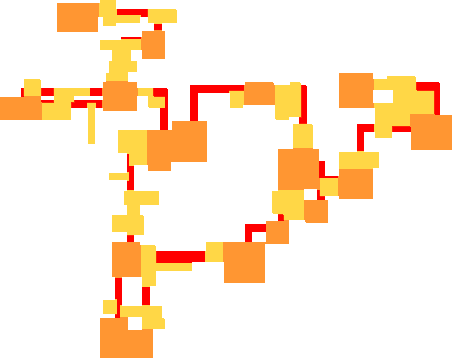
\includegraphics[width=0.6\textwidth]{obrazky/dunglib_jongallant.png}
    \caption{Ukázka dungeonu vygenerovaného pomocí knihovny \href{https://github.com/jongallant/DungeonGenerator}{DungeonGenerator (jongallant)}. Oranžově jsou vyobrazeny hlavní místnosti, žlutě vedlejší místnosti a červeně chodby.}
    \label{img:dunglib_jongallant}
\end{figure}
Všechny místnosti jsou asociovány s~fyzikálními objekty Unity \texttt{Rigidbody2D}, které zajišťují, že se při překrývání rozpínají a odsunují od sebe.
Fyzikální systém Unity zajistí, že se místnosti rozprostřou po herní ploše a nebudou se překrývat.
Tento proces je nepředvídatelný a zajišťuje unikátní ráz dungeonu při každém vygenerování.
Jakmile se místnosti ustálí, u~všech hlavních místností se vyhledají středy a ty se použijí do algoritmu delaunayovy triangulace, který mezi nimi vytvoří trojúhelníkovou mřížku.
Tato mřížka se poté převede na graf a pro takto vzniklý graf se vypočítá minimální kostra.
Ta zajistí, že všechny hlavní místnosti budou v~rámci dungeonu dosažitelné, ale nebudou všechny vzájemně propojené.
Protože je minimální kostra grafu lineární struktura bez smyček, do grafu se náhodně přidají dodatečná propojení.
Hlavní místnosti se poté propojí chodbami.
V~tomto případě se používají tři typy chodeb: rovné vodorovné, rovné svislé nebo chodby ve tvaru písmene L.
Chodba samotná je také fyzikálním objektem a pokud protne fyzikální objekt vedlejší místnosti, vedlejší místnost se stane součástí dungeonu.
Ostatní vedlejší místnosti se zahodí.
Následně se vytvoří 2D mřížka a procesem podobný rasterizaci se matematicky zapsané místnosti a propojení převedou na dvourozměrné pole dlaždic, z~nichž každá je reprezentována celým číslem: 0 = prázdné místo, 1 = propojení, 2 = stěna.
Místnosti a chodby tak v~dungeonu získají prostorovou charakteristiku.
Knihovna nakonec vygeneruje také rastrový obrázek vytvořeného dungeonu.
\par
Knihovna se nepoužívá příliš intuitivně, protože neobsahuje žádné veřejné rozhraní.
Uživatel musí upravovat přímo vnitřní parametry a vyextrahovat si výstup sám.
Její vstupní parametry jsou navíc velmi omezené.
Kladnou stránkou je fakt, že knihovna vytváří jak matematickou (vektorovou) reprezentaci místností a chodeb, tak 2D mřížku a dokonce i obrázek, který může sloužit jako mapa.
Místnosti jsou však obecné a je na vývojáři, aby jim dal jejich funkci až poté.
Generování nelze přizpůsobit potřebám hry a herních prvků (například nelze určit, že jedna místnost má být počáteční a druhá koncová a tyto dvě od sebe při generování co nejvíce vzdálit).
Knihovna je navíc omezena pouze na využití v~systému Unity, protože využívá jeho mechanismů.

%--------------------------------------------------------------

\subsection{Rot Web API (MattMcFarland)}
\label{ssec:rotwebapi}

%--------------------------------------------------------------

Webová služba vytvořená v~systému Node.js, která nabízí rozhraní pro tvorbu Roguelike map, bludišť, jeskyní pomocí celulárních automatů a dungeonů pomocí agentů.
Funguje jako webový server, který zpracovává HTTP GET požadavky a odpovídá JSON strukturami.\medskip

\noindent Projekt na GitHubu: \url{https://github.com/MattMcFarland/rot-web-api}\medskip

Knihovnu lze nainstalovat pomocí správce balíků \textit{npm} příkazem \texttt{npm install} a poté ji lze spustit příkazem \texttt{npm start}.
Knihovna nabízí několik typů generátorů, z~nichž každý je dostupný prostřednictvím svého rozhraní.
Každý generátor lze zavolat příslušným požadavkem HTTP GET na adresu webové služby s~příslušnými parametry.
Například generátor \texttt{Rogue} nabízí parametry \textit{width}, \textit{height}, \textit{roomWidth} a \textit{roomHeight} a lze jej například zavolat tímto způsobem:\medskip

\noindent \begin{texttt}http://localhost:8080/api/rogue?width=80\&height=25\&roomWidth=10\&roomHeight=10\end{texttt}\medskip

Po obdržení požadavku server vygeneruje Roguelike dungeon a zašle zpět odpověď ve formátu JSON (viz obrázek \ref{img:dunglib_mattmcfarland}).
\begin{figure}[hbt]
    \centering
    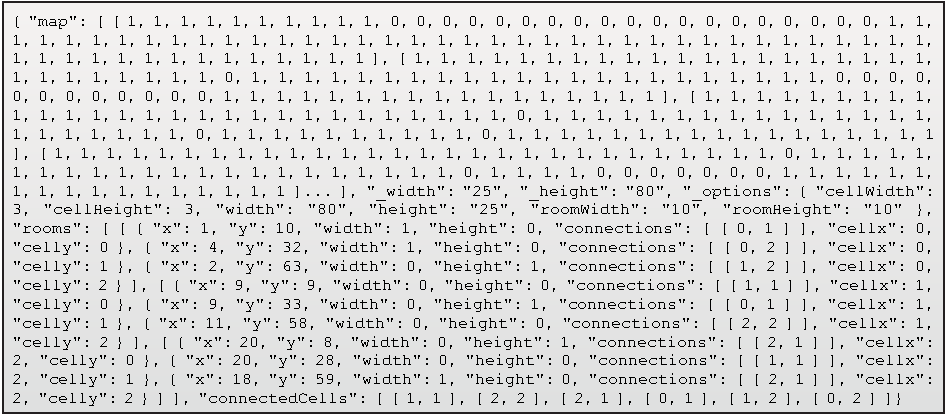
\includegraphics[width=0.90\textwidth]{obrazky/dunglib_mattmcfarland.pdf}
    \caption{Ukázka JSON odpovědi webového serveru  \href{https://github.com/MattMcFarland/rot-web-api}{Rot Web API (MattMcFarland)} na HTTP GET požadavek pro generátor \texttt{Rogue}. Část \texttt{map} obsahuje 2D matici dlaždic (zkráceno), následné části s~podtržítky obsahují obecnou charakteristiku dungeonu a další části představují obecný popis místností a propojení mezi nimi.}
    \label{img:dunglib_mattmcfarland}
\end{figure}
\par
Tento projekt ukazuje zajímavý koncept generátoru herních úrovní v~podobě webové služby.
Jednoduchým voláním HTTP GET požadavků s~příslušnými parametry lze vygenerovat požadovaný výstup.
Server dokáže obsloužit spoustu klientů pomocí vygenerovaných dat nezávisle na programovacím jazyce, který používají.
Nevýhodou je, že je potřeba server, na kterém bude služba trvale běžet.
Dostupné algoritmy, jejich parametry a výstupy jsou navíc poměrně triviální.

%--------------------------------------------------------------

\subsection{Shrnutí existujících řešení}

%--------------------------------------------------------------

Knihovny představené v~části \ref{sec:dostupne_knihovny} mají výhody i nevýhody, z~nichž se lze při vývoji této knihovny poučit.
Důležitou otázkou je \textbf{použitelnost knihovny} z~hlediska programovacího jazyku nebo platformy.
Ideální by bylo, kdyby byla knihovna použitelná univerzálně, například jako služba, která obslouží požadavky klientů, případně jako program spustitelný z~libovolného systému či jazyku.
Dalším důležitým faktorem je \textbf{uživatelská přívětivost}.
Uživatel by měl mít k~dispozici jasně definované rozhraní pro definování parametrů, které ovlivní výstup, bez nutnosti tyto parametry složitě nastavovat přímo v~kódu knihovny.
Neméně důležitý je pak \textbf{formát výstupu}.
Důležitá není pouze podpora různých souborových formátů, ale i přizpůsobení výstupu podle toho, pro jaké případy užití bude výstup navržen.
Například pokud bude uživatel chtít výstup vykreslit na rovinu, mřížka buněk je daleko vhodnější alternativou, než složité grafové struktury sestávající se z~uzlů a hran.

%--------------------------------------------------------------

\chapter{Návrh knihovny pro generování dungeonů}
\label{ch:navrh} % 4

%--------------------------------------------------------------

Hlavním cílem této bakalářské práce je tvorba knihovny pro procedurální generování dungeonů.
Před vytvořením samotné knihovny je vhodné tuto knihovnu obecně navrhnout -- jaké jsou na ni kladeny požadavky, co musí knihovna dělat, jak ji bude uživatel používat a jaká tedy bude její celková podoba.
O~tom pojednává tato kapitola.
V~kapitole \ref{ch:implementace} pak bude knihovna podle návrhu implementována.

%--------------------------------------------------------------

\section{Požadavky na knihovnu}

%--------------------------------------------------------------

Před vytvořením samotného návrhu je potřeba si uvědomit, jak bude knihovna používána a jaké vlastnosti tedy musí splňovat.
Knihovna je určena především pro vývojáře, kteří nechtějí herní úrovně vytvářet ručně a hledají jednoduchý způsob, jak je generovat procedurálně.
Knihovna by jim tedy měla ušetřit čas, ale přitom vytvářet úrovně, které budou moci použít ve svých hrách.
Vývojář knihovnu jednoduše zahrne do svého projektu a prostřednictvím jejího rozhraní určí požadované parametry.
Pokud vývojář pracuje v~jiném jazyce, měl by být schopen knihovnu i přesto využít.
Po spuštění generátoru dojde k~vytvoření struktury herní úrovně, která bude respektovat požadavky vývojáře.

%--------------------------------------------------------------

\subsection{Funkce knihovny}

%--------------------------------------------------------------

Knihovna musí uživateli umožnit vytvořit a vložit vstupní konfiguraci, tuto konfiguraci validovat a případně uživatele informovat o~chybách, aby mohl konfiguraci opravit.
Poté se tento vstup předá generátoru, který podle konfigurace vygeneruje herní úroveň.
Pokud by došlo během generování k~chybám, uživatel musí být o~této skutečnosti informován.
Následně musí být uživateli nabídnuty různé způsoby, jakými může k~výsledné výstupní struktuře přistupovat a zpracovat ji.

%--------------------------------------------------------------

\subsection{Cílové vlastnosti}
\label{ssec:cilove_vlastnosti}

%--------------------------------------------------------------

Při vývoji knihovny bude nutné brát zřetel na tyto vlastnosti:
\begin{itemize}
    \item \textit{Rychlost:} Knihovna by měla dosáhnout výsledku v~rozumném čase, není jisté, kdy vývojář generátor spustí.
    Může to být na \uv{načítací obrazovce}, nebo dynamicky přímo ve hře.
    Knihovna by neměla vývojáře nutit k~tomu, aby herní úrovně postupně generoval na samostatném vláknu, proto je rychlost klíčová, aby se hra \uv{nezasekla} a hráč nemusel čekat.
    \item \textit{Přizpůsobitelnost:} Knihovna by měla nabízet takové parametry pro přizpůsobení výstupu, aby pokryla co největší množství použití.
    Samozřejmě nelze podchytit všechny případy užití, vzorem ale může být analýza existujících her.
    Knihovna by vývojáři zároveň měla umožnit, aby si vygenerovaný výstup mohl dále přizpůsobovat o~prvky, které knihovna nepodporuje.
    Například doplnit do vygenerované obdélníkové místnosti sloupořadí.
    \item \textit{Jednoduchost:} Knihovna musí ušetřit vývojářům čas.
    Její použití by proto mělo být jednoduché a intuitivní.
    \item \textit{Spolehlivost:} Aby mohl vývojář knihovnu ve své hře použít, musí se spolehnout na její výstup.
    U~prvků herní úrovně, které vývojář označí jako povinné, musí knihovna \textbf{zajistit}, že se budou ve vygenerovaném výstupu skutečně nacházet.
    Pokud bude vývojář například generovat úroveň, která bude obsahovat místnost s~hlavním nepřítelem, nemůže dojít k~tomu, že by ve výsledné úrovni chyběla.
    \item \textit{Různorodost:} Vývojář knihovnu použije, protože chce, aby byly herní úrovně náhodně generované.
    S~tím totiž úzce souvisí to, za jak dlouho je hráč začne vnímat jako repetitivní a stereotypní.
    Knihovna proto musí zajistit, že hráč pokaždé prožije jedinečný zážitek.
    \item \textit{Opakovatelnost:} Knihovna by měla obsahovat mechanismus, který umožní při zadání stejných parametrů opakovaně získat tentýž výstup (je-li to vyžadováno vývojářem).
    Může se jednat například o~klíč, který se použije jako semínko generátoru náhodných čísel.
    \item \textit{Univerzálnost:} Knihovna, a především její výstup, by měly být univerzálně použitelné (do té míry, jak je to technicky možné a proveditelné). 
\end{itemize}
Knihovna bude z~hlediska těchto vlastností testována v~kapitole \ref{ch:testovani}.

%--------------------------------------------------------------

\subsection{Struktura a vlastnosti dungeonu}

%--------------------------------------------------------------

Herní úroveň generovaná touto knihovnou by měla obsahovat místnosti specifikované uživatelem a tyto místnosti musí být vzájemně vhodným způsobem propojeny na rovině.
Každá místnost může být propojena s~více místnostmi (ideálně nejbližšími), místnosti mohou tvořit smyčky ale i \uv{slepé konce}.
Je nutné nalézt ideální poměr mezi \uv{propojeností} místností a linearitou.
Místnosti se nesmí vzájemně překrývat, ale zároveň by dungeon neměl obsahovat místnosti příliš vzdálené od ostatních místností.
Herní úroveň nesmí obsahovat žádné osamostatněné místnosti, tzn. hráč by měl být vždy schopen dostat se z~jednoho konce herní úrovně na druhý.
V~případě, že jsou místnosti od sebe vzdáleny, lze je propojit chodbou.
Chodba by však neměla být příliš dlouhá, měla by respektovat velikosti místností a celkové herní úrovně.
Pokud na sebe místnosti doléhají, chodba není třeba.
Vývojář však musí být informován o~tom, zda mají být dvě sousední místností propojeny či nikoliv.
\par
Hry obsahující dungeony jsou velice často s~isometrickou grafikou a jednotlivé grafické assety\footnote{\textbf{Grafický asset} -- vizuální reprezentace objektu použitého ve hře, typicky se jedná například o~3D model s~texturou nebo rastrový obrázek} herních úrovní reprezentují nějakou jejich diskrétní část (například asset znázorňující blok stěny).
Proto je vhodné, aby byl dungeon rozčleněn do dlaždic a každý prvek dungeonu bude tvořen jednou nebo více dlaždicemi.
Díky tomu bude moci vývojář dlaždicím přiřadit konkrétní grafickou podobu.

%--------------------------------------------------------------

\subsection{Způsoby použití knihovny}

%--------------------------------------------------------------

Knihovna musí nějakým způsobem převzít konfiguraci, tu zpracovat a předat na výstup výslednou strukturu.
Aby byla co nejpoužitelnější, je vhodné, aby ji šlo používat různými způsoby, z~nichž minimálně jeden nesmí být závislý na použitém jazyce.
Existují různé způsoby, jakými se knihovny používají:
\begin{itemize}
  \item{Knihovna jako součást projektu. Standardní vložení knihovny do projektu a volání funkcí či metod jejího veřejného rozhraní, knihovna, nebo minimálně její volané části, jsou poté většinou součástí samotného projektu (nejsou-li již dostupné v~prostředí, kde je projekt spouštěn). Taková knihovna může mít podobu binárního souboru (nutné další zpracování programem zvaným \textit{linker}) nebo skriptu. Tento způsob redukuje možnost využití na jeden konkrétní programovací jazyk. K~dispozici však mohou být specializované nástroje, které dokážou knihovnu transformovat pro využití v~jiných jazycích. Příkladem může být projekt SWIG\footnote{\url{http://www.swig.org}}, který umožňuje propojit programy napsané v~jazyce C a C++ s~vyššími programovacími jazyky.}
  \item{Knihovna jako webová služba. Knihovna je spuštěna na webovém serveru a zpracovává příchozí požadavky klientů, které ji webový server předá. V~současnosti se nejčastěji používá architektura rozhraní REST, která definuje komunikační protokol pro komunikaci mezi aplikacemi a klienty prostřednictvím HTTP volání.}
  \item{Knihovna jako program. Knihovna přijímá přímý nebo souborový vstup a vytváří výstup. Knihovnu lze tudíž spouštět jako kterýkoliv jiný program. S~využitím funkcí operačního systému lze pak knihovnu spouštět jiným programem napsaným v~libovolném jazyce.}
\end{itemize}
Konkrétní způsoby, jakými se bude používat tato knihovna, budou záviset na implementačním jazyce.

%--------------------------------------------------------------

\section{Struktura knihovny a popis komponent}

%--------------------------------------------------------------

Obecný návrh struktury knihovny se stručným popisem je uveden na obrázku \ref{img:lib_design}.
\begin{figure}[hbt]
    \centering
    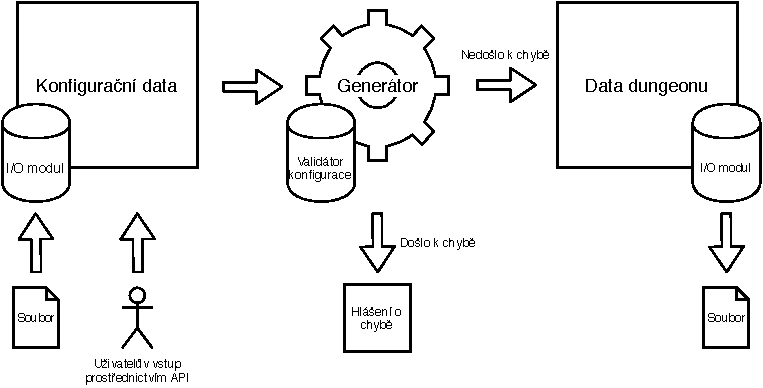
\includegraphics[width=1.0\textwidth]{obrazky/navrh_knihovny.pdf}
    \caption{Obecný návrh struktury knihovny -- knihovna načte konfigurační data (ať už zadaná uživatelem prostřednictvím API nebo jako soubor), tato data poté předá generátoru, který konfiguraci prověří a vygeneruje dungeon, který lze poté také převést do souborové podoby.}
    \label{img:lib_design}
\end{figure}
Tato část obsahuje popis jednotlivých komponent knihovny.
Podrobnější popis navrhovaného algoritmu generátoru se nachází v~části \ref{sec:navrh_algoritmu}.

%--------------------------------------------------------------

\subsection{Vstupní konfigurace}

%--------------------------------------------------------------

Vstupní konfigurace je důležitý prvek, který generátoru říká, jakým způsobem má pracovat.
Tuto konfiguraci bude moci uživatel určit pomocí přiloženého rozhraní, případně pomocí konfiguračního souboru.
Konfigurace bude obsahovat informace o~tvarech a počtech požadovaných místností a globální parametry.

\subsubsection{Tvary místností a tvarové šablony}
Každá místnost musí mít přiřazen tvar.
Ty se budou definovat zvlášť.
Tvary místností budou mít svůj jedinečný název (identifikátor), který lze poté používat v~definicích místností.
Každý tvar tedy půjde využít ve více místnostech.
Tvar jednoznačně definuje, jak bude daná místnost velká a který prostor bude zaujímat.
Uživatel bude moci tvar definovat dvěma způsoby:
\begin{enumerate}
    \item Exaktním ručním zápisem se znaky reprezentujícími jednotlivé dlaždice, kdy každý z~nich představuje prostor místnosti nebo prázdný prostor
    \item Použitím předem připravené šablony s~parametry, například šablona pro generování obdélníků s~šířkou a výškou ze zadaného rozsahu, kdy generátor při každém vygenerování místnosti vytvoří různě veliký obdélníkový tvar
\end{enumerate}

\subsubsection{Místnosti}
Uživatel musí definovat, které místnosti v~dungeonu chce.
Každá místnost bude mít svůj jedinečný název (identifikátor) a přiřazený tvar.
Uživatel bude moci určit, kolik daných místností se má v~dungeonu vygenerovat (lze zapsat i jako číselný rozsah od-do).
U~každé místnosti bude moci uživatel určit, zda ji může generátor náhodně otáčet (v~krocích o~velikosti 90$^{\circ}$).

\subsubsection{Globální parametry}
Kromě místností a jejich tvarů bude moci uživatel určit některá obecná nastavení.
Jedním z~nich je například \textit{semínko} (číselné nebo textové), které uživateli umožní vygenerovat tentýž dungeon opakovaně.
Pokud uživatel semínko vynechá, použije se náhodné.
Dalším parametrem bude explicitní určení \textit{formátu výstupního souboru}, který použije I/O modul v~případě, že se má výstup uložit do souboru.
Při vynechání se použije stejný formát, který byl použit ve vstupním souboru s~konfigurací.

%--------------------------------------------------------------

\subsection{Výstupní data dungeonu}

Hlavním důvodem, proč knihovnu uživatel využije, je získání dat reprezentujících dungeon.
Aby tato data mohl uživatel využít, je důležité, aby na ně knihovna nabízela více pohledů, z~nichž si uživatel vybere pro něj nejvhodnější.
Cílem je uživateli co nejvíce usnadnit využití výstupních dat.

\subsubsection{Graf místností}
Dungeony nejsou nic víc, než kolekce místností propojené chodbami.
Uživatel tedy musí vědět, které místnosti dungeon obsahuje a jak jsou propojeny.
Výstupní data proto budou obsahovat seznam místností, které vyplývají ze vstupní konfigurace.
Každá místnost bude obsahovat vygenerovaný jedinečný číselný \textit{identifikátor}, který představuje identifikátor uzlu v~pomyslném grafu.
Dále bude u~místností uveden \textit{název} místnosti tak, jak jej uvedl uživatel ve vstupní konfiguraci (aby uživatel věděl, o~jakou místnost jde, když jich je více různých).
Každá místnost musí mít \textit{tvar}, ten bude ve výstupních datech reprezentován maticí znaků reprezentujících prázdnou, resp. vyplněnou buňku.
Tvar může vycházet z~tvaru zadaného uživatelem nebo se může jednat o~tvar vygenerovaný knihovnou v~případě, že ve vstupní konfiguraci byl tvar místnosti definován šablonou.
U~místností nemůže chybět ani \textit{pozice} v~rámci dungeonu.
Souřadnice místnosti jsou vždy kladné a určují pozici buňky, která je ve tvaru místnosti doplněném na obdélník v~levém horním rohu.
A~konečně -- u~každé místnosti bude \textit{seznam propojení} -- tedy seznam místností, se kterými je místnost přímo propojena chodbou.
Místnosti v~tomto seznamu budou reprezentovány svými číselnými identifikátory, takže uživateli stačí vyhledat si je v~seznamu místností.
Díky tomu má uživatel veškeré informace potřebné pro sestavení grafu místností.

\subsubsection{Chodby}
Výstupní data budou obsahovat také seznam chodeb.
Chodby budou ve výstupních datech reprezentovány jako speciální místnosti.
U~každé bude uveden její \textit{číselný identifikátor}, \textit{tvar} reprezentovaný maticí znaků, \textit{pozice} v~dungeonu a \textit{místnosti, které propojuje}.

\subsubsection{Mřížka buněk}
Pro snadnější použití výstupních dat budou do výstupních dat účelově zanesena redundantní data v~podobě mřížky buněk, která bude umožňovat například sekvenční zpracování v~cyklu.
Každá buňka bude obsahovat \textit{pozici} v~dungeonu, její \textit{typ} (např. stěna, místnost, chodba, prázdný prostor atd.) a případně \textit{identifikátor} příslušné místností nebo chodby, ke které náleží.

\subsubsection{Další data}
Ve výstupní konfiguraci bude uvedeno i \textit{semínko}, podle kterého byl dungeon vygenerován.
To je užitečné v~případě, kdy uživatel semínko do konfigurace nezadal, a tudíž bylo vybráno náhodně.

%--------------------------------------------------------------

\subsection{I/O modul}

%--------------------------------------------------------------

Knihovna bude podporovat také souborový vstup a výstup.
Uživatel bude moci načíst soubor obsahující vstupní konfiguraci.
Soubor se zpracuje a vytvoří se z~něj konfigurační struktura stejná, kterou by uživatel mohl vytvořit sám ručně prostřednictvím rozhraní knihovny.
Konfigurační struktura se pak předá generátoru jako obvykle.
\par
Do souboru bude možné uložit i dungeon samotný, což je důležité zejména pro použití knihovny nezávisle na programovacím jazyku.
K~tomuto účelu bude možné knihovnu spouštět jako program, kdy po spuštění bude knihovna očekávat cestu ke konfiguračnímu souboru na standardním vstupu.
Na základě přípony tohoto souboru se obsah souboru zpracuje odpovídajícím způsobem.
Budou se přitom kontrolovat veškeré náležitosti a syntaktická správnost souborového formátu.
V~případě chyby v~konfiguraci, syntaktické chyby nebo chyby generátoru bude uživatel informován tím, že se místo výstupu vytvoří soubor s~názvem \texttt{err-XX.err}, kde \texttt{XX} bude nahrazeno časovým razítkem spuštění generátoru.
Pokud bude generování úspěšné, vytvoří se soubor s~názvem \texttt{dungeon-XX.YY}, kde \texttt{XX} bude nahrazeno časovým razítkem spuštění generátoru a \texttt{YY} bude představovat příponu výstupního souboru, která bude určena podle přípony vstupního konfiguračního souboru nebo explicitním určením přípony uživatelem v~konfiguraci.
\par
Pro větší použitelnost by měla knihovna podporovat pokud možno více než jeden formát používaný pro přímou výměnu dat.
Mělo by se jednat ideálně o~snadno lidsky čitelné formáty, které lze programově zpracovat, umožňují zápis kolekcí (například v~podobě seznamů) a nabízejí širokou podporu napříč programovacími jazyky, aby bylo možné výsledný dungeon zpracovat bez nutnosti ručního zpracovávání dat.
Podle článku na blogu Nordic APIs, skandinávského pořadatele událostí pro uživatele a nadšence rozhraní API, jsou nejpoužívanějšími formáty pro přímou výměnu dat formáty XML, JSON a YAML\cite{lit:file_formats}.
I/O modul knihovny by tak měl podporovat alespoň tyto tři.

%--------------------------------------------------------------

\subsection{Generátor}

%--------------------------------------------------------------

Generátor je nejdůležitější komponentou celé knihovny.
V~knihovně se bude skládat ze dvou částí -- validátoru konfigurace, který se ujistí, že konfigurace obsahuje informace, které jsou ke generování potřeba, a samotný generovací modul, který podle vstupu vygeneruje výslednou strukturu, případně oznámí chybu.
Generátor bude obsahovat několik dílčích modulů, které budou mít na starost jednotlivé kroky algoritmu popsaného v~části \ref{sec:navrh_algoritmu}.
Navržený generátor musí splňovat veškeré cílové vlastnosti stanovené v~části \ref{ssec:cilove_vlastnosti}, což bude ověřeno v~kapitole \ref{ch:testovani}.

%--------------------------------------------------------------

\section{Návrh algoritmu generátoru}
\label{sec:navrh_algoritmu}

%--------------------------------------------------------------

Algoritmus generátoru, pomocí kterého dojde ke generování výsledné struktury dungeonu podle vstupní konfigurace, bude rozdělen do série kroků, z~nichž v~každém bude provedena funkčně a logicky oddělená činnost, které jsou však vzájemně závislé.
Pokud dojde v~kterémkoliv kroku k~chybě, generování nemůže dále pokračovat.
Krok by mělo být možné opakovat pro případ, kdy jsou k~jeho úspěšnému provedení potřeba příznivé vstupně-výstupní podmínky (typicky situace, ve kterých hraje roli náhodný generátor čísel).
\par
Algoritmus se bude podobat algoritmu představenému v~části \ref{ssec:dungeongenerator_jongallant}, protože vyhovuje požadavkům knihovny, ačkoliv některé jeho kroky budou přidány, pozměněny nebo úplně vynechány.
\par
Veškeré funkce využívající náhodných jevů budou využívat společný generátor, který bude vytvořen podle stanoveného semínka.
Taktéž budou využívány takové kolekce a struktury, které umožňují iterovat prvky v~předvídatelném pořadí.
Díky tomu bude moci být uživateli nabídnuta možnost vygenerovat tentýž dungeon opakovaně s~totožným výsledkem.

%--------------------------------------------------------------

\subsection{Vkládání místností}

%--------------------------------------------------------------

Celý algoritmus začne vkládáním místností do dungeonu.
Nejdříve se načtou požadované místnosti v~konfiguraci a vkládací modul je projde jednu za druhou.
U~každé předepsané místnosti bude načten jejich počet a pokud se jedná o~rozsah, vybere se náhodný počet z~tohoto rozsahu (s~rovnoměrným rozdělením pravděpodobnosti).
Následně se místnostem přidělí tvar -- buď z~konfigurace, nebo se náhodně vygeneruje ze šablony.
V~případě, že je povolena rotace tvaru, dojde k~náhodné rotaci o~0, 90, 180 nebo 270 stupňů.
Nakonec budou místnosti umístěny tak, že jejich střed bude ležet na počátku souřadnic dungeonu (bod [0,0]) s~mírnou odchylkou.
\begin{figure}[hbt]
    \centering
    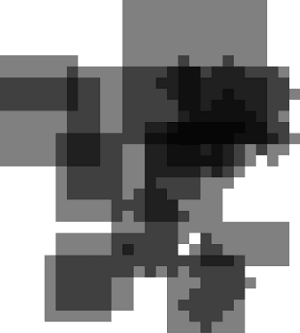
\includegraphics[width=0.4\textwidth]{obrazky/navrh1.png}
    \caption{Znázornění podoby dungeonu po vložení místností -- místnosti se nacházejí v~oblasti kolem středu s~mírnou odchylkou. Překrytí je znázorněno tmavší šedou barvou.}
    \label{img:navrh1}
\end{figure}

%--------------------------------------------------------------

\subsection{Rozprostření místností}

%--------------------------------------------------------------

Po vložení místností bude nutné místnosti rozložit po ploše tak, aby se žádná místnost nepřekrývala.
Pro jednodušší kontrolu překrývání bude algoritmus doplňovat tvary místností na obdélník.
\par
Kontrola, zda se dva obdélníky překrývají, je pak jednoduchá.
Stačí zkontrolovat, zda je jeden obdélník vlevo od druhého, resp. zda je jeden obdélník pod druhým obdélníkem.
Toho lze docílit kontrolou, zda je levá hrana prvního obdélníku více vpravo než pravá hrana druhého obdélníku a naopak, resp. zda je horní hrana prvního obdélníku více dole než dolní hrana druhého obdélníku.
\par
Relativně náročnějším pak je algoritmus pro rozprostření obdélníků po herní ploše.
Při implementaci lze vycházet z~techniky Separating Axis Theorem (SAT), která říká, že pokud existuje osa, která se neprotíná s~projekcemi obou objektů, tyto objekty se nepřekrývají\cite{lit:sep_axis_theorem}.
Součástí této techniky je vyhledávání mezery mezi objekty pomocí projekce objektů na obecnou osu.
V~tomto případě jsou obdélníky vždy rovnoběžné s~osami souřadnic, a tudíž je situace výrazně jednodušší.
Zjednodušeně řečeno stačí vyhledat takový vektor, o~který je nutné jeden obdélník po určité ose posunout, aby se přestal překrývat s~druhým obdélníkem.
Lze přitom otestovat vodorovnou i svislou osu a vybrat nejmenší možný vektor, buď na jedné ose, nebo na obou současně.
Tento vektor se poté přičte k~souřadnicím obdélníku.
Další možnou variantou je určit náhodný úhel, po kterém bude obdélník posouván, a poté vypočítat vektor, o~který je nutné obdélník pod daným úhlem posunout, aby se přestal překrývat s~jiným obdélníkem.
Vzhledem k~faktu, že souřadnice v~dungeonu neobsahují desetinná místa, nebude tento úhel dodržován úplně přesně.
\par
Důležitým faktorem je pak i způsob iterování mezi obdélníky.
Jednou možnou variantou je sériové iterování obdélníků v~náhodném pořadí a následné testování kolizí se všemi ostatními obdélníky.
Při každé kontrole se získá vektor, o~který je nutné první obdélník posunout po ose, aby nekolidoval s~druhým.
Pokud je velikost tohoto vektoru větší než velikost aktuálně uloženého vektoru, vektor se uloží.
Nakonec se obdélník o~největší vektor posune a jeho pozice se uzamkne.
Takto budou iterovány všechny obdélníky, dokud se nebude žádný překrývat.
Druhou možnou variantou je iterování obdélníků v~náhodném pořadí, přičemž pro každý z~nich se na začátku určí úhel, ve kterém se bude posouvat.
Postupným posunováním obdélníku pod tímto úhlem a kontrolováním kolizí budou všechny obdélníky rozprostřeny.
Aby však obdélníky lépe \uv{zapadly} do mezer mezi paprsky tvořenými z~již rozprostřených obdélníků, je vhodné k~úhlu přičíst nebo odečíst náhodnou odchylku.
\par
Ze všech zmiňovaných metod bude vybrána ta, která bude mít prostorově nejpřijatelnější výsledky a dosáhne klidového stavu v~nejkratším čase.
Číselné parametry, úhly a odchylky pro algoritmy se určí experimentálně.
\begin{figure}[hbt]
    \centering
    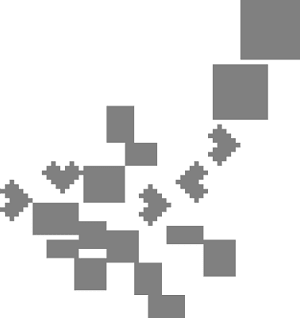
\includegraphics[width=0.4\textwidth]{obrazky/navrh2.png}
    \caption{Znázornění podoby dungeonu po rozprostření místností -- místnosti se nikde nepřekrývají a mohou být mezi nimi menší mezery.}
    \label{img:navrh2}
\end{figure}

%--------------------------------------------------------------

\subsection{Tvorba grafu}

%--------------------------------------------------------------

Dalším krokem je propojení místností.
Cílem je, aby byla každá místnost propojena alespoň s~jednou další místností a aby bylo vždy možné najít cestu z~jedné místnosti do kterékoliv jiné.
K~tomuto účelu bude vytvořena množina bodů grafu ze středů místností.
Tyto středy budou následně propojeny trojúhelníky metodou Delaunayovy triangulace, která vychází z~podmínky, že uvnitř kružnice opsané libovolnému trojúhelníku se nebude nacházet žádný vrchol jiného trojúhelníku.
Následně bude vyhledána minimální kostra grafu, přičemž hrany budou ohodnoceny podle vzdálenosti mezi místnostmi podle Pythagorovy věty (s~vynechanou odmocninou pro vyšší výpočetní rychlost).
Vzniklá kostra neobsahuje žádné smyčky, což je pro dungeon nezvyklé.
Proto budou smyčky do dungeonu zaneseny.
Algoritmus se přitom zaměří na vrcholy prvního stupně (tedy místnosti, které jsou propojeny právě s~jednou další místností).
Tyto místnosti budou s~určitou pravděpodobností opět propojeny s~jedním ze svých původních sousedů.
Důležitá je však vzdálenost mezi těmito místnostmi -- Delaunayova triangulace má tendenci vytvářet dlouhé hrany na okrajích grafu, což by způsobilo generování příliš dlouhých chodeb, proto se bude při propojování zohledňovat i vzdálenost -- pokud bude mnohem větší než je průměrná vzdálenost mezi místnostmi v~dungeonu, k~propojení nedojde.

\begin{figure}[hbt]
    \centering
    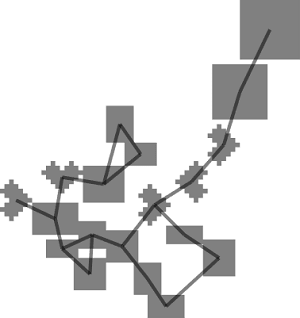
\includegraphics[width=0.4\textwidth]{obrazky/navrh3.png}
    \caption{Znázornění podoby dungeonu po propojení místností -- hrany grafu jsou znázorněny šedými čárami. Graf obsahuje tři smyčky, které byly vytvořeny uměle z~minimální kostry.}
    \label{img:navrh3}
\end{figure}

%--------------------------------------------------------------

\subsection{Propojování chodbami}

%--------------------------------------------------------------

Místnosti, které jsou propojené v~grafu, je nutné propojit i fyzicky v~dungeonu chodbami.
Mohou nastat dvě situace:
\begin{enumerate}
    \item Místnosti mají společnou část vodorovné nebo svislé hrany (společné souřadnice X nebo Y v~určitém rozsahu) -- pokud se místnosti nedotýkají, stačí je propojit rovnou chodbou.
    \item Místnosti nejsou pod sebou ani vedle sebe -- tyto místnosti se propojí chodbou ve tvaru písmene L, přičemž začátek a konec chodby bude začínat u~rohů místností tak, aby nemohlo dojít ke kolizi s~jinou místností nebo chodbou. Chodba pak bude mít nejmenší možnou délku a obsah jejího tvaru doplněný na obdélník bude co nejmenší.
\end{enumerate}
V~některých případech však ke kolizím dojít může -- například při křížení přímých chodeb propojujících dvě a dvě místností.
V~takových případech lze tento problém vyřešit několika způsoby:
\begin{enumerate}
    \item Sloučením chodeb, kdy výsledná chodba bude propojovat všechny místnosti současně.
    \item Implementací algoritmu pro hledání cesty, výsledná chodba by pak byla několikanásobně lomená čára.
    \item Odstraněním propojení mezi místnostmi způsobujících kolizi, případně přepojením těchto místností k~jiným místnostem vhodným způsobem.
    \item Zahozením dungeonu a vygenerováním nového.
\end{enumerate}
Protože tato knihovna neumožňuje určování pořadí místností za sebou a omezování místností, se kterými jsou propojeny, lze použít variantu číslo 1.
Pokud by však v~budoucnu došlo k~implementaci těchto konfiguračních možností, musel by se problém křížících chodeb řešit alternativním způsobem.
\begin{figure}[hbt]
    \centering
    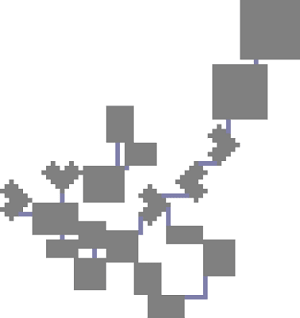
\includegraphics[width=0.4\textwidth]{obrazky/navrh4.png}
    \caption{Znázornění podoby dungeonu po propojení místností chodbami -- pokud se místnosti dotýkají, chodba není potřeba. Na obrázku lze pozorovat i chodbu ve tvaru písmene L.}
    \label{img:navrh4}
\end{figure}

%--------------------------------------------------------------

\subsection{Normalizace souřadnic}

%--------------------------------------------------------------

Nakonec budou upraveny veškeré souřadnice tak, aby nebyly záporné.
Jednoduše se projdou veškeré souřadnice objektů na ose X a na ose Y a uloží se nejvíce záporné hodnoty pro každou z~těchto os.
Jejich absolutní hodnoty se poté přičtou ke všem souřadnicím všech objektů v~dungeonu, čímž dojde k~posunutí objektů na rovině dungeonu vpravo dolů.
Výsledné souřadnice budou vždy kladné.

%--------------------------------------------------------------

\chapter{Implementace navržené knihovny}
\label{ch:implementace} % 5

%--------------------------------------------------------------

Tato kapitola obsahuje popis implementačních detailů, zejména použité technologie, strukturu knihovny a informace o~implementaci jednotlivých částí.
V~kapitole již nejsou uváděny teoretické detaily o~tom, jak samotné generování funguje.
To je vysvětleno zejména v~kapitole \ref{ch:navrh}.

%--------------------------------------------------------------

\section{Použité technologie}

%--------------------------------------------------------------

Knihovna byla vyvinuta v~programovacím jazyce \textbf{Java} verze 8 SE.
Java je široce využívaným programovacím jazykem s~rozsáhlou podporou objektových paradigmat, pomocných funkcí a knihoven.
Dalšími vhodnými alternativami by byl například jazyk C\#, který se široce používá ve vývojářském systému Unity, nebo jazyk C++.
Protože je však knihovna koncipována tak, aby byla použitelná z~kteréhokoliv jazyka, Java je spíše volba plynoucí z~osobní preference.
\par
Pro automatizované sestavování projektu a správu závislostí byl využit systém Apache Maven\footnote{\url{https://maven.apache.org}}, který na základě obsahu souboru \texttt{pom.xml} v~kořenovém adresáři dokáže při sestavování automaticky stáhnout a připojit veškeré závislosti a pomocí příslušných pluginů také vytvořit spustitelný balík JAR obsahující veškeré závislosti.
\par
Projekt využívá také množství knihoven.
Za zmínku stojí knihovny projektu Apache Commons\footnote{\url{https://commons.apache.org}} s~užitečnými funkcemi pro práci s~řetězci, čísly a soubory, knihovna pro Delaunayovu triangulaci\footnote{\url{https://www.cs.bgu.ac.il/~benmoshe/DT/Delaunay\%20Triangulation\%20in\%20Java.htm}} z~izraelské Ben Gurionova univerzity v~Negevu, knihovna JGraphT\footnote{\url{https://jgrapht.org}} pro práci z~grafy, ze které knihovna využívá algoritmus pro hledání minimální kostry grafu, a knihovna Jackson\footnote{\url{https://github.com/FasterXML/jackson}} pro práci se soubory ve formátu XML a její doplňkové moduly pro práci s~formáty JSON a YAML.

%--------------------------------------------------------------

\section{Struktura knihovny}

%--------------------------------------------------------------

Projekt je rozčleněn do balíků podle jejich účelu, v~seznamu je uvedena vždy pouze významová část názvu (bez společné části \texttt{cz.iwitrag.procdungen}).

\begin{itemize}
    \item cz.iwitrag.procdungen -- předpona všech ostatních balíků (dále bude vynechávána). Obsahuje třídu \texttt{Main}, která se spouští při spuštění balíku JAR knihovny.
    \item api -- obsahuje vše, s~čím přijde do kontaktu uživatel při práci s~knihovnou. Důležitá je třída \texttt{ProcDunGenApi}, která je výchozím bodem pro předání vytvořené konfigurace a spuštění generátoru.
    \item api.configuration -- třídy pro ruční (bez souboru) nastavení konfigurace generátoru.
    \item api.configuration.files -- I/O modul konfigurace pro vytvoření konfigurace ze souboru, skládá se zejména z~POJO\footnote{\textbf{POJO} -- Plain old Java object, obyčejný Java objekt bez jakýchkoliv restrikcí ze strany návrhových vzorů, konvencí nebo frameworků} tříd, které se v~tomto případě používají k~uchovávaní dat načtených ze souboru před jejich zpracováním.
    \item api.data -- třídy obsahující data vytvořeného dungeonu určené pro zpracování uživatelem.
    \item api.data.files -- I/O modul dat s~dungeonem pro jejich uložení do souboru.
    \item generator -- obsahuje vše související se samotným generátorem.
    \item generator.implementations.physical -- implementace jediného generátoru knihovny, obsahuje třídy pro zpracování jednotlivých fází generování.
    \item generator.templates -- třídy pro generování tvarů místností podle šablon.
    \item util -- pomocné třídy pro práci s~tvary a čísly.
\end{itemize}

%--------------------------------------------------------------

\section{Konfigurační API}

%--------------------------------------------------------------

Pro vytvoření konfigurace předávané generátoru obsahuje knihovna třídy, které uživatel jednoduše naplní požadovanými údaji.
Nejdůležitější je třída \texttt{DungeonConfiguration}, která sdružuje veškeré konfigurační náležitosti v~sobě: tvary místností, místnosti samotné, požadovaný typ výstupního souboru (nepovinné) a explicitně zadané semínko (nepovinné).
Kromě metod pro nastavování výše uvedeného obsahuje tato třída statickou metodu \texttt{fromFile()} pro vytvoření instance konfigurace ze souboru a metodu \texttt{validate()} pro ověření správnosti konfigurace.
Tuto metodu knihovna volá před spuštěním generátoru automaticky.
\par
Třída \texttt{RoomShape} představuje tvar místnosti.
Tvar lze určit přímo jako matici znaků (pomocí třídy \texttt{TextualShape}) nebo pomocí šablony (třída \texttt{RoomTemplate}).
V~případě, že chce uživatel použít předem připravenou šablonu, musí zjistit její název (například z~dokumentace) a parametry, které přijímá.
Pokud budou tyto údaje chybět nebo budou neúplné či nesprávně zadané, uživatel bude informován.
\par
Místnosti lze definovat pomocí třídy \texttt{Room}.
Každá místnost má určitý název a tvar a dále musí mít uveden počet.
Ten se uvádí jako \texttt{IntRange}, tedy celočíselný rozsah.
Generátor poté vybere hodnotu z~rozsahu, což zvyšuje variabilitu.
U~každé místnosti lze i nastavit, zda může generátor tvar náhodně otáčet.

%--------------------------------------------------------------

\section{Zapouzdření výstupních dat}

%--------------------------------------------------------------

Výstupní data dungeonu jsou zapouzdřena ve třídě \texttt{Dungeon}, která obsahuje vygenerované místnosti (třída \texttt{Room}) a chodby (třída \texttt{Corridor}), mřížku buněk tvořících dungeon (třída \texttt{Grid}) a použité semínko (definované uživatelem nebo náhodně vybrané).
Třída dále obsahuje metody \texttt{toYaml()}, \texttt{toJson()} a \texttt{toXml()}, které zapisují výstupní data do souboru v~příslušném formátu.
\par
Mřížka získaná voláním metody \texttt{getGrid()} se generuje, jakmile je potřeba, a je poté uložena.
V~případě, že by došlo k~úpravě dungeonu (např. smazání místnosti), uložená mřížka se smaže, protože je neaktuální.
Mřížka vzniká tak, že se v~cyklu procházejí jednotlivé místnosti a chodby, získá se jejich pozice (levý horní roh tvaru doplněného na obdélník) a poté se v~cyklu propisují buňky jejich tvaru do mřížky s~relativními pozicemi.
Mřížka je tvořena buňkami reprezentovanými třídou \texttt{GridCell}.
Každá buňka obsahuje pozici v~rámci mřížky, typ a případnou referenci na příslušnou místnost nebo chodbu.
Třída \texttt{Grid} je univerzální a používá se kromě dungeonu i pro samotné tvary místností a chodeb na výstupu.
\par
Místnosti a chodby jsou podtřídami třídy \texttt{DungeonRectangle}, která implementuje rozhraní \texttt{Rectangle}.
To znamená, že obě třídy obsahují tvar reprezentovaný mřížkou, pozici v~dungeonu a metody pro získání rohů a středu a detekci průniku.
Kromě toho obsahují i přidělený náhodný číselný identifikátor a seznam propojujících místností (ve třídě \texttt{Room} to značí sousední připojené místnosti a ve třídě \texttt{Corridor} to značí místnosti, které chodba propojuje).

%--------------------------------------------------------------

\section{Práce se soubory}

%--------------------------------------------------------------

Vstupní konfigurace a výstupní data nabízejí podporu souborů.
Ta je realizována prostřednictvím knihovny \textbf{Jackson} a jejích přídavných modulů.
Podporovány jsou formáty JSON, YAML a XML.
Data obsažená v~souborech jsou reprezentována POJO třídami s~příslušnou strukturou a anotacemi vyžadovanými knihovnou Jackson.
\par
Vytvoření vstupní konfigurace ze souboru začíná zavoláním statické metody \texttt{fromFile()} ve třídě \texttt{DungeonConfiguration}.
Podle přípony souboru se vytvoří příslušný \texttt{ObjectMapper} knihovny Jackson.
Tento objekt je zodpovědný za čtení a ukládání dat v~konkrétním formátu.
Následně je \texttt{ObjectMapper} nakonfigurován, například aby nerozlišoval velikost písmen u~jednotlivých položek (chceme, aby byla práce se soubory pro uživatele co nejpříjemnější).
Nakonec je zavolána jeho metoda \texttt{readValue()} s~parametrem v~podobě třídy \texttt{FileConfigurationPojo}.
Metoda vytvoří instanci tohoto objektu POJO a naplní jej daty.
Dojde při tom k~vytvoření podřazených objektů POJO, které třída obsahuje v~sobě.
Tyto objekty POJO jsou nakonfigurovány pomocí anotací tak, aby je knihovna Jackson úspěšně zpracovala.
Pokud byla data úspěšně načtena, jsou transformována do podoby instance \texttt{DungeonConfiguration}, která je poté vrácena.
\par
Uložení výstupních dat dungeonu do souboru funguje obdobným způsobem.
Vše začíná zavoláním metody \texttt{toYaml()}, \texttt{toJson()} nebo \texttt{toXml()} (podle požadovaného formátu).
Metoda vytvoří příslušnou instanci \texttt{ObjectMapper} pro daný formát, nakonfiguruje jej a následně převede veškerá výstupní data do POJO objektů, které lze poté zapsat do souborů.
\par
Kromě volání příslušných metod lze I/O modulu využít také spuštěním JAR souboru knihovny.
Tím se zavolá metoda \texttt{main()}, která pracuje následovně:
\begin{enumerate}
    \item Čtení standardního vstupu pomocí čteček  \texttt{InputStreamReader} a \texttt{BufferedReader}, na kterém knihovna očekává cestu ke konfiguračnímu souboru.
    \item Vytvoření instance třídy \texttt{File} se souborem a její předání statické metodě \texttt{fromFile()} třídy \texttt{DungeonConfiguration} pro načtení konfigurace ze souboru.
    \item Vygenerování dungeonu voláním metody \texttt{generateDungeon()} třídy \texttt{ProcDunGenApi}.
    \item Uložení dungeonu do souboru. Výstupní formát se načte z~konfigurace (pokud jej uživatel určil), případně se použije formát vstupního konfiguračního souboru.
\end{enumerate}
Pokud během volání metody dojde k~chybě, místo souboru s~daty dungeonu se vytvoří soubor s~chybou.

%--------------------------------------------------------------

\section{Implementace generátoru}

%--------------------------------------------------------------

\begin{sloppypar}
Knihovna obsahuje jediný generátor, který načítá vstupní konfiguraci a na jejím základě generuje výstupní obsah.
Každá instance generátoru reprezentovaného třídou \texttt{ConfiguredGenerator} obsahuje svou vlastní konfiguraci \texttt{DungeonConfiguration}, podle které po zavolání metody \texttt{generate()} pracuje.
Generátor je možné zastavit po určité fázi generování nastavením proměnné \texttt{stopAfterPhase}, která uchovává instanci výčtového typu \texttt{ConfiguredGenerator.Phase}.
Po spuštění generátoru si generátor vytvoří interní generátor náhodných čísel \texttt{RandomGenerator}, který je poté distribuován volaným komponentám zajišťujícím jednotlivé fáze generování.
Tím je zajištěno, že veškeré náhodné jevy ve všech fázích budou podléhat určenému semínku.
Pokud během kterékoliv fáze dojde k~chybě, ze které se nelze zotavit, vyvolá se výjimka \texttt{GeneratorException} s~příslušnou chybovou zprávou.\hbadness=1300
\end{sloppypar}
\par
Generátor začíná svou činnost \textbf{tvorbou místností}, přičemž jako parametry přijímá počátek, kolem kterého budou místnosti vkládány, a odchylky na osách X a Y.
Poté jsou načteny místnosti definované v~konfiguraci a k~nim přiřazené textové tvary nebo šablony.
Pokud se jedná o~textově zadaný tvar, místnost je vytvořena přímo, v~opačném případě je zavolána třída \texttt{TemplateFactory} a jsou jí předány parametry z~konfigurace.
K~dispozici jsou dvě základní šablony -- \uv{square} a \uv{rectangle}, které přijímají rozměry na jednotlivých osách s~možností zadání číselného rozsahu od-do.
V~případě chyby je vyvolána výjimka \texttt{TemplateException}.
Výsledkem je textový tvar \texttt{TextualShape}, se kterým se dále pracuje již běžným způsobem.
Generátor vygeneruje počet místností, který je uveden v~konfiguraci u~dané definice.
Pokud je pro danou místnost povoleno otáčení tvarů, tvar bude náhodně otočen o~0, 90, 180 nebo 270 stupňů.
Nakonec jsou místnosti přidány do dungeonu, v~této fázi mohou mít i záporné souřadnice.
Ty budou normalizovány později.
\par
\begin{figure}[hbt]
    \centering
    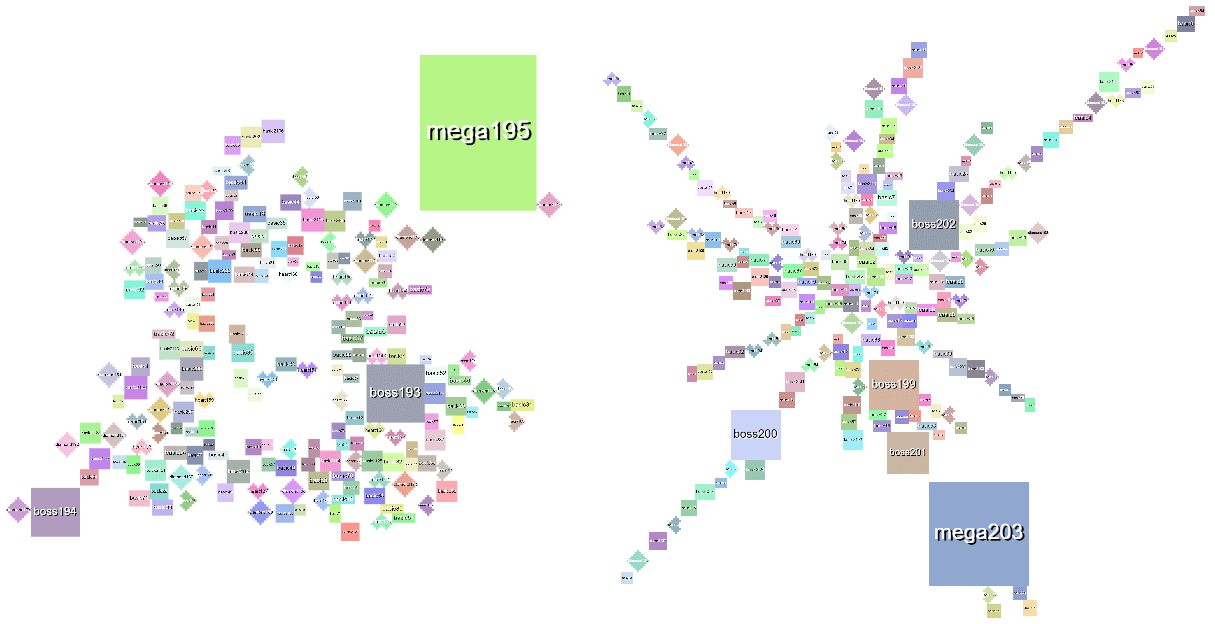
\includegraphics[width=1.0\textwidth]{obrazky/problemy_rozprostreni.png}
    \caption{Vizualizace problémových situací po rozprostření místností. Na obrázku vlevo zanechala místnost \textit{mega195} uprostřed prázdný prostor, který zůstal z~velké části nevyplněn. Na obrázku vpravo je znázorněn problém, kdy posunováním obdélníkových místností pod fixním úhlem dochází k~jejich řazení do paprsků za sebou.}
    \label{img:problemy_rozprostreni}
\end{figure}
Dalším krokem je \textbf{rozprostření místností} po herní úrovni.
Na začátku je iterován seznam místností v~náhodném pořadí.
Pro každou místnost je vybrán náhodný směr od její počáteční pozice (0-359 stupňů).
Následně se procházejí všechny ostatní místnosti a je kontrolováno, zda se s~iterovanou místností neprotínají.
Pokud ano, voláním metody \texttt{getDifferenceInGivenAngle()} je vypočítán vektor, o~který se musí iterovaná místnost přesunout, aby v~kolizi nebyla.
Protože jsou souřadnice celá čísla, úhel vypočítaného vektoru nemusí být exaktně přesný.
Následně je místnost v~daném směru posunuta a kontrola kolizí probíhá od začátku.
\par
Tento systém teoreticky zajišťuje rovnoměrné rozprostření místností po ploše.
Realita je ovšem odlišná.
Prvním problémem jsou příliš velké místnosti.
Pokud se v~konfiguraci nachází obrovská místnost, může dojít k~tomu, že se přesune až jako jedna z~posledních, a tudíž po ní na počáteční pozici zůstane velký nevyplněný prostor (viz obrázek \ref{img:problemy_rozprostreni} vlevo).
Z~tohoto důvodu byl zaveden seznam místností, které jsou již na své finální pozici, a kontrola kolizí probíhá pouze vůči těmto místnostem.
\par
Dalším problémem je, že v~rámci optimalizace rychlosti algoritmu probíhá kontrola kolizí s~tvary doplněnými na obdélník.
Metoda posunování obdélníkových místností pod náhodným, ale stále fixním úhlem pak má tendenci vytvářet \uv{paprsky} místností v~řadě za sebou (viz obrázek \ref{img:problemy_rozprostreni} vpravo).
Tento problém byl vyřešen tak, že se při kontrole kolizí a získávání kolizního vektoru použije náhodná odchylka úhlu v~daném rozsahu.
Díky tomu se může místnost při umísťování náhodně vychýlit ze svého kurzu a tím zaplnit prázdný prostor.
Použitý rozsah pro úhlovou odchylku pak má vliv nejen na výsledný tvar dungeonu, ale také na dobu, za jakou se podaří místnosti rozprostřít bez kolizí (viz graf \ref{img:histogram_uhly}, který je pro lepší znázornění rozdílů prezentován jako histogram dob rozprostírání místností generátorem).
\begin{figure}[ht]
    \centering
    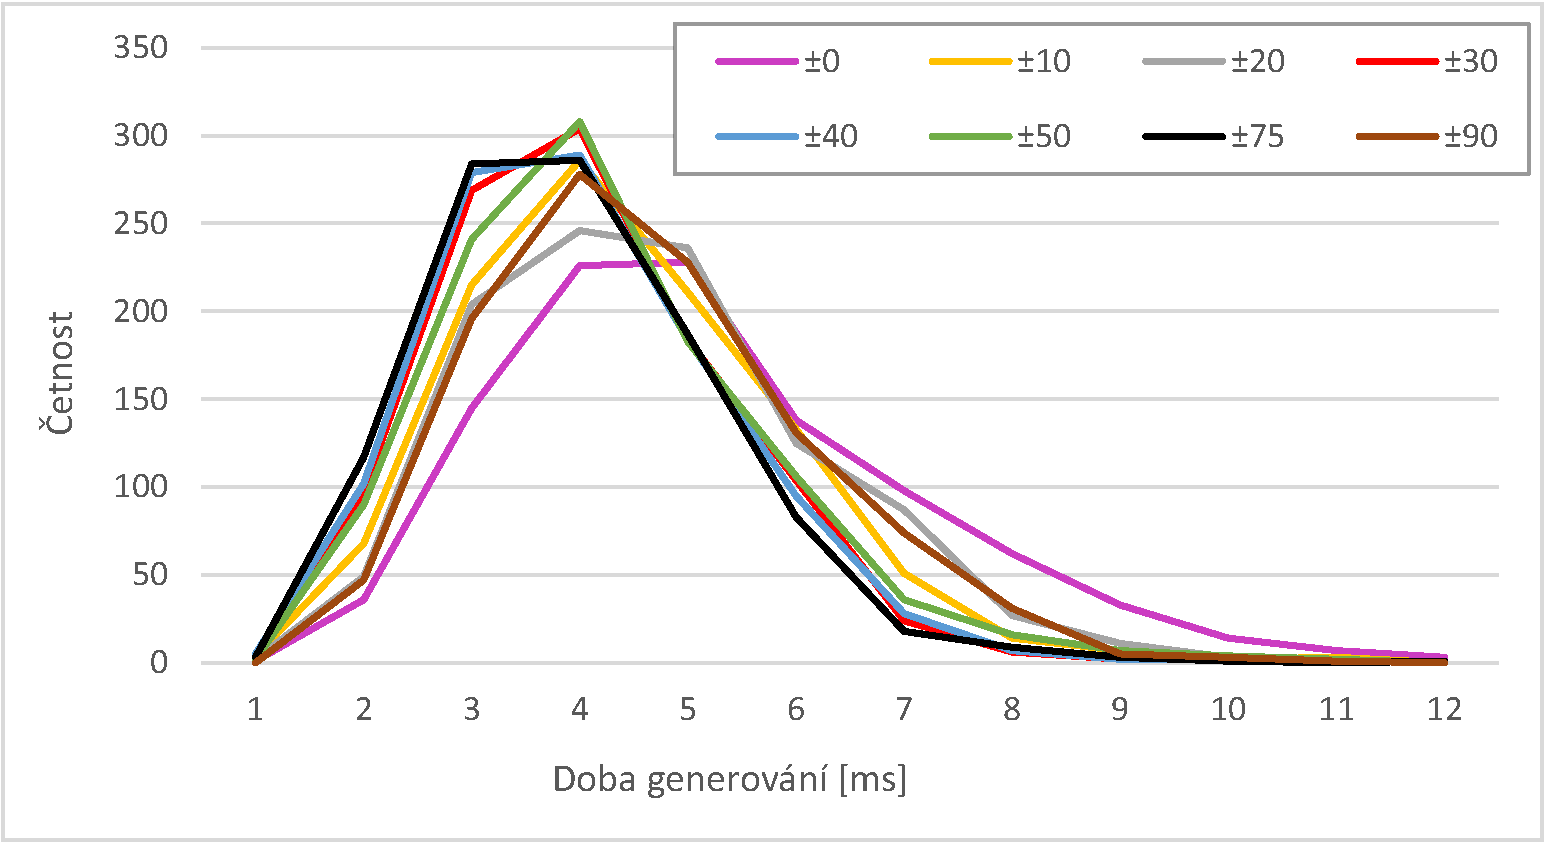
\includegraphics[width=0.75\textwidth]{obrazky/histogram_uhly.pdf}
    \caption{Histogramy dob rozprostírání místností v~závislosti na použité odchylce úhlu. Odchylky uváděné v~legendě jsou ve stupních. Pro každou odchylku z~legendy bylo realizováno 1000 generování s~konfigurací čítající 150 až 300 místností. Měřeno na počítači s~procesorem AMD Ryzen 5 2600, 8 GB RAM, v~prostředí Java 11 s~přidělenými 2 GB RAM a na systému Windows 10.}
    \label{img:histogram_uhly}
\end{figure}
\par
Z~grafu je patrné, že ideální odchylkou pro úhel z~hlediska rychlosti bude $\pm$30, 40 nebo 75 stupňů, přičemž testováním bylo zjištěno, že hodnota 30 stupňů v~malé míře vykazuje tentýž problém s~paprsky a hodnota 75 stupňů už je zase příliš nezajímavá, protože sdružuje všechny místností příliš striktně uprostřed v~kruhu.
Proto byla vybrána úhlová odchylka $\pm$40 stupňů.
\par
Rozprostřené místnosti je dále nutno \textbf{propojit}.
Nejdříve je vytvořena nová instance třídy \texttt{Delaunay\_Triangulation} z~knihovny pro Delaunayovu triangulaci a do jejího konstruktoru jsou předány středy místností jakožto uzly.
Tyto uzly jsou reprezentovány polem instancí \texttt{Point\_dt} pro trojrozměrné body -- třetí rozměr je nevyužit.
Následně je využit iterátor získaný metodou \texttt{trianglesIterator()}, který umožňuje iterovat vytvořenými trojúhelníky (třída \texttt{Triangle\_dt}).
Tyto trojúhelníky jsou poté převedeny na sadu trojic vzájemně propojených místností.
Každá místnost přitom již v~sobě obsahuje informace o~tom, se kterými místnostmi je propojena.
\par
\begin{sloppypar}
Následně je spuštěn algoritmus pro hledání minimální kostry grafu z~knihovny JGraphT.
Nejdříve je vytvořena interní reprezentace grafu, se kterým knihovna pracuje (třída \texttt{SimpleWeightedGraph}).
Ten je naplněn místnostmi dungeonu jakožto body.
Poté jsou přidány hrany mezi body podle toho, jak byly propojeny místnosti v~předchozím kroku.
Hrany jsou následně ohodnoceny podle vzájemné vzdáleností středů místností (bez druhé odmocniny).
Takto připravený graf je předán implementaci algoritmu (třída \texttt{PrimMinimumSpanningTree}) českého matematika Vojtěcha Jarníka (též znám jako Primův algoritmus).
Poté jsou zahozena existující propojení místností, jsou iterovány hrany výsledné struktury a místnosti jsou poté opětovně propojeny.
\end{sloppypar}
\par
V~poslední propojovací fázi jsou s~určitou pravděpodobností (50\,\%) propojovány místnosti, které jsou propojeny pouze s~jednou další místností.
K~tomuto účelu jsou vybrány místnosti, se kterými byla místnost propojena po Delaunayově triangulaci.
Tím jsou do grafu uměle zaneseny smyčky.
K~propojení ovšem dojde pouze tehdy, je-li ohodnocení hrany mezi místnostmi menší nebo rovna průměrnému ohodnocení (aby posléze nedocházelo k~tvorbě příliš dlouhých chodeb).
Protože však ohodnocení nepředstavuje lineární vzdálenost mezi uzly grafu (nebyla využita odmocnina), jako mezní hodnota se používá suma všech ohodnocení vydělená počtem hran vynásobeným třemi.
Tato hodnota byla určena experimentálně a vykazuje dobré výsledky pro malé i velké dungeony.
\par
Poslední důležitou fází generátoru je \textbf{tvorba chodeb}.
Chodby se vytvářejí mezi dvojicemi v~grafu propojených místností.
K~tomu slouží metoda \texttt{createCorridor()}, která má za úkol místnosti propojit chodbou.
Nejdříve je vypočítán přesah hran tvarů místností doplněných na obdélník po ose X a po ose Y.
Pokud přesah existuje, je proveden test toho, zda nejsou místnosti propojeny přirozeně (vzájemnou blízkostí).
Pokud nejsou, jsou stanoveny hrany, mezi kterými se chodba vytvoří.
Chodba se vytvoří ve středu rozsahu, ve kterém mají místnosti přesah.
Před zavoláním metody \texttt{createDirectCorridor()}, která vytváří chodbu mezi dvěma body, jsou tyto body protaženy k~samotným tvarům místností (a nikoliv pouze k~tvarům doplněných na obdélníky).
Pokud místnosti přesah nemají, bude vytvořena chodba ve tvaru písmene L.
Nejdříve je zjištěna vzájemná poloha místností.
Aby se minimalizovalo riziko kolize s~jinou místností nebo chodbou, jsou vybrány nejbližší rohy místností.
Chodba je tak vždy pokud možno co nejkratší.
Následně jsou vytvořeny dvě přímé chodby, které se potkávají ve společném bodě mezi místnostmi (střední vrchol písmene L).
Tyto přímo chodby jsou poté sloučeny v~jednu.
\par
Po vygenerování chodeb je celý dungeon \textbf{normalizován} -- veškeré místnosti i chodby jsou posunuty směrem vpravo dolů do kladných souřadnic.
Bez této úpravy by nebylo možné pracovat s~mřížkou dungeonu reprezentovanou třídou \texttt{Grid}, která podporuje pouze nezáporné souřadnice.
Na konci generátor vrátí strukturu herní úrovně reprezentovanou třídou \texttt{Dungeon}.
Na obrázku \ref{img:dungeon_example} jsou znázorněny různé dungeony, pro jejichž generování byla použita stejná konfigurace.
\begin{figure}[ht]
    \centering
    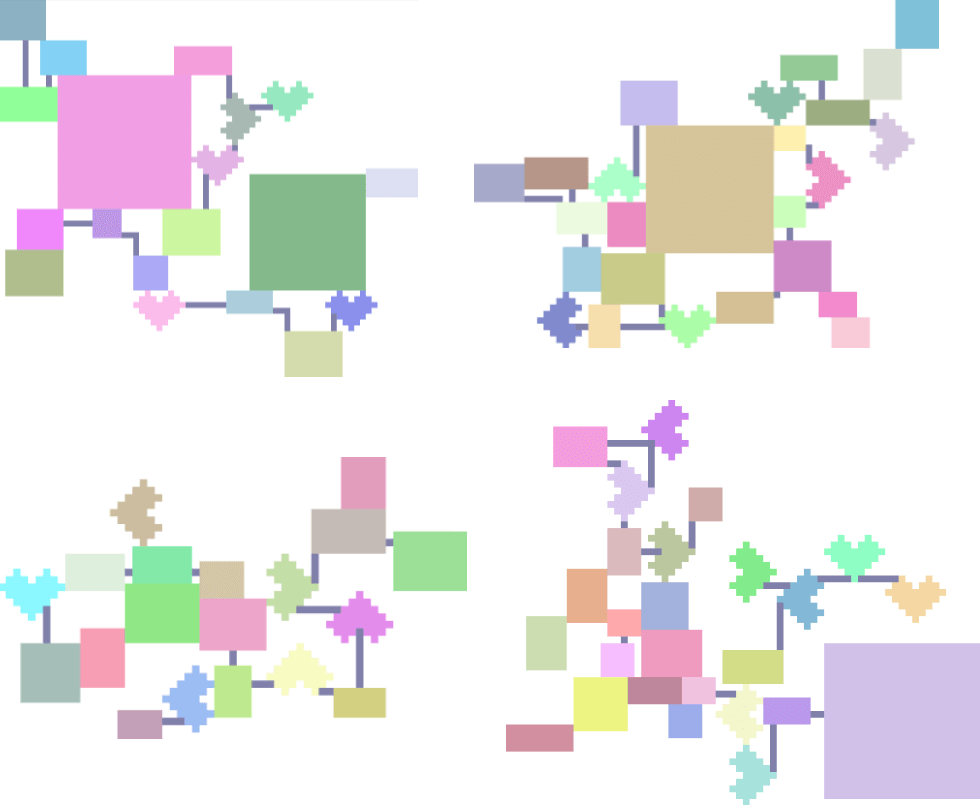
\includegraphics[width=0.75\textwidth]{obrazky/dungeon_example.png}
    \caption{Ukázka dungeonů po dokončení generování. Ve všech případech byla použita totožná konfigurace (největší čtvercová místnost byla označena jako nepovinná). Dungeony vykazují různorodou propojenost i tvary.}
    \label{img:dungeon_example}
\end{figure}

%--------------------------------------------------------------

\chapter{Tvorba vizualizační webové aplikace}
\label{ch:web} % 6

%--------------------------------------------------------------

Souběžně s~vývojem knihovny probíhal také vývoj jednoduché webové aplikace, která dokáže její výstupy vizualizovat.
Některé obrázky publikované v~této práci pochází právě z~této webové aplikace.
Možnost vizualizovat výsledky generované knihovnou její vývoj značně usnadnil, protože vizuální kontrola je lidsky přijatelnější a efektivnější než kontrola výstupu v~textové nebo objektové podobě.
Vývojář si může díky této vizualizaci určit konfiguraci dle libosti a udělat si obrázek o~tom, jak výsledné úrovně vypadají.
Tato kapitola popisuje, jak byla tato jednoduchá webová aplikace navržena, obsahuje souhrn použitých technologií a implementační detaily.

%--------------------------------------------------------------

\section{Analýza požadavků a návrh}
\label{sec:web_navrh}

%--------------------------------------------------------------

Primárním účelem webové aplikace bude \textbf{vizualizace výstupních dat} z~knihovny vytvořené v~předchozích kapitolách.
Webová aplikace proto musí umět zpracovat výstupní data a využít je k~vykreslení místností a chodeb dungeonu.
Místnosti dungeonu však nejsou pouhé čtverce nebo obdélníky -- jsou reprezentovány tvary složenými z~buněk, které musí být přesně vykresleny.
Nad danou místností pak bude uveden název místnosti a její jedinečný číselný identifikátor.
Uživatel by měl být schopen dungeon jednoduše \textbf{procházet} a \textbf{přibližovat či oddalovat}.
Neméně důležitým aspektem je pak \textbf{vykreslení souřadnic} myši, které musí být přepočítány do souřadnic dungeonu.
\par
Webová aplikace bude spouštět generátor a vizualizovat jeho výstup.
Pro spuštění generátoru je potřeba konfigurace, kterou webová aplikace umožní \textbf{zadat přímo} (a vybrat typ souboru ručně) nebo ji \textbf{nahrát ze souboru}.
O~všech chybách musí být uživatel informován.
Uživatel si bude moci určit \textbf{nastavení generátoru}, například které fáze má vykonat nebo zda má vynechat vykreslování některých prvků dungeonu.
\par
Protože se jedná spíše o~webovou pomůcku než o~plnohodnotnou webovou aplikaci, není potřeba implementovat žádný systém přihlašování.
Aplikaci by mělo jít \textbf{snadno spustit} a provádět vizualizace bez zdlouhavých procedur.
\par
Na obrázku \ref{img:web-mockup} je vyobrazen jednoduchý návrh.
Webová aplikace bude velmi jednoduchá -- bude obsahovat úvodní stránku s~nabídkou, dva formuláře (pro souborový a ruční vstup konfigurace), stránku se základními informacemi o~webové stránce a samotnou stránku s~vizualizací.
\begin{figure}[ht]
    \centering
    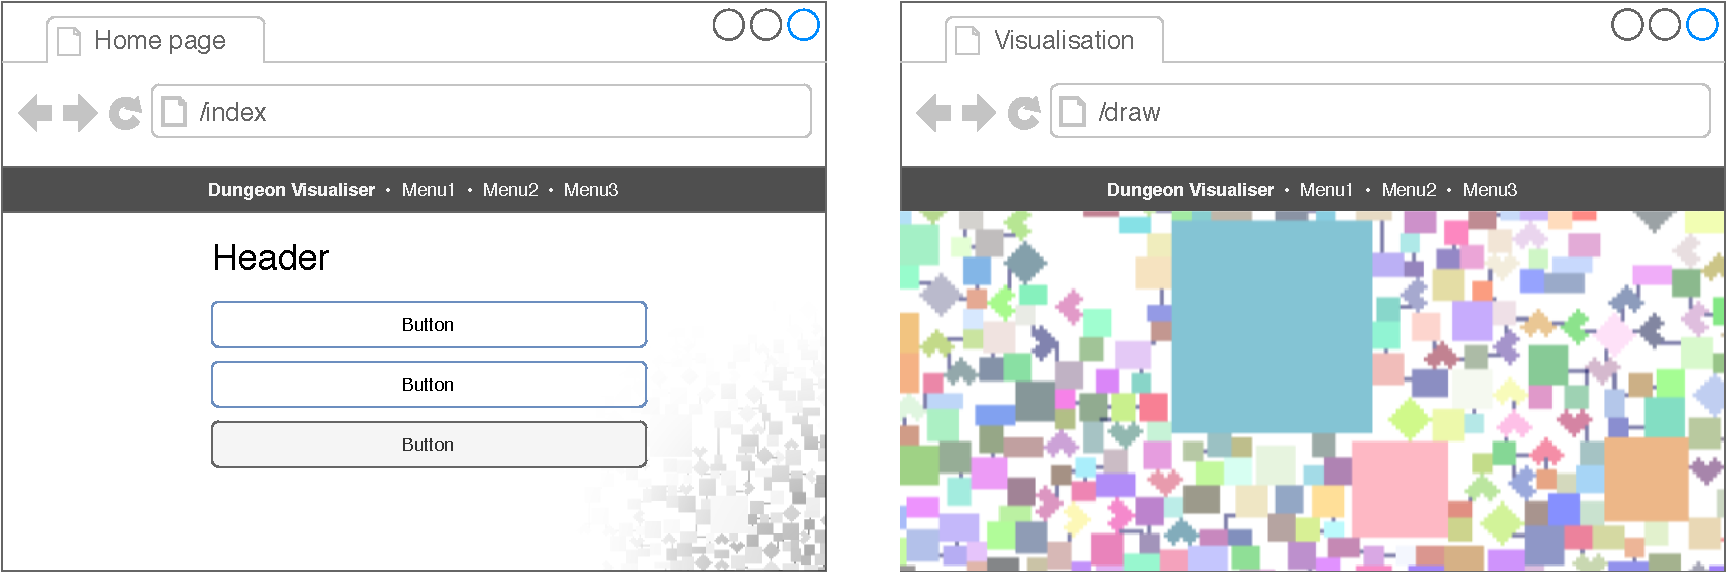
\includegraphics[width=1.00\textwidth]{obrazky/web-mockup.pdf}
    \caption{Návrh webové aplikace pro vizualizaci dungeonů. Vlevo je znázorněno základní rozložení úvodní stránky a vpravo vizualizace dungeonu. Vizualizace bude využívat největší možný dostupný prostor.}
    \label{img:web-mockup}
\end{figure}

%--------------------------------------------------------------

\section{Implementační detaily}

%--------------------------------------------------------------

Pro implementaci byl vybrán jazyk Java a technologie Java EE -- konkrétně aplikační Spring 5\footnote{\url{https://spring.io}} a podprojekt Spring MVC.
Pro prezentační vrstvu byly použity technologie HTML5, CSS3 a sada Bootstrap 4\footnote{\url{https://getbootstrap.com}}.
Pro vývoj šablon byla použita technologie JSP (JavaServer Pages)\footnote{\url{https://www.oracle.com/java/technologies/jspt.html}}, která umožňuje jejich kompilování do servletů.
Tato technologie byla doplněna o~knihovnu dalších standardních značek pro šablony (JSTL -- Standard Tag Library), například cyklus \texttt{foreach}.
Zvažován byl také systém Thymeleaf\footnote{\url{https://www.thymeleaf.org}}, ukázalo se však, že je pro potřeby aplikace nevhodný, protože vykazuje značný pokles výkonu při vpisování dat do šablon s~kódem v~jazyce JavaScript.
Jazyk JavaScript byl totiž základem samotné vizualizace.
Ta je realizována prostřednictvím HTML5 prvku \texttt{Canvas}, na který probíhá vykreslování.
Samotné vykreslování byla provedeno pomocí knihovny PixiJS\footnote{\url{https://www.pixijs.com}}, která veškerou práci usnadňuje a utilizací JavaScriptového API WebGL (Web Graphics Library) pro rendrování na grafické kartě podstatným způsobem zvyšuje výkon.
Pohyb po vizualizaci, její přibližování a oddalování a podporu gest na mobilních zařízeních přidává knihovna Pixi Viewport\footnote{\url{https://github.com/davidfig/pixi-viewport}}.
Veškeré uváděné závislosti byly spravovány systémem Apache Maven\footnote{\url{https://maven.apache.org}}.
Stejným způsobem byla do projektu vložena také vyvinutá knihovna pro procedurální generování dungeonů.
\par
Po otevření úvodní stránky v~prohlížeči a po obdržení HTTP požadavku se aktivuje dispečer \texttt{DispatcherServlet}, který podle URL adresy vyvolá příslušný ovladač (angl. controller), jehož úkolem je požadavek zpracovat a navrátit příslušný pohled (angl. view).
V~případě úvodní stránky bude zavolán \texttt{IndexController}, který vrátí pohled \texttt{index}.
Tento pohled obsahuje pouze tělo samotné stránky (záhlaví a navigační tlačítka v~těle stránky), přičemž záhlaví a zápatí jsou do stránky vloženy ze složky \texttt{views/parts}, která je určena pro dynamicky vkládané části.
Takto složená odpověď je poté zaslána uživateli.
Jakmile uživatel přejde na stránku pro vložení konfigurace, vyplní potřebné údaje a nastavení a data odešle, dojde k~zavolání ovladače \texttt{ManualController}, resp. \texttt{FromFileController} s~modelem naplněným daty.
Po základním ověření (např. případných chybějících údajů) webová aplikace vyvolá metodu \texttt{GenerateDungeonPartially()} a získá výstupní strukturu.
Pokud dojde k~chybě v~konfiguraci nebo generátoru, ovladač vrátí pohled \texttt{error} s~chybovou zprávou a výpisem zásobníku získaným z~výjimky.
Pokud bude generování úspěšné, dojde k~vyvolání pohledu \texttt{draw}, do kterého bude vložen obsah souboru \texttt{visualisation.jsp}.
Tento soubor obsahuje kód v~jazyce JavaScript zodpovědný za vizualizaci.
Do pohledu bude i předán vygenerovaný dungeon, který bude sloužit jako zdroj dat ve vizualizaci.
Uživateli se zobrazí očekávaná stránka a většinu obsahu bude tvořit zmiňovaná vizualizace.

%--------------------------------------------------------------

\section{Výsledná podoba a vyhodnocení}

%--------------------------------------------------------------

Výsledná webová stránka splňuje všechny požadavky uvedené v~části \ref{sec:web_navrh}.
Její podoba je znázorněna na obrázku \ref{img:web-final}.
Webová stránka umožňuje vizualizovat dungeony generované knihovnou a umožňuje uživateli provést konfiguraci před samotnou vizualizací.
Jako možná vylepšení by bylo možné přidat konfiguraci vizualizace bez nutného opětovného generování, ukládání výstupní konfigurace (do textové nebo obrázkové podoby), případně ukládání samotných konfigurací a jejich snadnou úpravu (například možnost určit tvar místností klikáním do matice bodů).
Aplikace umožňuje vizualizaci i na mobilních zařízeních a obsahuje podporu gest, ačkoliv u~větších dungeonů může vizualizace na mobilních zařízeních trvat i desítky sekund.
Aplikace je dodávána v~souboru WAR (Web Application Resource), který umožňuje její velmi snadné zprovoznění na webovém serveru.
Lze ji tak snadno využít k~rychlé a efektivní vizualizaci výstupních struktur knihovny.
\begin{figure}[ht]
    \centering
    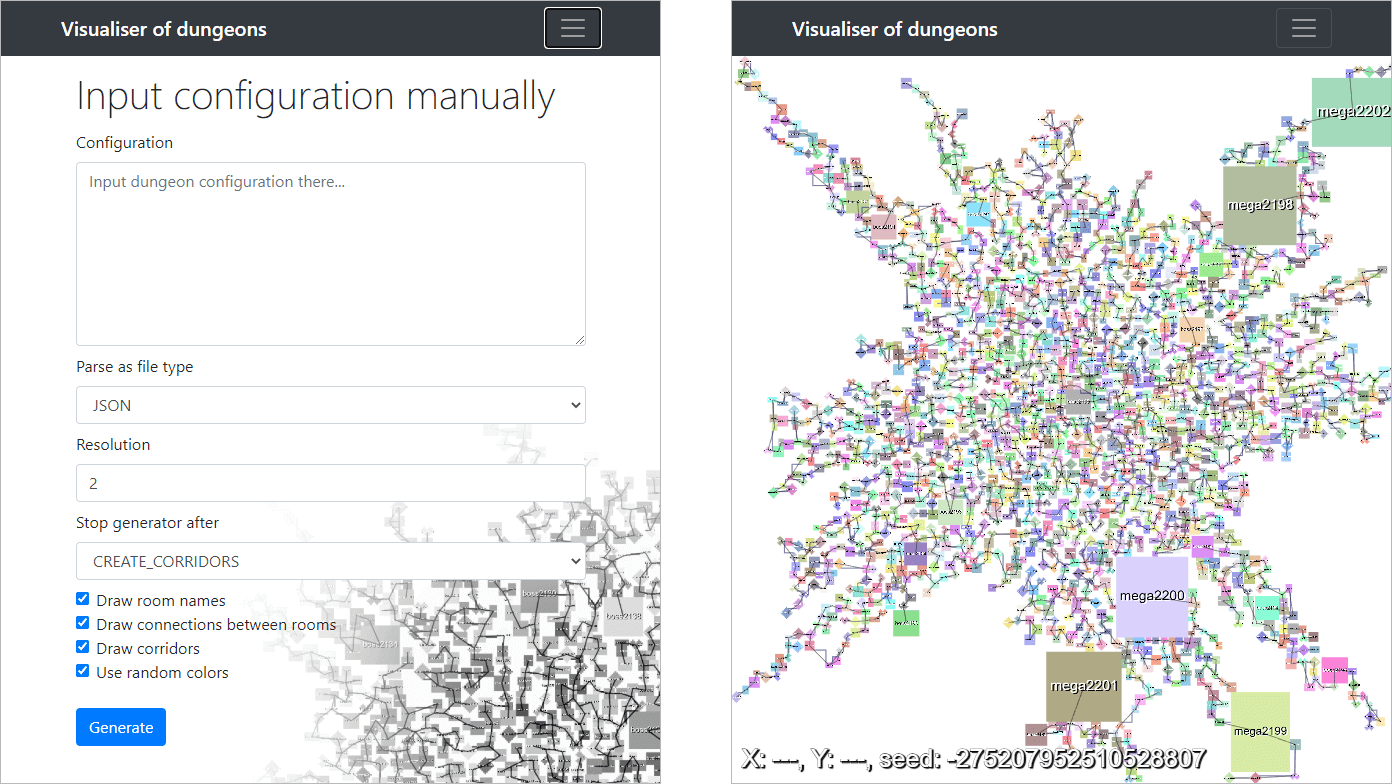
\includegraphics[width=1.00\textwidth]{obrazky/web_final.png}
    \caption{Výsledná podoba webové stránky pro vizualizaci dungeonů. Vlevo je znázorněn formulář pro ruční zadání konfigurace a nastavení generátoru, vpravo je pak samotná vizualizace.}
    \label{img:web-final}
\end{figure}

%--------------------------------------------------------------

% závěr pro kapitolu webové aplikace, grafická podoba

%--------------------------------------------------------------

\chapter{Testování vytvořené knihovny}
\label{ch:testovani} % 7

%--------------------------------------------------------------

Při návrhu knihovny byly v~části \ref{ssec:cilove_vlastnosti} stanoveny cílové vlastnosti, které by měla vytvořená knihovna splňovat.
V~této kapitole bude knihovna posouzena z~hlediska těchto vlastností.
Prověřena bude především praktická využitelnost výstupu generátoru.
Nakonec bude provedeno srovnání s~existujícími řešeními uvedenými v~kapitole \ref{ch:soucasnost}.

%--------------------------------------------------------------

\section{Rychlost generování výstupu}

%--------------------------------------------------------------

Rychlost generování hraje důležitou roli.
Představuje totiž čas, který může hráč potenciálně strávit sledováním načítací obrazovky.
Vývojář si bude s~vysokou pravděpodobností výstup dále upravovat a přidávat další prvky, což bude dobu přípravy herní úrovně ještě více prodlužovat.
Proto je nutné, aby knihovna svou činnost dokončila co nejrychleji.
Veškerá měření rychlosti v~této části probíhala na počítači s~procesorem AMD Ryzen 5 2600, 8 GB RAM, v~prostředí Java 11 s~přidělenými 2 GB RAM a na systému Windows 10.
\par
Při každém měření bylo sledováno trvání jednotlivých fází generátoru zvlášť a celkové trvání.
Bylo provedeno 100 generování dungeonu s~konfigurací čítající přesně 500 místností.
Každé generování bylo provedeno s~náhodným semínkem a výsledky (průměrné doby trvání) jsou znázorněny v~grafu \ref{img:graph_speed}.
Navzdory vysokému počtu místností (500 místností uživatel pravděpodobně nebude nikdy potřebovat, typické dungeony obvykle obsahují maximálně desítky místností) trvalo generování průměrně desetinu sekundy.
\begin{figure}[ht]
    \centering
    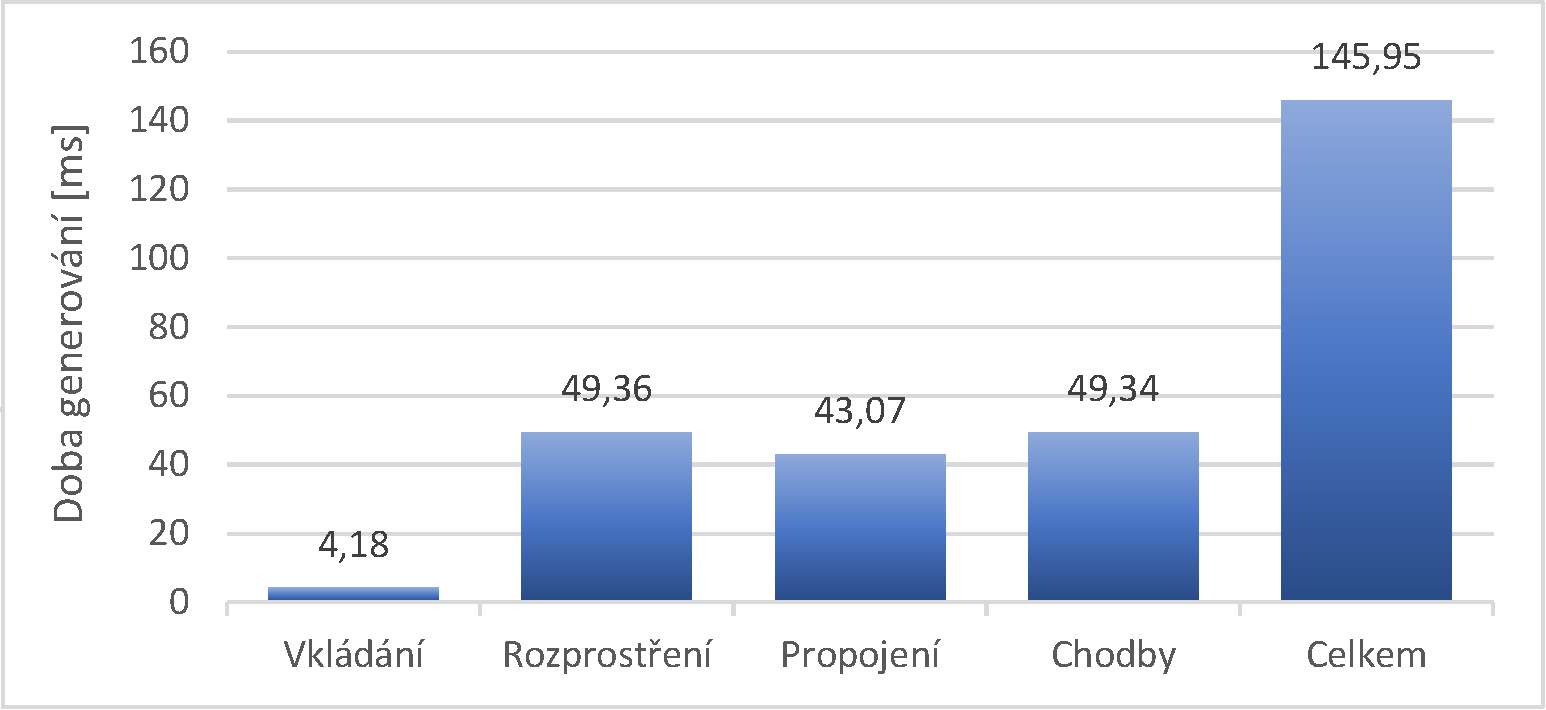
\includegraphics[width=0.75\textwidth]{obrazky/graph_speed.pdf}
    \caption{Rychlost generování dungeonů během jednotlivých fází a celkem. Jedná se průměrné doby při generování 100 dungeonů s~konfigurací čítající přesně 500 místností.}
    \label{img:graph_speed}
\end{figure}
\par
Dále bylo analyzováno celkové trvání generování v~závislosti na počtu místností.
Opět bylo vždy vygenerováno 100 dungeonů a počty místností byly navyšovány po stovkách.
Průměrné doby trvání jsou uvedeny v~grafu \ref{img:graph_speed2}.
Z~grafu je patrné, že se doba trvání spolu s~počtem místností zvyšuje exponenciálně a nikoliv lineárně.
To je očekávané chování, protože například při rozprostírání místností se musí při přemísťování každé místnosti kontrolovat kolize se všemi ostatními.
\begin{figure}[ht]
    \centering
    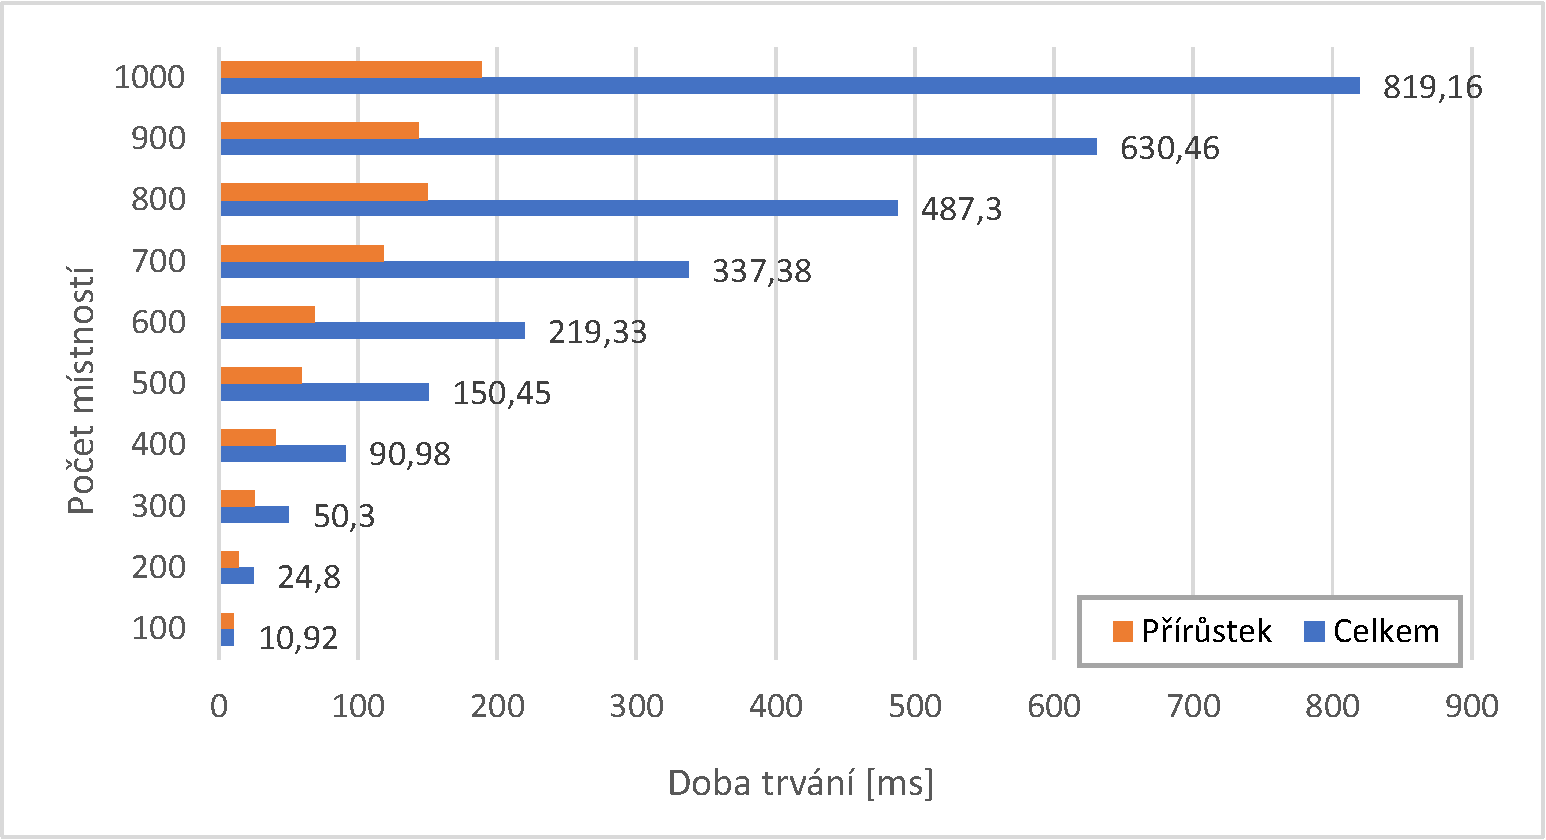
\includegraphics[width=0.75\textwidth]{obrazky/graph_speed2.pdf}
    \caption{Rychlost generování dungeonů v~závislosti na počtu místností. Jedná se průměrné doby při generování 100 dungeonů.}
    \label{img:graph_speed2}
\end{figure}

%--------------------------------------------------------------

\section{Parametry a přizpůsobitelnost výstupu}

%--------------------------------------------------------------

Knihovna umožňuje definovat počet a tvar místností, které jsou poté rozmístěny náhodně a náhodně propojeny chodbami.
Z~tohoto důvodu je knihovna vhodná spíše pro generování strukturovaných dungeonů, a nikoliv pro generování úrovní s~menší mírou uspořádanosti (například jeskyní).
\par
Výstupní struktura knihovny je fixně určena, nabízí však uživateli možnost doplnit vygenerované místnosti a chodby o~prvky podle libosti (například nepřátele nebo poklady pro hráče).
Uživatel má k~dispozici výsledné tvary místností i chodeb v~přehledné maticové struktuře.

%--------------------------------------------------------------

\section{Intuitivnost a jednoduchost použití}

%--------------------------------------------------------------

Pro vygenerování dungeonu je potřeba spustit jedinou metodu a předat jí konfiguraci.
Uživatel si může vybrat, zda použije nabízené rozhraní API nebo zadá konfiguraci v~souboru.
Další možností je přímé spuštění knihovny a zadání vstupní souborové konfigurace, kdy knihovna vygeneruje výstupní soubor, případně soubor s~chybovou zprávou.
Uživatel nejdříve určí tvary místností a ty přiřadí místnostem.
Pro zjednodušení má uživatel k~dispozici šablony generující náhodné tvary.
Tvary však může vytvářet i ručně jednoduchým zapsáním matice znaků.
Další ukázkou jednoduchosti použití může být výpis \ref{code:spigotplugin}, kde je demonstrováno generování dungeonu v~počítačové hře pomocí několika málo řádků kódu.
Výstupní struktura pak obsahuje samotné místnosti a chodby.
Uživatel získá informace o~jejich pozici, tvaru a vzájemného propojení.
Dalším možným způsobem, jak přistupovat k~výstupním datům, je mřížka buněk dungeonu, přičemž každá buňka obsahuje pozici, typ a případně i odkaz na příslušnou místnost či chodbu, kterou reprezentuje.
\par
Knihovna je doplněna o~JavaDoc komentáře, které umožňují vygenerování textové dokumentace pro koncové uživatele.
Díky tomu má uživatel přehled nad tím, jak knihovnu používat.
Co se týče případných chyb, uživatel je informován o~chybách v~konfiguraci, chybách v~generátoru, případně ostatních výjimkách (např. vstupně-výstupní chyby při práci se soubory) a měl by tak být schopen chybu opravit.

%--------------------------------------------------------------

\section{Praktická využitelnost}

%--------------------------------------------------------------

Funkčnost knihovny byla ověřena i prakticky přímo v~počítačové hře.
K~tomuto účelu byla vybrána hra \textit{Minecraft}, která umožňuje přetvářet herní svět ze stavebních bloků, což z~ní činí dobrou volbu, vzhledem k~povaze výstupní struktury knihovny, která je složena z~diskrétních částí (buněk).
Knihovna byla do hry implementována jako plugin serverového API Spigot MC\footnote{\url{https://www.spigotmc.org}}.
Spigot MC funguje jako prostředník mezi serverovou částí jádra hry Minecraft a vývojáři a umožňuje jim prostřednictvím pluginů modifikovat jeho funkčnost.
Plugin napsaný pro tuto práci funguje následovně:
\begin{enumerate}
    \item Vytvoř instanci třídy \texttt{WorldCreator} a nastav jej tak, aby vytvářel ploché světy.
    \item Pomocí třídy \texttt{Bukkit} a statické metody \texttt{createWorld()} vytvoř nový svět (pokud již existuje, pouze se načte a tím činnost pluginu končí).
    \item Pokud svět předtím neexistoval, vytvoř jednoduchou konfiguraci dungeonu a ten vygeneruj.
    \item Projdi mřížku ve výstupní struktuře a případné místností a chodby umísti do nově vygenerovaného světa.
\end{enumerate}
Tímto jednoduchým způsobem je možné vytvořit funkční dungeon přímo ve hře (viz výpis kódu \ref{code:spigotplugin}).
\lstinputlisting[style=Java,language=Java,caption={Ukázka praktického použití knihovny ve hře Minecraft. Nejdříve je jednoduše vygenerován dungeon a ten je poté za pomoci mřížky vložen do herní úrovně.},label={code:spigotplugin}]{kody/spigotplugin.java}
Výsledek je znázorněn na obrázku \ref{img:mc-dungeon}.
Demonstrace je velmi jednoduchá a slouží pro účely této práce.
Aby bylo možné dungeon projít, bylo by nutné algoritmus pluginu dále upravit, aby vytvářel \uv{duté} místnosti a aby byly chodby širší.
K~tomuto účelu stačí upravit měřítko algoritmu, aby pro jednu buňku mřížky ve výstupní struktuře vytvořil nikoliv jeden blok, ale 2x2 nebo více bloků, čímž vznikne prostor pro další manipulaci.
\begin{figure}[ht]
    \centering
    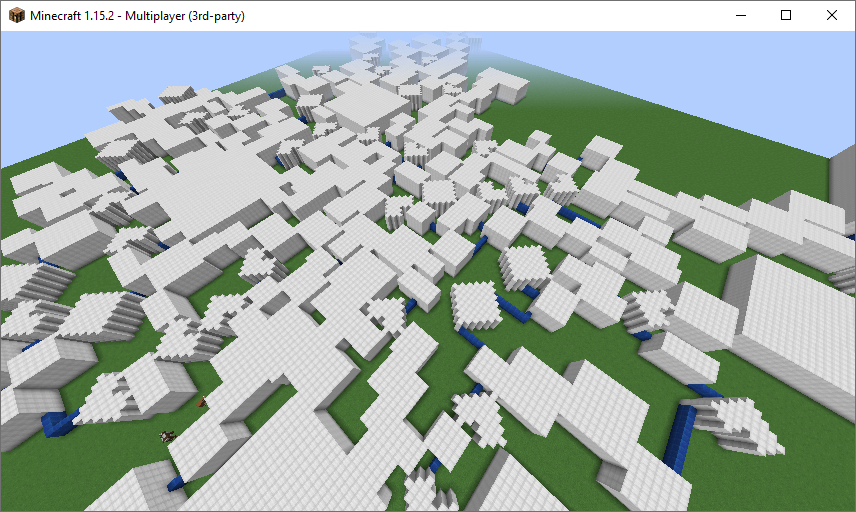
\includegraphics[width=0.80\textwidth]{obrazky/mc-dungeon.png}
    \caption{Náhodný dungeon vygenerovaný pomocí vytvořené knihovny ve hře \textit{Minecraft}.}
    \label{img:mc-dungeon}
\end{figure}

%--------------------------------------------------------------

\section{Spolehlivost generátoru}

%--------------------------------------------------------------

Výstup generátoru vždy odpovídá zadané vstupní konfiguraci.
Uživatel může nepovinné místnosti označit tak, že při zadávání jejich počtu připustí nulový počet.
Generátor zajišťuje, že celý dungeon bude možné projít a že žádná místnost nezůstane nepropojena.
\par
Při testování bylo odhaleno, že u~velmi velikých dungeonů občas dochází k~protnutí chodby a cizí místnosti.
Tuto chybu lze opravit implementací složitějšího algoritmu pro hledání cesty chodby, což však pravděpodobně bude mít negativní dopad na celkovou rychlost generátoru.
Dalším zjištěným problémem je, že větší místnosti mají tendenci být \uv{vytlačeny} k~okrajům místnostmi menšími.
Tento problém se dá z~části vyřešit tím, že se před rozprostřením místností stanoví takové pořadí místností, ve kterém budou místnosti zaujímající větší plochu upřednostněny před menšími.

%--------------------------------------------------------------

\section{Různorodost výsledných struktur}

%--------------------------------------------------------------

Základem knihovny je procedurální generování.
Ačkoliv se v~tomto případě jedná o~pouhé generování místností a chodeb, i přesto může mít velký vliv na celkovou kompozici herní úrovně a její vnímání hráčem.
Na repetitivnost a stereotyp mají v~tomto případě vliv tři zásadní faktory:
\begin{enumerate}
    \item Konfigurace vytvořené vývojářem a předané knihovně.
    \item Schopnost knihovny generovat různorodé herní úrovně.
    \item Obsah herních úrovní a ostatní aspekty hry, například příběhová linie.
\end{enumerate}
Z~pohledu této práce se první a poslední bod nedají nijak zvlášť ovlivnit a jsou v~rukou vývojáře.
Druhý bod tato knihovna splňuje pouze do té míry, že v~případě použití náhodného semínka má vývojář jistotu, že bude rozložení herní úrovně vždy jedinečné.
Jediným výraznějším prvkem různorodosti v~konfiguraci jsou \textbf{číselné rozsahy} u~parametrů šablon a u~počtu místností.
Co se týče rozložení místností, použitý algoritmus podle očekávání soustřeďuje většinu místností do středu.
Vytvořením jednoduché teplotní mapy pozic buněk dungeonu (obrázek \ref{img:heatmap}) lze však vysledovat, že u~okrajů se místnosti sdružují spíše v~rozích, a nikoliv rovnoměrně.
Po bližším přezkoumání lze v~teplotní mapě vypozorovat jev, kdy se větší místnosti častěji nacházejí u~okrajů herní úrovně.
Použitá metoda rozložení místností tak vykazuje určité nedostatky, které se projevují v~určitých mezních situacích (velmi velké množství generovaných místností nebo definice místností, které svou plochou výrazně přesahují plochy ostatních místností).
\begin{figure}[ht]
    \centering
    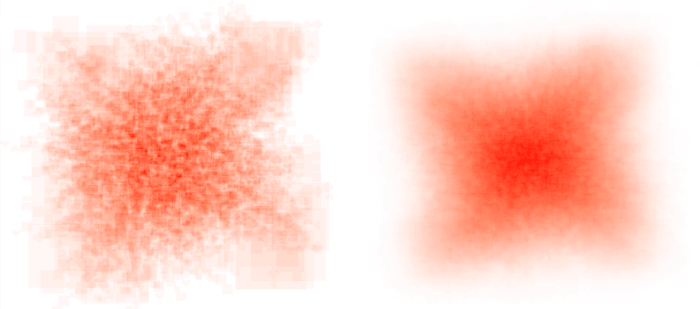
\includegraphics[width=0.80\textwidth]{obrazky/heatmap.png}
    \caption{Teplotní mapa reprezentující četnost místností na určitých místech dungeonu. Červenější odstín značí větší četnost. Na obrázku vlevo bylo vygenerováno 30 dungeonů, na obrázku vpravo 750 dungeonů. Konfigurace obsahovala okolo 250 místností.}
    \label{img:heatmap}
\end{figure}

%--------------------------------------------------------------

\section{Opakovatelnost výstupu}

%--------------------------------------------------------------

Celá knihovna byla navržena tak, aby umožňovala zadání semínka generátoru, podle kterého generátor pracuje.
Byly použity Java kolekce s~konstantním pořadím iterování (například \texttt{LinkedHashSet}, což je množina, která interně využívá dvoucestného spojového seznamu a zachovává tak pořadí prvků podle toho, jak byly vloženy) a globálně sdílený generátor náhodných čísel.
\par
Semínko lze zadat do konfigurace prostřednictvím souboru nebo přímo v~rozhraní API.
Knihovna garantuje, že pokud bude pro generování opakovaně zadána kombinace totožných parametrů a semínka, výstup bude vždy stejný.
Tento jev byl také otestován a nepodařilo se najít žádnou konfiguraci, ve které by neplatil.

%--------------------------------------------------------------

\section{Srovnání knihovny s~existujícími řešeními}

%--------------------------------------------------------------

V~kapitole \ref{ch:soucasnost} byly představeny knihovny a hry, které souvisí s~problematikou procedurálního generování dungeonů.
V~této části bude knihovna ve stručnosti s~těmito řešeními porovnána.
\par
Herní úrovně v~představené hře Rogue z~roku 1980 se skládaly z~9 obdélníkových místností s~náhodnými rozměry a tyto místnosti byly propojeny chodbami.
Vytvořená knihovna dokáže díky tvarovým šablonám generovat náhodné čtvercové i obdélníkové místnosti, přičemž uživatel může určit jejich počet.
Nemůže však nijak ovlivnit jejich pozici, která je určena náhodně.
Generování takto malých dungeonů je však velmi rychlé a proto není problém vygenerovat například 100 dungeonů a vybrat si z~nich ten nejvhodnější.
Díky metodám poskytovaným knihovnou může vývojář velmi rychle určit vzájemnou polohu místností.
\par
Generátor herních úrovní ve hře Diablo 1 z~roku 1996 je typickou ukázkou generátoru, jimž vytvářené úrovně jsou příliš specifické, než aby se daly pokrýt univerzálně použitelnou knihovnou.
V~počátečních herních prostředích by však bylo možné úrovně vygenerované touto knihovnou použít jako základ a dále s~nimi pracovat, například postupným rozšiřováním o~přiléhající místnosti a rozšířené chodby a další požadované detaily.
Vytvořenou knihovnu by však nebylo možné použít na generování jeskyní, protože je její výstup příliš uspořádaný -- to však ani nebylo cílem, jeskyně jako taková nesplňuje charakteristiku dungeonu.
\par
Světy vytvářené ve hře Don't Starve jsou sekvenčně řazené podle úloh a tudíž je vytvořená knihovna nedokáže nijak napodobit.
Vývojář ovšem může implementovat generátor vlastních tvarů pro místnosti v~textové podobě a vytvořit v~konfiguraci místnosti, kterým tvary přiřadí.
Generátor je poté schopen tyto místnosti vhodným způsobem vložit a propojit a vývojář může některé z~nich použít a přiřadit jim účel, vlastnosti a vizuální prvky až posléze.
\par
V~části \ref{ssec:dungeongenerator_jongallant} byl představen generátor \textit{DungeonGenerator}, kterým byly inspirovány některé fáze generátoru použitého v~této knihovně.
Tento generátor pro systém Unity nabízí pouze velmi omezenou sadu vstupních parametrů, které jsou navíc pevně zapsány v~knihovně.
Nenabízí žádné rozhraní ani možnost použít knihovnu mimo systém Unity, protože je závislý na fyzikálním systému Unity a využívá jeho algoritmus pro rozprostírání místností.
Uživatel nemá navíc žádnou kontrolu nad tím, jaké místnosti generátor vygeneruje a vytvářené chodby mezi místnostmi jsou doplňovány jako izolované buňky bez reference na místnosti, které chodba propojuje.
Knihovna vytvořená v~této práci veškeré tyto problémy řeší a nabízí i další funkce, například možnost semínka, určování tvarů a počtů místností, plnou souborovou podporu, možnost spouštění jako program a plně dokumentované rozhraní.
Obě knihovny na výstupu uživateli poskytují jak grafovou reprezentaci místností, tak dvourozměrnou mřížku.
\par
Knihovna \textit{Rot Web API} představená v~části \ref{ssec:rotwebapi} je značně omezená co se parametrů a výstupu týče, ukazuje však velmi zajímavý koncept generátoru jakožto webové služby, díky čemuž lze tuto knihovnu používat z~kteréhokoliv systému nezávisle na programovacím jazyku.
Pro použití je však nutné knihovnu zprovoznit jako webový server.
Knihovna odpovídá ve formátu JSON, který je široce používán například v~architektuře REST.
Knihovna vytvořená v~této práci podporuje jak formát JSON, tak formáty YAML a XML a umožňuje používání nezávisle na jazyku díky tomu, že je spustitelná jako program a umožňuje souborovou komunikaci.
Výhodou je, že ji uživatel nemusí složitě nastavovat a nepotřebuje webový server.
Nevýhodou je nutnost mít na cílovém počítači nainstalováno běhové prostředí Javy.

%--------------------------------------------------------------

\chapter{Zhodnocení výsledků práce a závěr}
\label{ch:zaver} % 8

%--------------------------------------------------------------

Cílem této práce bylo analyzovat existující metody procedurálního generování, zejména metody pro generování herních úrovní typu dungeon, navrhnout a implementovat prakticky použitelnou knihovnu umožňující zadání konfigurace a vygenerování herní úrovně a následně vytvořit webovou aplikaci, ve které bude knihovna prakticky využita a zároveň bude vizualizací demonstrovat i funkčnost knihovny.
\par
Vytvořená knihovna generuje strukturované místnosti propojené chodbami a je připravena pro použití ve hrách.
Hlavními přednostmi je rychlost generování, jednoduchost použití a dobrá konfigurovatelnost.
Nevýhodou je omezená použitelnost v~případě, že má vývojář specifičtější požadavky na uspořádání dungeonů.
Knihovna umožňuje zadání konfigurace prostřednictvím poskytnutého rozhraní, případně načtením ze souboru, a vygenerovaný dungeon lze rovněž uložit do souboru.
Knihovna je využitelná i jako spustitelný program, což umožňuje její použití nezávisle na programovacím jazyku.
Navržená webová aplikace umožňuje tyto dungeony jednoduchým způsobem vizualizovat a usnadňuje tak testování konfigurací a výstupů.
Funkčnost knihovny byla dále prověřena testováním a jejím použitím v~počítačové hře.
\par
Během vytváření knihovny bylo potřeba zvážit uživatelské požadavky a aplikovat techniky, které je dokážou uspokojit.
Knihovna generuje místnosti, ty zařazuje do kontextu grafů a prostřednictvím Delaunayovy triangulace a hledání minimální kostry s~grafem dále pracuje.
Nezanedbatelnou výzvou byl i výběr vhodné techniky pro rozprostření místností na rovině, kde se ukázalo, že drobné změny mohou mít velký vliv na výsledek.
\par
Při práci na knihovně a webové aplikaci jsem si procvičil práci s~literaturou i internetovými zdroji, osvojil jsem si princip fungování různých technik procedurálního generování a musel jsem se zamyslet nad tvorbou knihovny z~hlediska její použitelnosti, vytvořit důkladný návrh a ten realizovat.
\par
Knihovna nabízí spoustu prostoru k~vylepšování a rozšiřování.
Systém generování tvarů na základě šablon se ukázal jako velmi užitečný, proto by bylo jistě vhodné, aby knihovna umožňovala naprogramovat šablony vlastní.
Knihovna obsahuje jeden generátor, který pracuje v~několika fázích.
Tyto fáze by bylo vhodné proměnit na univerzálně použitelné a zvláště konfigurovatelné komponenty, které by se daly použít ve vlastních generátorech.
S~tím by byla spojena možnost upravovat strukturu vstupní konfigurace a výstupních dat.
Zajímavou možností by byla implementace generátoru, který by umožnil tvorbu místností v~určitém sledu.
Například místnost s~nepřítelem, za kterou by vždy následovala místnost s~pokladem.
K~tomu by byl ovšem potřeba dodatečný výzkum.